\documentclass[12pt]{report}

% Set input file encoding to UTF-8
\usepackage[utf8]{inputenc}

% Use Stanford Thesis Package
\usepackage{suthesis-2e}

% Additional packages
\usepackage{amssymb,amsmath,amsfonts,mathtools}
\usepackage{xcolor}
\usepackage{hyperref}
\usepackage{bm}
\usepackage{subcaption}
\usepackage{graphicx}
\usepackage{graphbox}
\usepackage{multirow}
\usepackage{braket}
\usepackage{minted}
\usepackage{mdframed}
\surroundwithmdframed{minted}
\usepackage{pgfplots}
\pgfplotsset{compat=1.18}
\usepackage[numbers,sort&compress]{natbib}
\bibliographystyle{abbrvnat}

\captionsetup{size=small}
\captionsetup[sub]{size=small}

% Number subsubsections to enable referencing them
\setcounter{secnumdepth}{3}

% Set up link and citation colors
\hypersetup{
    colorlinks,
    linkcolor={blue!80!black},
    citecolor={blue!80!black},
    urlcolor={blue!80!black}
}

% Set up custom autoref link text
\def\chapterautorefname{Chapter}
\def\sectionautorefname{Section}
\def\subsectionautorefname{Subsection}
\def\subsubsectionautorefname{Subsubsection}
\def\itemautorefname{}

% Additional math commands
\newcommand{\tensorOne}[1]{\bm{#1}}
\newcommand{\tensorTwo}[1]{\bm{#1}}
\newcommand{\tensorFour}[1]{\mathbb{#1}}
\newcommand{\linearOperator}[1]{\mathcal{#1}}

\renewcommand{\vec}[1]{\tensorOne{#1}}
\newcommand{\mat}[1]{#1}

\renewcommand{\P}{\linearOperator{P}}
\newcommand{\R}{\linearOperator{R}}
\newcommand{\M}{\linearOperator{M}}

% New math operators to be typeset in normal text
\DeclareMathOperator{\Diag}{diag}
\DeclareMathOperator{\Rowsum}{rowsum}
\DeclareMathOperator{\Trace}{tr}
\DeclareMathOperator{\Nnz}{nnz}

\newcommand{\Colorcircle}[1]{\protect\tikz\protect\draw[black,fill=#1] (0,0) circle (.5ex);}
\newcommand{\Colorsquare}[1]{\protect\tikz\protect\draw[black,fill=#1] (0,0) rectangle (1ex,1ex);}

% Basic thesis information
\dept{Energy Resources Engineering}
\title{Multiscale Solver for Subsurface Poromechanical Problems}
\author{Sergey Klevtsov}
\principaladviser{Hamdi Tchelepi}
\firstreader{Louis Durlofsky}
\secondreader{Nicola Castelletto}

% Enable lists of tables/figures
\tablespagetrue
\figurespagetrue

\begin{document}
 
\beforepreface

\prefacesection{Abstract}


\prefacesection{Acknowledgments}


\afterpreface

\chapter{Introduction}
\label{ch:introduction}

% ===================== SECTION =====================
\section{Motivation}

Understanding, quantifying and predicting the behavior of subsurface poromechanical systems is of critical importance in many applications in the energy industry and beyond, from geological storage of CO\textsubscript{2}, to oil and gas production, to geothermal reservoirs, to management of groundwater resources.   In many of these applications, fast and accurate predictions are necessary to optimize the cost of operation, assess uncertainties and manage risks associated with complex interactions between various physical phenomena, including land subsidence, induced seismicity, fault reactivation, seal and wellbore integrity.   With the increasing cost and complexity of these projects, simple analytical models no longer provide the necessary level of detail, and numerical modeling has become an indispensable tool aiding researchers, engineers and regulatory agencies alike.

Subsurface numerical models are constantly growing in their size and complexity, placing an ever increasing demand for robust and scalable computational methods and tools.   Typical reservoir models are characterized by large spatial (tens of kilometers) and temporal (tens to hundreds of years) extents as well as heterogeneous and anisotropic petrophysical properties (such as porosity, permeability and mechanical moduli) possessing multi-scale correlation structures that require high-fidelity geological models in order to resolve the important fine-scale details.   Consequently, a simulation tool must be able to perform thousands of time steps with tens of millions of unknowns to solve for at every step in a reasonable amount of time.   Many of these highly-detailed models have abandoned the computationally attractive framework of logically structured Cartesian grids and are described using partially or fully unstructured meshes, owing to their ability to accurately represent important geological and stratigraphic features such as faults and pinch-outs.   Some of the solution approaches previously developed may not be applicable to these complex meshes, requiring more flexible techniques to be sought.

In addition, the complex nature of physical phenomena involved requires solving multiple governing equations that are often tightly coupled, leading to systems with degrees-of-freedom of mixed nature, that often require specialized algorithms and solution schemes to deal with.   In recent years, simulations involving coupled geomechanics, porous media flow, heat transfer, multiphase multi-component transport and chemical reactions have begun to emerge.   Moreover, with a large amount of uncertainty that is inherently present in subsurface models due to limited observations available, statistically generated ensembles consisting of thousands of realizations and dozens of modeling scenarios must be simulated to allow for data-driven decision making.   All of these requirements present a formidable challenge to existing and upcoming modeling tools. 

A large number of techniques have been developed to reduce the size of models and make them more feasible for both forward and inverse modeling, including upscaling as well surrogate and reduced-order models.   Most recently, advancements in supervised machine learning made it possible to train large-scale neural network models to predict behavior of subsurface systems by generalizing observations and extracting patterns from simulation results.   We note that whether or not these models are ultimately successful as prediction tools, they still need large volumes of training data that must be generated by physics-driven simulation.   As such, the demand for fast and accurate forward modeling software continues to increase.

At the same time, improvements in design and manufacturing of processing units have approached the physical limits of a single chip, and all modern computing hardware is increasingly parallel at every level, from multi-core CPUs to GPU (graphical processing units) accelerators featuring thousands of cores, to wafer-scale systems, to computing clusters with hundreds of nodes.   In order to keep up with the computational requirements, existing techniques must be continuously improved and new scalable algorithms must be developed that are capable of taking advantage of parallel hardware efficiently.   In the area of subsurface modeling, multi-level and multi-scale methods have been shown to be particularly attractive as robust and high-performing solvers and preconditioners.

% ===================== SECTION =====================
\section{Problem Statement}

\subsection{Governing Equations and Discrete Problem}

\subsection{Solution Approaches for Two-way Coupled Systems}

\subsection{Iterative Solvers and Preconditioning}

% ===================== SECTION =====================
\section{Dissertation Outline}

\chapter{Multilevel Multiscale Solver for Poromechanics}
\chaptermark{Multiscale Solver for Poromechanics}
\label{ch:multiscale_poromechanics}

This chapter details the main contribution of present work --- the development of an efficient multi-level multiscale preconditioned Krylov solver tackling fluid flow and mechanical deformation in porous media. The chapter is organized as follows. \autoref{sec:related_work} presents the necessary background and related work in the area of multilevel solvers that our development builds upon. The adaptation of one of the previously developed multiscale techniques --- the Multiscale Restricted Smoothing Basis (MsRSB) method --- to the problems of interest is motivated and explained in \autoref{sec:enhanced_msrsb}.   \autoref{sec:msrsb_coarsening} deals with the complexity of constructing agglomeration-based unstructured coarse grids.   Then, in \autoref{sec:msrsb_interpolation}, procedures for the iterative construction of two types of basis functions (nodal and cell-centered) are detailed.   \autoref{sec:coupled_precond} completes development of the full preconditioner by describing our approaches to combining interpolation operators and smoothers, as well as handling of wells and transport unknowns.   Properties of the scheme are investigated in \autoref{sec:msrsb_examples} using a set of numerical examples designed to test the algorithmic scalability and robustness of the method.   Finally, the chapter concludes with a summary in \autoref{sec:msrsb_summary}.

% ===================== SECTION =====================
\section{Related Work}
\label{sec:related_work}

Various multilevel methods for accelerating solution of linear systems have been developed over the span of over 50 years, but they have received particular interest in the area of subsurface modeling in the past two decades.    The most prominent types of multilevel approaches are \textit{mutligrid} (geometric and algebraic) and \textit{multiscale} methods, which bear a lot of similarities despite being formulated on different principles.    This section briefly reviews the history, background and recent advancements relevant to the development of the multiscale method in present work.

\subsection{Multigrid Methods}
\label{subsec:related_work_multigrid}

Multigrid was first introduced in \cite{Fedorenko1962} and analyzed and extended in \cite{Fedorenko1964,Bakhvalov1966,Nicolaides1975,Brandt1977} as a way of accelerating a relaxation procedure (such as Gauss-Seidel) for a finite-difference discretization of homogeneous Poisson's equation on a structured 2D grid.   Today it is one of the most efficient methods for solving a wide class of linear systems stemming from discrete partial differential equations.   The intuition behind multigrid comes from a representation of the iteration error vector $\vec{e}^{\nu}$ as composed of ''good'' (high-frequency, oscillatory) modes that are efficiently damped by a relaxation scheme and ''bad'' (low-frequency, smooth) modes, which however become oscillatory when represented on a coarser grid.   This allows a multigrid method to achieve excellent convergence independent of the mesh size while performing only $O(N)$ work (where $N$ is the number of unknowns) by performing relaxation on a sequence of progressively coarser grids, effectively targeting all error modes.   More specifically, consider the following linear system resulting from discretizing (via finite difference, finite element or finite volume) an elliptic PDE with some unknown quantity $u$ on computational grid $\Omega^h$ with characteristic size $h$:
\begin{align}
    A^h \vec{u}^h = \vec{f}^h
\end{align}

Given a stationary iterative method (smoother) $\mathcal{M}_S$, a multigrid method consists of three steps:
\begin{enumerate}
    \item Pre-smoothing.   Apply some number $\nu_1$ of smoother iterations to damp the high-frequency error modes.   Denoting the (unknown) true solution $\vec{u}^h_*$ and an initial guess $\vec{u}^h_0$ the smoothing process produces
    \begin{align}
        \vec{u}^h_1 \leftarrow \mathcal{M}_{S,\nu_1}^{-1} \vec{u}^h_0 + (I^h - \mathcal{M}_{S,\nu_1}^{-1})\vec{u}^h_* \label{eq:mg_step_presmooth}
    \end{align}
    or, equivalently
    \begin{align}
        \vec{e}^h_1 \leftarrow \mathcal{M}_{S,\nu_1}^{-1} \vec{e}^h_0 \label{eq:mg_step_presmooth_error}
    \end{align}
    i.e. the smoother acting on the error $\vec{e}^h = \vec{u}^h - \vec{u}^h_*$.
    \item Coarse grid correction.    The fine level residual vector is transferred to the coarse level using a restriction operator $R$:
    \begin{align}
        \vec{r}^h_1 &= \vec{f}^h - A^h\vec{u}^h_1 \label{eq:mg_step_residual} \\
        \vec{r}^H_1 &= R \vec{r}^h_1 \label{eq:mg_step_restriction}
    \end{align}
    The coarse level error is found by solving, exactly or approximately, a coarse representation of the linear system (to be specified) and interpolated onto the fine scale using a prolongation operator $P$:
    \begin{align}
        \vec{e}^H_2 &= (A^H)^{-1} \vec{r}^H_1 \label{eq:mg_step_coarse}\\
        \vec{e}^h_2 &= P \vec{e}^H_2 \label{eq:mg_step_prolongation}
    \end{align}
    and the solution is updated with the correction which removes the low-frequency error components:
    \begin{align}
        \vec{u}^h_2 \leftarrow \vec{u}^h_1 + \vec{e}^h_2 \label{eq:mg_step_update}
    \end{align}
    \item Post-smoothing.   Apply some number $\nu_2$ of smoothing iteration again to damp the high-frequency error resulting from coarse grid correction:
    \begin{align}
        \vec{u}^h_3 &\leftarrow \mathcal{M}_{S,\nu_2}^{-1} \vec{u}^h_2 + (I^h - \mathcal{M}_{S,\nu_2}^{-1})\vec{u}^h_* \label{eq:mg_step_postsmooth}\\
        \vec{e}^h_3 &\leftarrow \mathcal{M}_{S,\nu_2}^{-1} \vec{e}^h_2 \label{eq:mg_step_postsmooth_error}
    \end{align}
\end{enumerate}

The scheme above employs just two grid levels, but when applied recursively (i.e. with multigrid as the coarse solver on second level and beyond), results in a multilevel multigrid method.   \autoref{fig:multigrid_schematic} shows an example of a 3-level multigrid method.   In practice, coarsening usually continues until the problem becomes amenable to a direct solution.   This may lead to scaling issues in distributed environments as there may not be enough computations at coarse levels to saturate each processor with work while global communication and synchronization are required between levels and can degrade performance; various techniques have been developed to address these issues \cite{Chow2006} which primarily involve redistributing coarse level problems to a smaller number of processors.   In the standard multigrid cycle described above (known as \textit{V-cycle}) iteration begins and ends at the finest level; other types of cycles (W-cycle, F-cycle) are available that perform more relaxation at coarser levels and may have superior convergence, although they are rarely used in distributed implementations due to the aforementioned problem of poor scalability at coarse levels.

\begin{figure} [htbp]
  \centerline{\includegraphics[width=0.5\linewidth]{figs/multigrid_schematic}}
  \caption{\label{fig:multigrid_schematic} Example of a 3-level multigrid V-cycle (after \cite{Verdugo2016}).}
\end{figure}

Flavors of multigrid methods differ primarily in how they construct coarse ''grids'', grid transfer operators $P$ and $R$ as well the the coarse system matrix $A^H$.   In \textit{geometric} multigrid, the coarse problem is derived from underlying geometry of the fine-scale grid (which is expected to be simple, such as Cartesian or semi-structured).   $P$ can be defined via simple multilinear interpolation, although this yields poor convergence for problems with sharp material contrasts; more advanced approaches, such as \textit{operator-induced} grid transfer \cite{Alcouffe1981}, are preferred in that case.   $R$ is commonly related to $P$ via transposition:
\begin{align}
    R = \alpha P^T
\end{align}
with $\alpha$ some constant (often 1.0).   The coarse-grid operator $A^H$ can be obtained by discretizing the underlying PDE on the coarse level.   This approach is disadvantageous, since the linear solution process has to depend on the discretization details, and an upscaled model of the physical domain must be created (for example, effective coarse-scale material properties may be required to assemble the equations).   A more straightforward way to obtain the coarse problem is via the \textit{Galerkin} construction \cite{Nicolaides1975}:
\begin{align}
    A^H = R A^h P = \alpha P^T A^h P
\end{align}
leading to automatically defined (given a choice of interpolation) and well-conditioned coarse problems.   This approach leads to a \textit{black-box} geometric multigrid \cite{Dendy1982} method.   Its main downside is the growth of stencil (i.e. coupling between unknowns) at coarser levels, leading to matrices that are more dense and expensive to apply; this can be partially mitigated by discarding small matrix entries based on ad-hoc criteria.   In \textit{algebraic} multigrid the coarse problem hierarchy is built without explicit use of the mesh or physics, instead deriving grid transfer operators directly from the fine-scale system matrix.   Where geometric multigrid uses pre-defined coarsening and adapts the smoother to the geometry (e.g. semi-coarsening with plane/line relaxation), algebraic multigrid typically employs simple pointwise smoothers, crafting the grid transfer capable of capturing at the coarse level the error modes not damped by the fine-level smoother \cite{Stueben2001}.   In \textit{classical} algebraic multigrid (also known as Ruge-St{\"u}ben AMG) interpolation is built by splitting unknowns into coarse and fine using a set of rules or heuristics (typically relying on the concept of connection strength) and deriving interpolation coefficients from fine-scale matrix entries.   \textit{Smoothed-aggregation} AMG, on the other hand, defines coarse unknowns as aggregates of fine unknowns and obtains interpolation by applying a smoothing iteration to a tentative prolongation operator designed to interpolate exactly the near-null space (such as constant vectors for Laplace operator or rigid body modes for elasticity).   In both cases, however, coarsening is typically fairly slow, and a large number of levels must be built before the problem is reduced to an acceptable size; aggressive coarsening options exist in many multigrid software packages to alleviate the resulting issue of high operator complexity.

\subsection{Multiscale Finite Element Method}
\label{subsec:related_work_msfe}

A conceptually different multilevel framework was offered in \cite{Hou1997} in the context of finite element analysis, based on earlier work \cite{Babuska1983,Babuska1994}.   Many problems of interest, especially in subsurface modeling, come with a high-fidelity description of the physical domain and material properties (such as porosity and permeability) aimed at accurately capturing the naturally occurring multiple-scale spatial correlations.   The goal of the Multiscale Finite Element (MsFE) method is to reduce the computational effort required to solve the problem at the large scale while incorporating the small-scale details in a systematic and self-consistent fashion.   This is realized through the construction of a set of finite element basis functions which are adapted to local properties of the leading-order differential operator.   Specifically, given a second-order elliptic differential equation of the form
\begin{align}
    - \nabla \cdot \tensorTwo{\lambda}(\vec{x}) \nabla u = f \quad\text{in}\:\Omega
\end{align}
with $\tensorTwo{\lambda}(\vec{x})$ a spatially varying material coefficient tensor, and a triangulation $\mathcal{T}$ (grid) of the domain with elements $T_k^H \in \mathcal{T}$ (superscript $H$ is used here for consistency with other methods) and nodes $\vec{x}_i$, the method seeks to construct a set of basis functions $\phi^i$ that satisfy the homogeneous differential equation within each element, i.e.
\begin{align}
    - \nabla \cdot \tensorTwo{\lambda}(\vec{x}) \nabla \phi^i &= 0 \quad\text{in}\:T_k^H \label{eq:msfe_basis_pde}\\
    \phi^i(\vec{x}_j) &= \delta_{ij} \label{eq:msfe_basis_nodal_values}
\end{align}
In order to have a well-posed problem, the above are supplemented with a set of \textit{reduced boundary conditions} of the form
\begin{align}
    - \nabla_{\parallel} \cdot \left[\tensorTwo{\lambda}(\vec{x}) \nabla \phi^i\right]_{\parallel} = 0 \quad\text{on}\:\partial T_k^H \label{eq:msfe_basis_rbc}
\end{align}
in which partial derivatives with respect to spatial direction normal to $\partial T_k^H$ are discarded (denoted by subscript $\parallel$).   Equations \eqref{eq:msfe_basis_pde}-\eqref{eq:msfe_basis_rbc} must be solved solved numerically in each element (or a slightly larger portion of the domain, through \textit{oversampling} technique designed to reduce the effect of boundary conditions), for which a sub-grid with fine-scale resolution $h$ is employed.   In practice one solves \eqref{eq:msfe_basis_rbc} on reduced-dimension mesh features first (edges, then faces in 3D), followed by solving in the interior of $T_k^H$.   Basis functions $\phi^i$ are then used to obtain a discrete problem at the coarse scale using standard FEM techniques.   

MsFE method on its own provides high-quality solutions at the coarse scale, but only approximate fine-scale solutions subject to localization assumption errors can be obtained by using basis functions $\phi^i$ as interpolators.   If an accurate fine-scale solution is desired, one must combine a Galerkin projection step using basis functions with a local solver designed to resolve projection errors, resulting in a two-stage multiscale solver \cite{Zhou2012}.   The solver can itself be applied iteratively to systematically reduce solution error to a desired tolerance (measured through residual norms), or used to precondition another iterative solver.   In this formulation, MsFE method can be seen as a variant of multigrid procedure \eqref{eq:mg_step_presmooth}-\eqref{eq:mg_step_postsmooth_error}, with a particular choice of interpolation $P$ formed by basis functions $\phi^i$ as its columns, no pre-smoother and local solver playing the role of post-smoother.

MsFE framework has been extended to mixed finite element \cite{Chen2002} and mimetic finite difference \cite{Lipnikov2008} formulations, linear elasticity \cite{Buck2013,Castelletto2017}, poroelasticity \cite{Brown2016,Castelletto2019} and fracture mechanics \cite{Levonyan2019} problems and has demonstrated its robustness both as a method for constructing coarse spaces and as an iterative solver.   From a practical viewpoint, the major drawback of the method is its requirement for a conforming polytopal coarse grid on which reduced boundary problems \eqref{eq:msfe_basis_rbc} can be formulated and solved.   Subsurface problems are typically described in terms of a fine-scale grid which, in case of unstructured meshes, may preclude the construction of such a coarse grid.   In addition, even on suitable grids the construction of reduced boundary problems may not always be performed in an algebraic fashion and may involve re-discretizing the governing equations, making it less appealing as a self-contained ''black-box'' solver.

\subsection{Multiscale Finite Volume Method}
\label{subsec:related_work_msfv}

The Multiscale Finite Volume (MsFV) method was formulated in \cite{Jenny2003} as a finite-volume counterpart to MsFE built on similar ideas but with a few properties crucial for modeling of subsurface flow and transport.   First, being a finite-volume method, it adopts a problem description in terms of cell-average quantities (colloquially referred to as ''cell-centered''), namely pressure degrees of freedom, both at the fine and the coarse scale.   As a consequence, MsFV basis functions are defined on a \textit{dual} coarse grid $\tilde{\mathcal{T}}$ --- a grid with nodes corresponding to cell centers and control volumes corresponding to nodes of the original grid (often referred to as \textit{primal}).   Each such dual control volume is thus analogous to a coarse cell of MsFE and reduced boundary condition problems \eqref{eq:msfe_basis_pde}-\eqref{eq:msfe_basis_rbc} are formulated and solved on them.   These dual basis functions provide a way of computing coarse transmissibilities by integrating fine-level fluxes imposed by them and thus forming the coarse problem.   A second important feature of MsFV is mass-conservative fine-scale flux reconstruction.   Due to the localization assumptions, fine-scale fluxes computed directly from an interpolated pressure solution are discontinuous across dual coarse grid interfaces, which can lead to high errors in the subsequent transport solution.   Instead, dual basis functions are used to formulate auxiliary Neumann problems on primal coarse cells, resulting in a second set of basis functions capable of producing a mass-conservative flux field in the interior of each primal coarse cell.

Since its inception as an incompressible flow solver, MsFV method has been extended to account for more complex physical phenomena such as compressibility \cite{Lunati2006}, gravity \cite{Lunati2008,Lee2008}, capillarity \cite{Lee2008} and sources (wells) \cite{Wolfsteiner2006,Lee2008}, by incorporating either additional basis functions or special correction functions into the multiscale algorithm.   It has been reformulated both as an iterative method \cite{Hajibeygi2008} and as a multigrid-like approach with coarse problems constructed algebraically with a specific choice of restriction operator $R$ as control volume summation $R_{ij}^{cv} = I_{\vec{x}_j \in T_i^H}$ \cite{Zhou2008}.   In \cite{Zhou2010,Zhou2012} the method is further developed into a two-stage algebraic multiscale solver (AMS), with the global stage represented by an algebraic multiscale operator, and the local stage being a pointwise or block smoother.   For the particular case of two-point flux approximation (TPFA) discretization of flow problem, reduced boundary condition problems \eqref{eq:msfe_basis_rbc} that lead to prolongation $P$ can be derived from the fine-scale system matrix given the labeling of unknowns with respect to the features of the dual coarse grid (the so-called \textit{wirebasket} ordering) \cite{Zhou2010}.   The iterative algebraic formulation is further studied in \cite{Wang2014,Wang2015}, concluding that ''black-box'' smoothers such as incomplete LU factorization (ILU) can account for non-elliptic effects such as compressibility better than correction functions, and that AMS is a competitive preconditioner in comparison with AMG.   In addition, they determined that a classical Galerkin choice of coarse problem (with $R = P^T$, also referred to as MsFE operator) led to more robust convergence, and a single iteration of MsFV operator with $R = R^{cv}$ could be applied to enforce mass conservation in the approximate solution.   Finally, AMS was found to be amenable to parallelism and scalable on state-of-the-art shared-memory and distributed-memory architectures \cite{Manea2015,Manea2016,Manea2019}.

The primary limitation of the method has been its dependence on explicit dual grid for the computation of basis functions.   Despite significant advances in constructing such grids for a wide range of mesh topologies of interest in subsurface problems including corner-point grids, pinch-outs and faulted reservoirs \cite{Moyner2014a}, there is no robust solution to this problem on general unstructured grids \cite{Moyner2014}.   In addition, the reliance on localization assumptions can lead to unphysical oscillations in the multiscale solutions in presence of string anisotropy and heterogeneity which can inhibit convergence of the iterative solver \cite{Moyner2016}.

\subsection{Multiscale Restriction-Smoothed Basis Method}
\label{subsec:related_work_msrsb}

A more flexible approach for constructing interpolation based on ideas from smoothed aggregation alebraic multigrid (SA-AMG) has been developed in \cite{Moyner2016}.   Instead of employing localization assumptions to solve local problems, the Multiscale Restriction-Smoothed Basis method (MsRSB) proposes the use of weighted Jacobi smoothing iterations to adapt a tentative prolongation operator to the local properties of the fine-scale differential operator.   What sets it apart from SA-AMG is that support regions of basis functions (i.e. areas of the grid where each function takes nonzero values, or, equivalently, the sparsity pattern of $P$) are decided and fixed a priori. \textit{Restricted} smoothing then refers to the process of truncating each basis function's growth beyond its prescribed support and rescaling basis values appropriately to preserve near-null space of the discrete operator.   By default, constant vectors are assumed to be in the near-null space, leading to \textit{partition of unity} ($\sum_j P_{ij} = 1$) being the enforced property of the interpolation.

More specifically, MsRSB method is formulated by:
\begin{itemize}
    \item Constructing a coarse grid and associating a basis function with each coarse degree-of-freedom.
    \item Choosing support regions $I_j$ as a set of fine-scale degree-of-freedom indices where basis function $j$ has nonzero values.   These regions were originally selected based on geometric arguments (as a convex hull of the set of adjacent coarse cell centers) \cite{Moyner2016,Moyner2017}, but can alternatively be built in an algebraic fashion by simple stencil expansion algorithm \cite{Nilsen2020}.
    \item Defining support region boundary $B_j$ as a set of fine-scale degrees-of-freedom adjacent but not included in $I_j$ and global support boundary $G = \bigcup_j B_j$.
\end{itemize}
and performing the following computation:
\begin{enumerate}
    \item Build tentative prolongation defined as indicator function of the coarse cell:
    \begin{align}
        P^0_{ij} =
        \begin{cases}
        1, \:\text{if}\:\vec{x}_i \in T_j^H \\
        0, \:\text{otherwise}
        \end{cases}
    \end{align}
    or more generally as a near-null space vector of the fine-scale operator restricted to each coarse cell.
    \item Compute a weighted $\ell_1$-Jacobi smoothing update:
    \begin{align}
        \widehat{P}^{n+1} \leftarrow (I - \omega D^{-1} \widetilde{A}) P^n \label{eq:msrsb_update}
    \end{align}
    where $\widetilde{A}$ is modified fine-scale matrix $A$ which has zero row sums $\sum_j \widetilde{A}_{ij} = 0$ (we explore necessary modifications further in this work), $D$ is the diagonal of $\widetilde{A}$, and $\omega \in (0,1]$ is a relaxation weight (typically set to 2/3 for Laplace-like operator $A$).  
    \item Restrict basis functions to their supports:
    \begin{align}
        \widehat{P}^{n+1}_{ij} \leftarrow 0, \:\text{if}\: i \notin I_j \label{eq:msrsb_restrict}
    \end{align}
    \item Rescale to preserve partition of unity:
    \begin{align}
        P_{ij} \leftarrow \frac{\widehat{P}_{ij}}{\sum\limits_{k}\widehat{P}_{ik}}, \forall i \in G \label{eq:msrsb_rescale}
    \end{align}
    \item Repeat steps 2-5 until reaching convergence as measured through change in $P$ on internal (non-rescaled) points:
    \begin{align}
        \max\limits_{i \notin G, j}|P^{n+1}_{ij} - P^{n}_{ij}| < \varepsilon_{tol} \label{eq:msrsb_check}
    \end{align}
\end{enumerate}

The above procedure typically converges to high-quality interpolation operator quickly, and in practice high tolerance values $\varepsilon_{tol} \in [10^{-2}, 10^{-1}]$ may be used.   The resulting basis functions don't exhibit the effects of localization assumptions such as the ones in MsFE/MsFV and don't have non-monotone behavior in presence of high-contrast and anisotropic media.   Moreover, as the method doesn't rely on the construction of an explicit dual grid, it admits a much larger class of grids, including general unstructured ones.   It has been successfully applied as a preconditioner for single-phase flow problems \cite{Moyner2016} as well as in the context of sequential splitting schemes employed two-phase black-oil \cite{Moyner2016,Moyner2016a} and multiphase compositional \cite{Moyner2017} simulations, where it can also be used as an efficient approximate solver for the pressure system.   Moreover, the method has been demonstrated to enable flexible adaptation of the basis functions to complex grids, material properties and flow patterns \cite{Lie2017,Klemetsdal2020}.   Finally, MsRSB has been demonstrated to be a robust and scalable solver on state-of-the-art parallel architectures, including both CPU and GPU, by \cite{Manea2021,Manea2022}.   However, their investigation was limited to shared-memory machines and targeted Cartesian grids only, which exhibit highly regular memory access patterns and for which extremely specialized and optimized implementations are possible.

Due to its flexibility and demonstrated robustness, MsRSB method is chosen as the basis for further developments in present work.   In the rest of this chapter, we discuss extensions of the method to multi-point discretizations and adaptation to finite-element and coupled problems that are relevant in the context of poromechanics.

% ===================== SECTION =====================
\section{Enhanced MsRSB for Multi-point Discretizations}
\label{sec:enhanced_msrsb}

As mentioned in \autoref{ch:introduction}, one of the major difficulties associated with modeling of subsurface poromechanical systems is due to the geometrical and geological complexities of the underlying medium.    The presence of fractures, faults, joints and complex stratigraphic layer and channel structures often necessitates the use of fully unstructured grids to satisfy the modeling accuracy requirements.   While classical multiscale methods such as MsFV have been successfully applied to some semi-structured and unstructured problems, robust construction of compatible dual partitions suitable for solving localized problems on complex grid topologies remains a considerable challenge and is not always amenable to being fully automated \cite{Moyner2014a}.   Moreover, the algebraic procedure for enforcing the localization assumptions during basis function computation is derived with the assumption of \textit{two-point flux approximation} (TPFA) finite volume scheme being the discretization of the fine-scale problem.   TPFA is by far the most widespread scheme of choice in engineering and scientific applications, owing to its unconditional monotonicity, small stencil and ease of implementation.   However, unstructured grids employed in poromechanical modeling, especially in presence of strong geometrical and material anisotropy, typically do not conform to the K-orthogonality condition required for consistency of TPFA scheme, and more advanced schemes such as \textit{multi-point flux approximation} (MPFA) must be employed in order to achieve consistent numerical fluxes.   As for problems where finite element method is used at the fine scale, such as linear elasticity, MsFE is a natural choice for a multiscale formulation and has been successfully applied as such \cite{Buck2013}.   Yet, the construction of reduced boundary problems places geometric constraints on coarse cell shapes, thus limiting its use with unstructured grids, and does not admit a fully algebraic construction, instead relying on reassembling the boundary problems from fine-scale element stiffness matrices \cite{Castelletto2017}.   All of the aforementioned issues motivate the choice of MsRSB method as the basis for further exploration due to its flexibility and robustness with respect to the choice of coarse grids.

The original MsRSB formulation described in \autoref{subsec:related_work_msrsb} was developed and validated primarily targeting the scalar elliptic single-phase flow equation (or the very similar total mass conservation equation in multiphase flow problems) discretized with TPFA finite volume scheme.    As will be shown below, attempting to na\"{i}vely apply the method to other types of discrete systems results in problems, solutions to which involve an adaptation of the smoothing procedure.   We present such an adaptation in this section, focusing on two types of problems relevant to subsurface poromechanics on unstructured grids: MPFA single-phase flow problems and linear elasticity.

\subsection{MsRSB for MPFA Single-Phase Flow}
\label{subsec:enhanced_msrsb_flow}

We will consider an incompressible single-phase flow model problem:
\begin{align}
    - \nabla \cdot \left(\tensorTwo{\lambda} \cdot \nabla p\right) = q
\end{align}
with a discrete linear problem of the form
\begin{align}
    A^h\vec{p}^h = \vec{q}^h
\end{align}
where $A^h$ is the flux matrix, $\vec{p}^h$ is the discrete vector of cell-centered pressures and $\vec{q}^h$ is the discrete vector of sources (superscript $h$ is used to refer to equations on the fine scale).

In the MPFA-O method \cite{Aavatsmark2002}, the discrete flux $q_{ij}$ between cells $i$ and $j$ sharing a common face is approximated via
\begin{align}
    q_{ij} = \lambda_{ij}\sum\limits_{l \in L} T_{ij}^l \phi_l
\end{align}
where $\lambda_{ij}$ is the fluid mobility (typically evaluated at the upstream cell conditions), $\phi_l$ is the potential in cell $l$, $T_{ij}^l$ is the transmissibility coefficient of $ij$ interface associated with cell $l$, and $L$ is the set of adjacent cells that is grid-dependent, but generally includes (a subset of) cells sharing a common vertex with the face connecting cells $i$ and $j$.   Transmissibilities $T_{ij}$ are obtained by solving local systems of equations defined for each interaction region around a vertex of the shared face and assembling contributions from each interaction region adjacent to an interface.   By convention, we assume that the global system matrix is assembled with positive coefficients in the diagonal.

Upon assembling the global system of linearized discrete equations, the TPFA scheme produces a Jacobian that is an \textit{M-matrix}.   M-matrices commonly arise in numerical analysis when dealing with discretizations of some PDE operators (such as the Laplacian), as well as other areas of mathematics.   Formally, a matrix $A \in \mathbb{R}^{n \times n}$ is an M-matrix if it is a Z-matrix (a matrix with non-positive off-diagonal elements $a_{ij} \leq 0, i \neq j$) and can be represented as $A = sI - B$ with $B \geq 0$ (element-wise inequality) and $s > \rho(B)$.   Many other equivalent definitions of an M-matrix exist in the literature.   One particular property of nonsingular M-matrices that is of interest for the construction of iterative methods is the fact that $A^{-1} > 0$ and that for any \textit{regular} splitting $A = M - N$ (i.e. a splitting with $M$ nonsingular and $M^{-1} \geq 0$, $N \geq 0$), the spectral radius $\rho(M^{-1}N) < 1$ \cite{Saad2003}.   This guarantees the convergence of both Jacobi and Gauss-Seidel smoothers applied to an M-matrix $A$, since both are based on regular splittings.   In the context of MsRSB method this implies that basis functions can be robustly computed using the iterative procedure \eqref{eq:msrsb_update}-\eqref{eq:msrsb_check}.

Unfortunately, MPFA-O discretization in general does not result in an M-matrix except in the case of strictly K-orthogonal grids \cite{Aavatsmark2002}.   In practice this means that basis smoothing iteration may diverge and result in unphysical coefficients in the interpolation matrix $P$ (that is, values outside of $[0,1]$ range).   To mitigate this issue, we alter the fine-scale matrix $A^h$ with minimal intrusion in such a way as to restore the M-matrix property.   In particular, it is sufficient to lump positive off-diagonal entries into the corresponding diagonal element of each row.   This procedure preserves zero row sum property while removing entries that inhibit convergence of iterative smoothing.   Formally, we can define the matrix $\hat{A}^h$ of ''offending'' coefficients as
\begin{align}
    [\hat{A}^h]_{ij} = 
    \begin{dcases}
        [A^h]_{ij}, \quad &[A^h]_{ij} > 0, i \neq j \\
        0, \quad &\text{otherwise}
    \end{dcases}
    \label{eq:msrsb_mpfa_filtering_offd}
\end{align}
and construct the filtered matrix $\tilde{A}^h$ as
\begin{align}
    \tilde{A}^h = A^h - \hat{A}^h + \Diag({\Rowsum(\hat{A}^h)})
    \label{eq:msrsb_mpfa_filtering}
\end{align}
where $\Rowsum$ is an operator $\mathbb{R}^{n \times n} \to \mathbb{R}^n$ that produces a vector of matrix row sums:
\begin{align}
    \Rowsum(A) = A\sum\limits_{i=1}^n \vec{e}_i
    \label{eq:rowsum_operator}
\end{align}
and $\Diag$ is an operator $\mathbb{R}^{n} \to \mathbb{R}^{n \times n}$ that constructs a square matrix with given vector as its diagonal:
\begin{align}
    \Diag(\vec{x}) = \sum\limits_{i=1}^n (\vec{e}_i^T \vec{x}) (\vec{e}_i \vec{e}_i^T)
    \label{eq:diag_operator}
\end{align}
with $\vec{e}_i$ the standard basis vectors in $\mathbb{R}^n$.   Special care must be taken to avoid modifying rows representing Dirichlet boundary conditions (if any) that initially contain just the diagonal element.   The matrix adjustment is performed during preconditioner setup and does not affect the way fine-scale problem is discretized.   Furthermore, we note that the filtering is only applied to the copy of $A^h$ used in basis function computation, while the original, unaltered $A^h$ is employed in the rest of the preconditioner.   This approximate treatment is justified in the context of a multiscale method, where the goal is to construct an approximate solution with basis functions accounting for the M-matrix-like part of the system (which describes most major interactions between cell pressures).   When used to precondition an iterative Krylov solver, the multiscale step is combined with a smoother that takes care of the additional local pressure variations due to the lumped off-diagonal coefficients.   Conceptually this approach is similar to using, for example, incompressible pressure basis functions to approximate solutions of compressible problems \cite{Zhou2008}.   Furthermore, it bears similarity to the flux splitting methods used in \cite{Lee2002,Jenny2002} whereby the flux Jacobian at the linear level was approximated by its two-point part in order to reduce the stencil size and the complexity associated with increased matrix density, while the multi-point part is accounted for by the means of iterating on the residual.   The key difference in our approach is that we only lump coefficients that violate M-matrix requirements, and we do so in a purely algebraic fashion, without a rigorous derivation based on some underlying physical assumption.   This is however sufficient for the present goal of enabling convergence of the basis iteration.

\begin{figure} [htbp]
\begin{subfigure}[t]{0.22\textwidth}
  \centerline{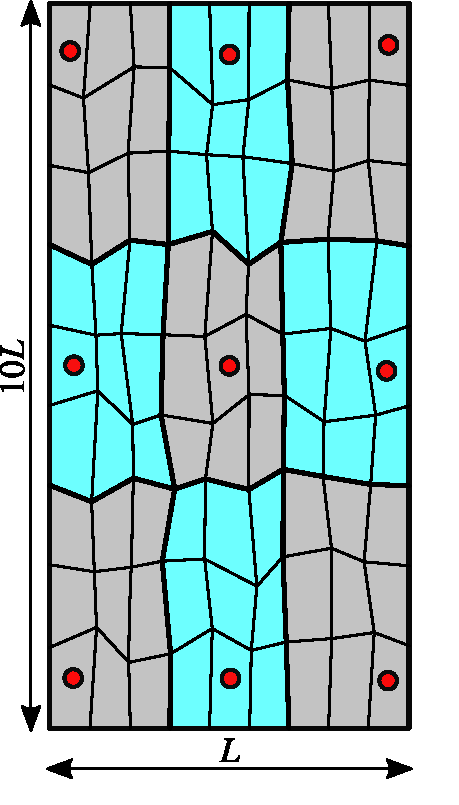
\includegraphics[width=\linewidth]{figs/MPFA_9x9_a}}
  \caption{\label{fig:mpfa_demo_grid}}
\end{subfigure}
\hfill
\begin{subfigure}[t]{0.22\textwidth}
  \centerline{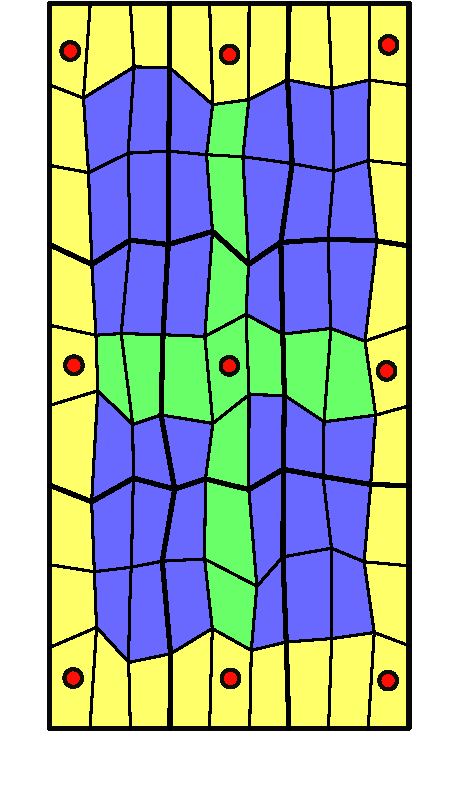
\includegraphics[width=\linewidth]{figs/MPFA_9x9_b}}
  \caption{\label{fig:mpfa_demo_support}}
\end{subfigure}
\hfill
\begin{subfigure}[t]{0.22\textwidth}
  \centerline{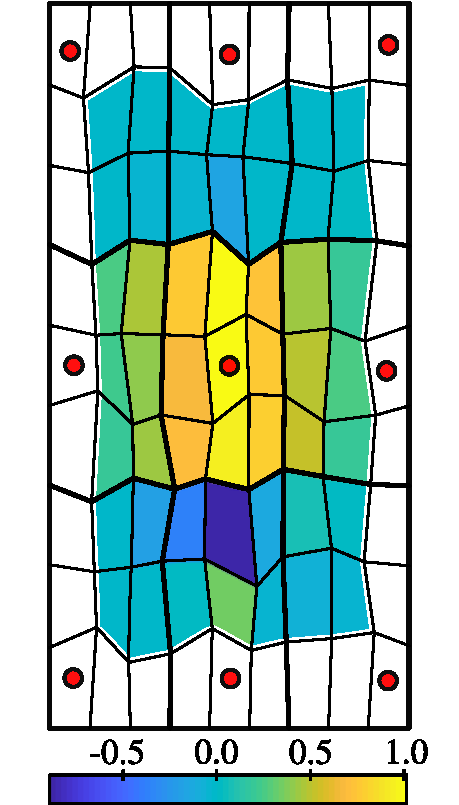
\includegraphics[width=\linewidth]{figs/MPFA_9x9_c}}
  \caption{\label{fig:mpfa_demo_orig}}
\end{subfigure}
\hfill
\begin{subfigure}[t]{0.22\textwidth}
  \centerline{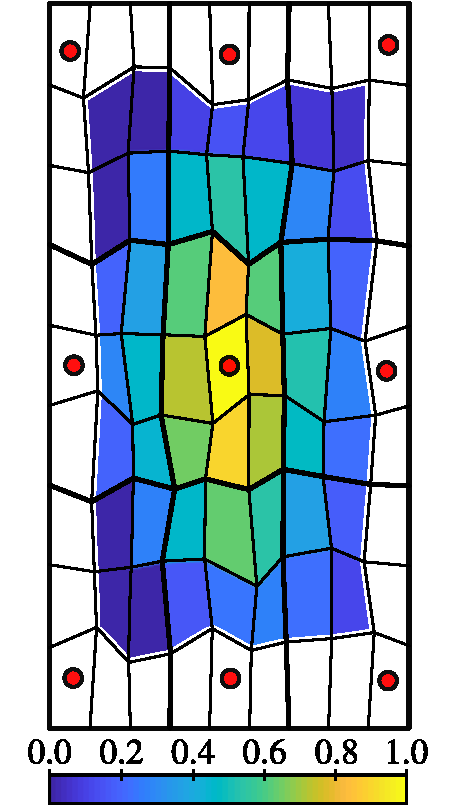
\includegraphics[width=\linewidth]{figs/MPFA_9x9_d}}
  \caption{\label{fig:mpfa_demo_alter}}
\end{subfigure}
\caption[MsRSB basis functions for MPFA flow problem]{\label{fig:mpfa_demo} Basis function for the center block of a regular 3$\times$3 partition: (a) primal grid and coarse nodes (\Colorcircle{red}); (b) support boundary (\Colorcircle{yellow}), edge (\Colorcircle{green}) and internal cells (\Colorcircle{blue}); (c) MsRSB basis function using the original fine-scale system; and (d) MsRSB basis function using the adjusted fine-scale system. The relative grid dimensions are not to scale.}
\end{figure}

To demonstrate the effect the approximation has on the smoothed basis iteration, we consider a simple test case shown in \autoref{fig:mpfa_demo}.   Starting from a regular $9 \times 9$ Cartesian square, we randomly perturb the vertex positions and then stretch the grid by a factor of 10 in the $y$-direction.   The resulting discrete system exhibits anisotropy in coefficients even with isotropic permeability tensor and deviates strongly from the TPFA approximation.   We consider a $3 \times 3$ coarse grid and employ MsRSB iteration to iteratively converge basis functions to a tight tolerance of $e_{it} = 10^{-12}$, monitoring the basis function associated with the central coarse cell.   Without any modification to the system matrix, the process begins to diverge after approximately 10 iterations, and basis functions become unphysical with negative pressure values, as displayed in \autoref{fig:mpfa_demo_orig}.   On the other hand, iteration based on a matrix filtered according to \eqref{eq:msrsb_mpfa_filtering} converges and results in the desired monotone basis functions, as evident from \autoref{fig:mpfa_demo_alter}.   Note that due to cancellation of several connections in the MPFA matrix, the basis function does not fully spread to the corners of its support region.   This does not present a problem in practice since the missing cells are still interpolated by other coarse pressures (it is impossible for all connections of a cell to be filtered out simultaneously) and partition of unity in the interpolation operator is preserved by construction.   Finally, we note that the treatment developed here for MPFA-O scheme is quite general and applies to other flavors of multi-point schemes, such as MPFA-L and MPFA-G, although conducting thorough testing with all of them is beyond the scope of this work.

\subsection{MsRSB for FEM Linear Elasticity}
\label{subsec:enhanced_msrsb_mech}

We further investigate the extension of matrix lumping ideas to preconditioning linear systems arising from finite element discretizations of second order elliptic PDEs with vector unknowns.   Considering the governing equation for quasi-static linear momentum balance in displacement formulation and assuming linear elastic behavior:
\begin{align}
    \nabla \cdot \tensorTwo{\sigma(\vec{u})} + \vec{b} &= 0 \\
    \tensorTwo{\sigma}(\vec{u}) &= \tensorFour{C} : \nabla^s \vec{u}
    \label{eq:elasticity_pde}
\end{align}
the discrete finite element linear system reads:
\begin{align}
    A^h\vec{u}^h = \vec{f}^h
\end{align}
where $A^h$ is the finite element global stiffness matrix, $\vec{u}^h$ is the discrete vector of displacement unknowns with $n_{sd}$ (the number of spatial dimension) unknowns per grid node, and $\vec{f}^h$ is the discrete forcing vector.   For exposition purposes only, we assume here that unknowns are ordered by each coordinate directions.   The stiffness matrix $A^h$ then possesses the block structure:
\begin{align}
	A^h &=
    \begin{bmatrix}
        A_{xx}^h & A_{xy}^h & A_{xz}^h \\
        A_{yx}^h & A_{yy}^h & A_{yz}^h \\
        A_{zx}^h & A_{zy}^h & A_{zz}^h 
	\end{bmatrix},
	\label{eq:blk_stiff}
\end{align}
where the off-diagonal blocks reflect the full coupling between $x$, $y$ and $z$ components (in two dimensions the number of blocks would be $2 \times 2$).   As an important aside, \eqref{eq:elasticity_pde} is not a purely elliptic equation, but rather is a system of $n_{sd}$ coupled elliptic PDEs.   Note that $A^h$ is symmetric positive definite (assuming Dirichlet boundary conditions, if any, are applied in a symmetry-preserving fashion), but is not an M-matrix in general.   This implies that a standard restricted smoothing iteration applied to $A^h$ would face the same divergence issue previously observed with MPFA.

To overcome this issue, we employ a two-step approximation of $A^h$.   First, the so-called separate displacement component (SDC) \cite{Gustafsson1996} approximation reads:
\begin{align}
	A^{\textsc{sdc}} &=
    \begin{bmatrix}
  	    A_{xx}^h &          &        \\
  	             & A_{yy}^h &        \\
  	             &          & A_{zz}^h 
	\end{bmatrix},
    \label{eq:blk_stiff_SDC}
\end{align}
i.e. a sparsification of $A^h$ that consists of discarding all cross-coupling terms between the vector unknowns.   The motivation behind SDC as a preconditioning approach is that the approximate matrix is spectrally equivalent to the full stiffness matrix \cite{Blaheta1994,Gustaffson1998}, yet is more sparse and decomposes the coupled problem into $n_{sd}$ independent elliptic problems that are much more favorable to existing preconditioning techniques, such as incomplete factorizations and multigrid methods.   More specifically, each diagonal block $A_{ii}$ corresponds to finite element discretization of an anisotropic diffusion operator \cite{Bosma2021}.   Note that this approximation breaks down in the incompressible elasticity limit (i.e. Poisson ratio $\nu \to 0.5$ \cite{Axelsson1978}), however this is of no concern for most problems of interest in subsurface poromechanics, where typical values lie in the range $0.1 \leq \nu \leq 0.4$.

The second approximation step consists of applying lumping technique developed for MPFA flow to the diagonal blocks of SDC stiffness matrix --- that is, we construct $\tilde{A}^h$ where each of the $n_{sd}$ diagonal blocks $\tilde{A}_{ii}^h$ is the result of applying \eqref{eq:msrsb_mpfa_filtering} to $A_{ii}^h$.   As a result, $\tilde{A}^h$ becomes a (weakly diagonally dominant) M-matrix suitable for smoothing iteration.   For the case of a stiffness matrix of scalar FEM with Neumann boundary conditions, \cite{Xu2017} contains a formal proof of spectral equivalence of $A_{ii}^h$ and $\tilde{A}_{ii}^h$ constructed in this fashion (referred to therein as an \textit{M-matrix relative} of $A_{ii}^h$).   By extension and due to SDC approximation, this implies spectral equivalence of the $A^{\textsc{sdc}}$ and $\tilde{A}^h$.   In addition, we once again note the similarity of our lumping approach to existing preconditioning techniques --- namely, the one introduced in \cite{Gustafsson1996} with the goal of ensuring existence and robustness of incomplete factorizations of the stiffness matrix.   While their lumping applied before assembly, at the level of individual element matrices, in present work it is performed on the assembled matrix, with similar end result.

In a FEM simulation of elasticity, $n_{sd}$ unknowns are collocated at each node of the mesh both at the fine and the coarse level, therefore each coarse node also has $n_{sd}$ coarse basis functions associated with it, one per coordinate direction.   Computing these functions based on $\tilde{A}^h$ which includes SDC approximation leads to fine-scale displacement field in each coordinate direction being expressed as a linear combination of coarse node displacements in that direction only.   The resulting interpolation operator $P$ is thus block-diagonal, which constitutes a major difference from a classic MsFE approach to geomechanics, which constructs fully coupled basis functions \cite{Castelletto2017} that account for additional coupling between all fine- and coarse-scale solution directions, at the cost of much denser basis functions.   However, despite the decoupled basis, MsRSB coarse-scale stiffness matrix $A^H = R A^h P = P^T A^h P$ is coupled, with each block computed via
\begin{align}
A^H_{ij} = P^T_{ii} A_{ij}^h P_{jj}, \quad i,j \in \{x,y,z\}
\end{align}
and thus still captures the interactions between components of displacement vector at the coarse scale (note that the original coupled stiffness matrix $A$ is used here).   On the other hand, use of SDC approximation offers the ability of construct basis functions associated with each coordinate direction separately, by performing smoothing iteration on each $\tilde{A}_{ii}$ and $P_{ii}$ independently.   This can lead to substantial computational savings if basis in some coordinate direction converges slower than in the others, avoiding needless updates to already converged blocks of $P$.   In practice, the user-provided matrix $A$ often has node-wise ordering, and there is additional work involved associated with permuting it into block form considered above and re-assembling the node-ordered prolongation operator from blocks $P_{ii}$, so one must weigh potential computational savings against these additional costs.

\begin{figure} [htbp]
\begin{subfigure}[t]{0.22\textwidth}
  \centerline{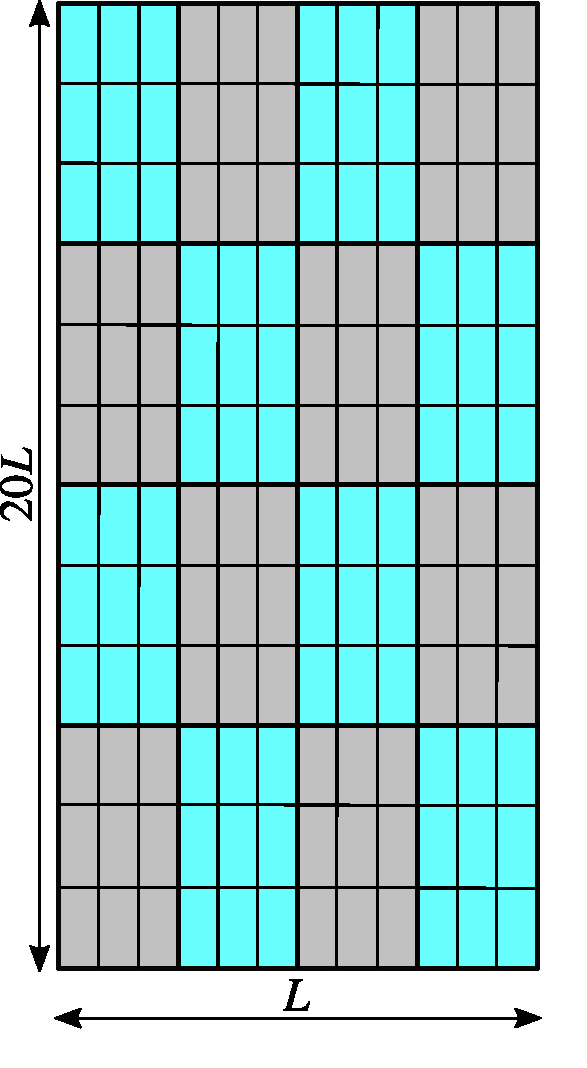
\includegraphics[width=\linewidth]{figs/FE_12x12_a}}
  \caption{\label{fig:fem_demo_grid}}
\end{subfigure}
\hfill
\begin{subfigure}[t]{0.22\textwidth}
  \centerline{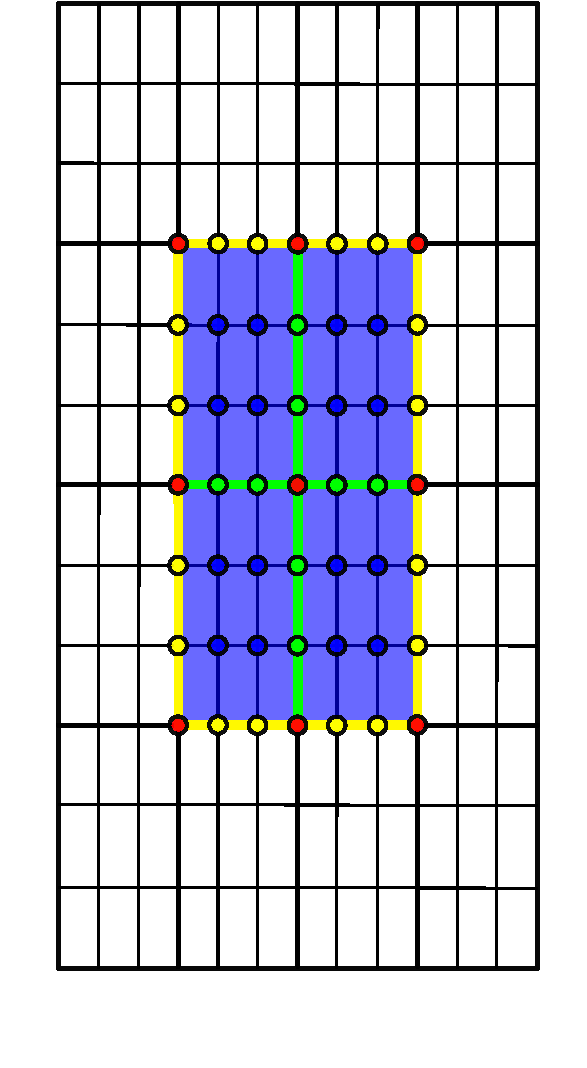
\includegraphics[width=\linewidth]{figs/FE_12x12_b}}
  \caption{\label{fig:fem_demo_support}}
\end{subfigure}
\hfill
\begin{subfigure}[t]{0.22\textwidth}
  \centerline{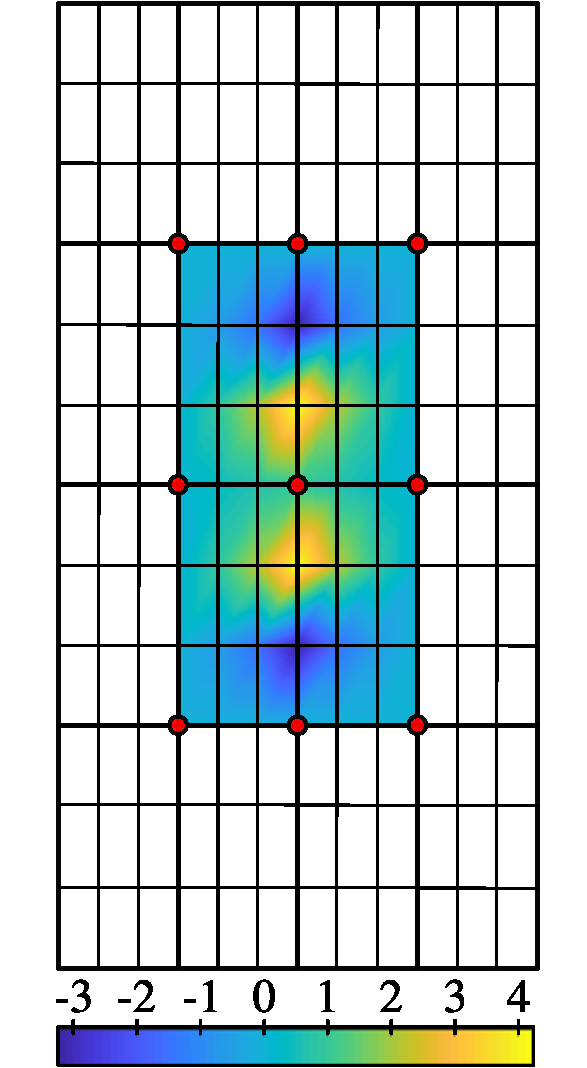
\includegraphics[width=\linewidth]{figs/FE_12x12_c}}
  \caption{\label{fig:fem_demo_orig}}
\end{subfigure}
\hfill
\begin{subfigure}[t]{0.22\textwidth}
  \centerline{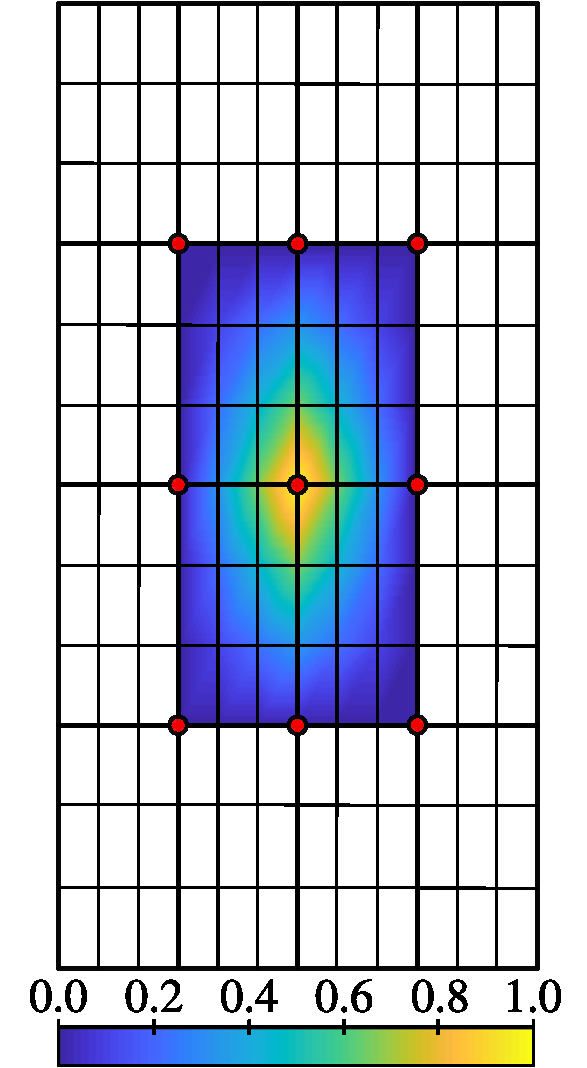
\includegraphics[width=\linewidth]{figs/FE_12x12_d}}
  \caption{\label{fig:fem_demo_alter}}
\end{subfigure}
\caption[MsRSB basis functions for FEM linear elasticity]{\label{fig:fem_demo} Basis function for $x$-displacement of the middle coarse node of a regular 4$\times$4 partition: (a) primal grid; (b) coarse (\Colorcircle{red}), support boundary (\Colorcircle{yellow}), edge (\Colorcircle{green}) and internal (\Colorcircle{blue}) nodes; (c) MsRSB basis function using the original fine-scale system; and (d) enhanced MsRSB basis function using the adjusted fine-scale system. The relative grid dimensions are not to scale.}
\end{figure}

This matrix lumping approach is demonstrated on a simple conceptual two-dimensional test case shown in \autoref{fig:fem_demo}, consisting of a simple homogeneous problem on a Cartesian $12 \times 12$ fine-scale grid defined in terms of dimensionless quantities with unit Lam\'{e} parameters.  The coarse grid is $4 \times 4$ with 5 nodes in each direction, and we are investigating the basis functions associated with the middle coarse node.   Unlike the MPFA test in \autoref{subsec:enhanced_msrsb_flow}, there is no need to perturb the grid nodes; it is sufficient to simply introduce anisotropy by stretching the grid (we used a factor of 20) along the $y$-axis to induce positive off-diagonal coefficients that violate M-matrix properties.   Basis iteration with original system matrix diverges after about 20 iterations, and the $x$-displacement basis function contains negative values, as shown in \autoref{fig:fem_demo_orig}.   On the other hand, iteration on the altered matrix converges (using a tolerance $e_{it} = 10^{-12}$) to the expected bilinear basis functions displayed in \autoref{fig:fem_demo_alter}.

To assess the effect of proposed matrix modifications on interpolation quality and performance of the preconditioner, we consider a two-dimensional test case from \cite{Castelletto2017}.   The test consists of a 2D elastic isotropic domain with a layered distribution of Young's modulus inspired by well log data and a constant Poisson ratio of 0.2.   The level of material contrast is controlled by parameter $\beta$ and varied between 1 and 3 orders of magnitude in Young's modulus variation.   Additionally, four mesh families are considered (\texttt{cart}, \texttt{skew}, \texttt{trig} and \texttt{rand}) each with a different type of geometric distortion applied to the coarse grid.   Each mesh consists of a base $7 \times 7$ Cartesian grid that is further refined by a factor into a $224 \times 224$ fine grid, from which several structured coarse grids are generated using varying coarsening ratios.   Finally, three types of boundary conditions are prescribed: two representing laterally constrained and unconstrained vertical compression respectively, and one representing simple shear in the $x$-direction.   For each combination of these parameters, a full preconditioned iterative solution is performed, replicating the solver setup used in \cite{Castelletto2017}: BiCGStab acceleration with two-stage multiscale preconditioning using two-level multiscale operator as the first (global) stage ILU(0) as the second stage (local) post-smoother.   Results are summarized in \autoref{tab:2D_structured_BICGSTAB_iter} which lists the Krylov iteration counts for MsRSB-based preconditioner.   Our observation is that for this wide range of scenarios, the MsRSB version performs robustly and yields a number of iterations comparable to MsFE (see \cite{Castelletto2017}), with a only a modest increase (about 20-30\%) for most cases, with the exception of laterally constrained case on \texttt{cart} mesh where MsFE interpolation is exact and thus leads to immediate convergence.   Therefore, the proposed approach to computing basis functions via restricted smoothing on an algebraically lumped stiffness matrix constitutes a solid basis for the development of a scalable multilevel preconditioning framework.

\begin{figure}[htbp]
    \centering
    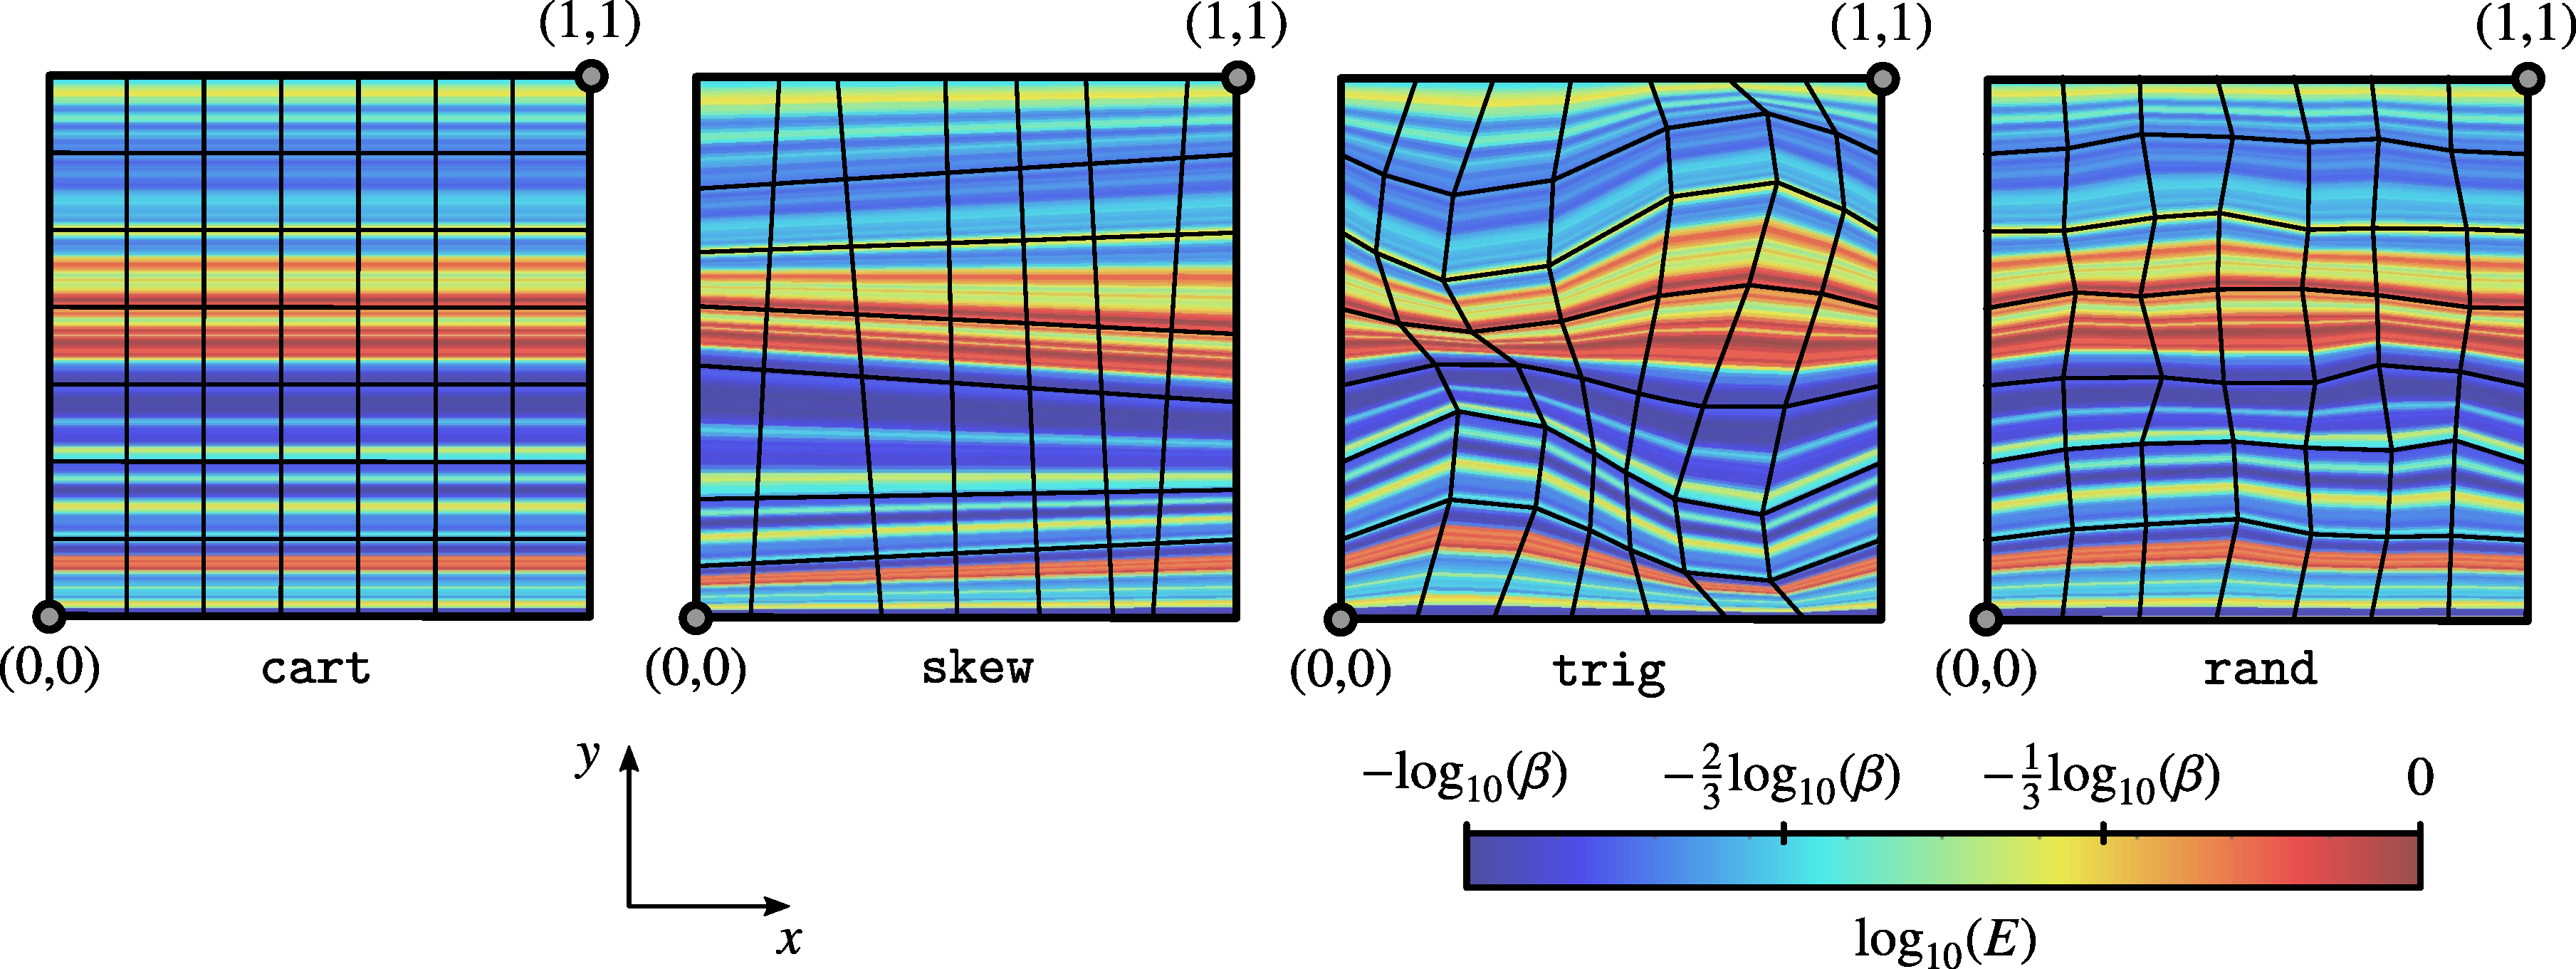
\includegraphics[width=\textwidth]{figs/2D_structured_young}
    \caption[Structured 2D heterogeneous geomechanics test case]{Structured 2D heterogeneous geomechanics test case: Young's modulus distribution and computational mesh setup.}
    \label{fig:2D_structured_young}
\end{figure}

\begin{table}
    \centering
    \caption[Structured 2D heterogeneous geomechanics test case: number of BiCGStab iterations]{Structured 2D heterogeneous geomechanics case: number of BiCGStab iterations to converge to $10^{-8}$ for different mesh families, coarse grid sizes and Young's modulus variations.}
    \label{tab:2D_structured_BICGSTAB_iter}
    \begin{small}
    \setlength\tabcolsep{3.8pt}
    \begin{tabular}{cccccccccccccccc}
        \hline\noalign{\smallskip}
        $\beta$ & \multirow{2}{*}{\begin{tabular}{c}\# coarse\\elements\end{tabular}} & \multicolumn{4}{c}{laterally constrained} & & \multicolumn{4}{c}{laterally unconstrained} & & \multicolumn{4}{c}{simple shear} \\
        \noalign{\smallskip}\cline{3-6} \cline{8-11} \cline{13-16}\noalign{\smallskip}
        & & \texttt{cart} & \texttt{skew} & \texttt{trig} & \texttt{rand} & & \texttt{cart} & \texttt{skew} & \texttt{trig} & \texttt{rand} & & \texttt{cart} & \texttt{skew} & \texttt{trig} & \texttt{rand} \\
        \hline\noalign{\smallskip}
        1 & $56\times56$ & 5 & 7 & 6 & 5 & & 4 & 7 & 6 & 5 & & 6 & 7 & 7 & 5 \\
          & $28\times28$ & 8 & 10 & 11 & 8 & & 8 & 12 & 11 & 10 & & 13 & 16 & 17 & 14 \\
          & $14\times14$ & 16 & 20 & 19 & 16 & & 18 & 21 & 22 & 19 & & 26 & 29 & 32 & 26 \\
          & $7 \times7 $ & 37 & 33 & 40 & 40 & & 41 & 38 & 43 & 43 & & 40 & 47 & 44 & 42 \\
        \hline\noalign{\smallskip}
        2 & $56\times56$ & 4 & 6 & 6 & 5 & & 5 & 6 & 6 & 6 & & 5 & 6 & 6.5 & 5 \\
          & $28\times28$ & 7 & 10 & 12 & 8 & & 9 & 10 & 12 & 9 & & 12 & 19 & 20 & 17 \\
          & $14\times14$ & 17 & 26 & 26 & 18 & & 18 & 23 & 25 & 22 & & 37 & 39 & 46 & 37 \\
          & $7 \times7 $ & 46 & 50 & 54 & 49 & & 52 & 58 & 53 & 53 & & 51 & 59 & 55 & 51 \\
        \hline\noalign{\smallskip}
        3 & $56\times56$ & 4 & 6 & 8 & 6 & & 6 & 8 & 10 & 9 & & 6 & 7 & 8 & 7 \\
          & $28\times28$ & 10 & 11 & 13 & 10 & & 11 & 12 & 17 & 10 & & 17 & 19 & 19 & 18 \\
          & $14\times14$ & 22 & 30 & 39 & 30 & & 21 & 32 & 40 & 34 & & 46 & 49 & 47 & 50 \\
          & $7 \times7 $ & 49 & 61 & 73 & 63 & & 63 & 71 & 86 & 71 & & 62 & 67 & 71 & 58 \\
        \hline\noalign{\smallskip}
    \end{tabular}
    \end{small}
\end{table}

% ===================== SECTION =====================
\section{Multilevel Coarsening for General Polyhedral Grids}
\label{sec:msrsb_coarsening} 

\subsection{Grid Representation}
\label{subsec:msrsb_coarsening_grid}

Definition of any multiscale method starts with the selection of a coarse grid (or a sequence of them).   Historically many multiscale methods have been designed and validated primarily with relatively simple topologies (which we understand as the connectivity structure of grid vertices and cells), such as structured Cartesian.   Such grids are both preferred by academic researchers due to ease of use and clarity of presentation, and employed widely in industrial numerical modeling workflows, owing to the efficiency, robustness and accuracy of most discretizations and solvers and such grids.   In many methods, the requirement of structured topology of the coarse grid is not stated explicitly, but implied.   For example, in MsFE the need to assemble reduced boundary problems along coarse-scale interfaces (faces, and in 3D also edges) generally assumes that the coarse interface have regular well-behaved shapes --- faces are expected to be more or less flat surfaces and edges straight lines, otherwise constructing tangential operator projections such as $\nabla_{\parallel}$ onto a reduced-dimension space requires potentially much less accurate approximations of fine-scale behavior, leading to lower quality interpolation and slower convergence of the scheme.   Moreover, the challenge of constructing a coarse grid in a completely unstructured three-dimensional setting has not been systematically addressed.   This is reasonable, as the method was devised as a way of solving a finite-element problem at the coarse scale, with sub-grid resolution provided by numeric multiscale shape functions, and finite-element methods primarily deal with well-defined element shapes.   Multiscale Mixed Finite Element (MsMFE) method \cite{Chen2002} addresses the geometric flexibility issue of MsFE by replacing local Dirichlet problems with Neumann problems used to obtain velocity basis functions.   This allowed the method to be used on grids with complex stratigraphy and topology \cite{Aarnes2008,Alpak2012}; however the fine-scale problem is assumed to be written in the mixed form, which is not the case for most simulation workflows.

On the other hand, MsFV method allow for a much more flexible algebraic construction of the reduced boundary problems \cite{Wang2014}, but leans heavily on the primal-dual partitioning of the grid.   While relatively straightforward to construct for structured and semi-structured topologies, robust dial partitions are difficult or sometimes impossible to achieve in an automatic manner for a wide range of coarsening ratios \cite{Moyner2014a}.   Graph-based algorithms have been employed to overcome some of these issues \cite{Mehrdoost2019}, but remain largely limited to two-dimensional problems, due to the complexity of defining three-dimensional faces in arbitrary topologies.   MsTPFA method addresses these shortcomings by combining two-point basis functions computed on the primal coarse grid with specially constructed numerical partition of unity functions that glue together flow solutions associated with coarse interfaces \cite{Moyner2014}.   While it admits coarse grids with cells represented by arbitrary disjoint partitions of fine cells, the method itself if quite complicated to implement.   Finally, MsRSB method described in \autoref{subsec:related_work_msrsb} provides a similar level of grid flexibility, but involves a construction of support regions based on geometric triangulation of local neighborhoods of each coarse cell, requiring to carry geometric properties (at the very least, cell and face centroids) not only at the fine level, but also at every coarse level if the method is to be applied in a multilevel fashion.   Naturally, all of these methods focus on cell-centered variables exclusively, and do not address the issue of nodal degrees-of-freedom used in finite-element problems.

Our goal is to adopt a multilevel mesh representation suitable for both flow and mechanics and devise the associated algorithms for constructing a sequence of coarser meshes.   The minimum requirements for the mesh data structure are:
\begin{itemize}
    \item must provide a way to coarsen both cells and nodes of the fine grid;
    \item must have identical representation at each level, allowing for recursive coarsening;
    \item must be as ''algebraic'' as possible (not involve any geometric data).
\end{itemize}
This last requirement is particularly interesting.   Purely algebraic methods are highly desirable in the world of solvers, since they aid in modularizing the code, minimizing the amount of data that needs to passed through an interface, and decoupling the linear solver from meshing, discretization and physics packages.   This is less important when multiscale method is used as an approximate solver that the rest of the software package is built around, but paramount when it is one of several acceleration option for the solution of linear systems (i.e. a preconditioner or a building block for one).   Black-box methods are highly desirable in numerical software, and Algebraic Multigrid (AMG) preconditioners have achieved a lot of success in part due to their flexibility and simple interface that, at minimum, only requires the system matrix to be provided.   However even AMG packages typically offer a way for the user to provide additional information about the degrees-of-freedom, such as their types or collocation in space. For example the popular SAMG \cite{?} library allows the user to specify a vector of degree-of-freedom labels indicating their type or physical space point they belong to, which allows the solver to make optimal choices with regard to coarsening and smoothing.   Similarly, algebraic MsFV solvers require either knowledge of the grid to construct the primal-dual partitioning, or at least access to the user-provided ''wirebasket'' classification of fine-scale cells.

Given the aforementioned requirements, we define a grid level as:
\begin{itemize}
    \item a set $V_N$ of $|V_N| = N_N$ nodes (vertices) as abstract points in $n_{sd}$-dimensional space (coordinates or any other physical attributes are not used);
    \item a set $V_E$ of $|V_E| = N_E$ of elements (cells) as abstract volumes in $n_{sd}$-dimensional space (no assumptions are made about convexity or any specific shape, including being a polytope);
    \item a set $V_B, |V_B| = N_B$ of global domain boundaries;
    \item element-to-node topology described through its bipartite directed graph $\mathcal{G}_E = (V_E,V_N,E_E)$ or, equivalently, sparse adjacency matrix $\mathcal{A}_{E} \in \set{0,1}^{N_E \times N_N}$, $[\mathcal{A}_E]_{ij} = 1 \Leftrightarrow (i,j) \in E_E$;
    \item domain boundary-to-node map defined by its bipartite directed graph $\mathcal{G}_B = (V_B,V_N,E_B)$ or sparse matrix $\mathcal{A}_{B} \in \set{0,1}^{N_B \times N_N}$, $[\mathcal{A}_B]_{ij} = 1 \Leftrightarrow (i,j) \in E_B$.
\end{itemize}
Note that finite element terminology (nodes and elements) will be used interchangeably with generic mesh entity names (vertices and cells) where appropriate without confusion.   The need for preserving domain boundary indicators in the mesh description will be fully explained in \autoref{subsec:msrsb_coarsening_algorithm}; briefly speaking, they aid in increasing interpolation quality near the boundaries by placing more coarse nodes or shifting coarse cell centers near the boundary, which is key to accurate interpolation of boundary conditions.   A rectangular domain will have $2n_{sd}$ boundaries, but in general an arbitrarily-shaped domain could have any number of user-specified external surfaces.   As for element-to-node adjacency, this data is typically freely available in finite-element codes, since the element integration loop needs to assemble local element stiffness matrices into the global stiffness matrix, which requires mapping each element to its nodes (or corresponding degrees-of-freedom).   In addition, in a coupled FE-FV simulation, the sparsity structure of the coupling blocks $B_1$ and $B_2$ corresponds exactly to the element-to-node map (after taking into account unknown multiplicity, e.g. amalgamating rows/columns corresponding to $n_{sd}$ collocated displacement degrees-of-freedom).   In all other cases, the topological information must be provided explicitly by the simulation code.

A coarse grid is defined on top of a fine grid as follows (from here on, $h$ is used to refer to fine level objects/quantities and distinguish it from coarse level labeled $H$).
\begin{itemize}
    \item Coarse elements are formed by a non-overlapping partitioning (agglomeration) of fine-scale elements; this is represented by a partitioning vector $\vec{z}_E^h \in [1,N_E^H]^{N_E^h}$ at the fine scale.
    \item Coarse nodes are a subset of fine nodes located at intersections of multiple coarse cells (or more generally, subdomains). \autoref{subsec:msrsb_coarsening_algorithm} will detail exactly how this subset is chosen; this is represented by a mapping vector $\vec{z}_N^H \in [1,N_N^h]^{N_N^H}$.
    \item The set of domain boundaries is preserved at each level.
    \item Coarse element-to-node adjacency graph $\mathcal{G}_E^H$ is obtained by collapsing ''element'' nodes of $\mathcal{G}_E^h$ according to $\vec{z}_E^h$ and selecting a subset of ''vertex'' nodes according to $\vec{z}_N^H$.
    \item Coarse boundary-to-node map $\mathcal{G}_B^H$ is similarly obtained by selecting ''vertex'' nodes of $\mathcal{G}_B^h$ according to $\vec{z}_N^H$.
\end{itemize}
This definition follows a classical cell-based agglomeration approach, although other options are available (for example, based on nodal agglomerates).   This is convenient because material properties are usually assigned to each cell in the grid and thus can be used to influence the coarsening process.   In a parallel setting, it is convenient to have coarse partition boundaries match the process subdomain boundaries, as explained in \autoref{ch:parallel_multiscale}.   \autoref{fig:square_coarse} shows an example of a coarse grid obtained by agglomeration (partitioning) of fine cells of an unstructured 2D triangle grid.

\begin{figure}[htbp]
  \begin{subfigure}[t]{0.5\textwidth}
    \centerline{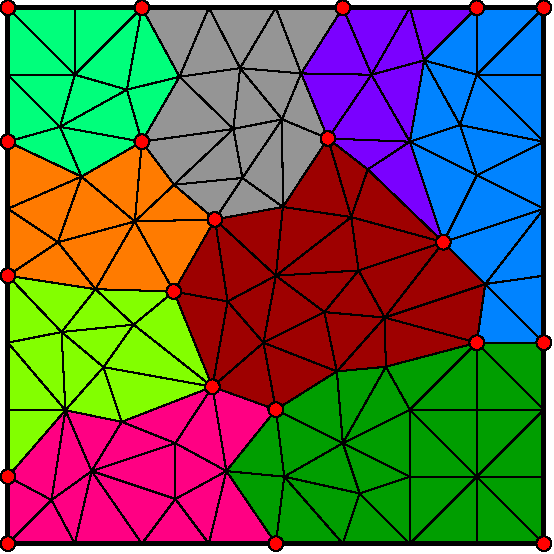
\includegraphics[width=0.6\linewidth]{figs/square_tria_coarse}}
  \end{subfigure}
  \begin{subfigure}[t]{0.5\textwidth}
    \centerline{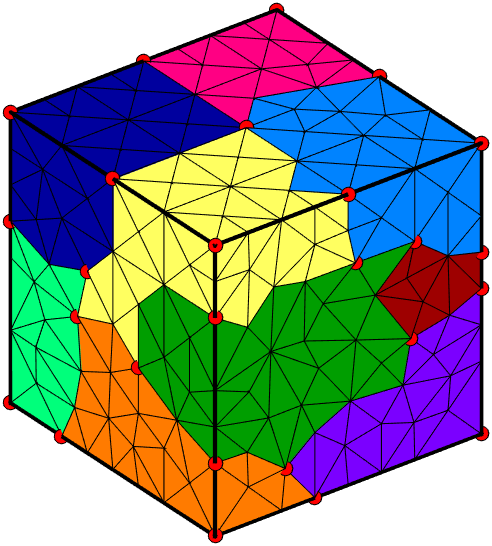
\includegraphics[width=0.6\linewidth]{figs/cube_tetra_coarse}}
  \end{subfigure}
  \caption[Unstructured coarse grid examples]{\label{fig:square_coarse} Example of unstructured coarse grid in 2D (left) and 3D (right). Cell colors correspond to coarse cells (partitions) and coarse nodes are marked (\Colorcircle{red})}
\end{figure}

\subsection{Coarsening Algorithm}
\label{subsec:msrsb_coarsening_algorithm}

\subsubsection{Cell Partitioning}

The first step in generating a coarse grid at any level is to construct the cell partitioning vector, $\vec{z}_E^h$.   This is typically achieved using a variety of methods:
\begin{itemize}
    \item Geometrical coarsening, such as recursive inertial bisection (RIB) or space filling curves. These require cell centroid information to be preserved/computed at each level, which is not desirable in a practical implementation.   In our prototype implementation RIB option is available for comparison purposes only.
    \item (Semi-)structured coarsening, such as Cartesian coarsening of a topologically Cartesian fine grid.   Another example is 2.5D grid coarsening, in which the unstructured surface grid is partitioned using any appropriate method, and vertical layers are partitioned in a structured way according to structured layer index.   These methods require some additional structural information ($ijk$-index or column/layer index of each cell) to be available at each level either explicitly or implicitly , but they generally result in higher quality partitions.   In addition, they enable the use of semi-coarsening (coarsening preferentially in a particular direction) which is often advantageous for problems with strong mesh or material anisotropy.
    \item Unstructured topological coarsening, for example using a graph partitioning algorithm such as k-way partitioning or recursive bisection, often accessed though software packages such as METIS \cite{Karypis1999} or Scotch \cite{Chevalier2008}.   These algorithms offer the utmost flexibility with respect to grid topology.   Input cell connectivity graph $\mathcal{G}_C^h$ is constructed based on mesh topology description $\mathcal{G}_E^h$.   This can be formally expressed as computing a \textit{bipartite half-square} of $\mathcal{G}_E^h$ (omitting superscript $h$ for ease of notation):
    \begin{align}
        \mathcal{G}_C &= \mathcal{G}_E^2[V_E] = (V_E,E_E^2) \label{eq:graph_square}\\
        E_E^2 &= \set{(e_i,e_j) \bigm| \exists n_k \in V_N: (e_i,n_k) \in \mathcal{G}_E, (e_j,n_k) \in \mathcal{G}_E} \label{eq:graph_square_edges}
    \end{align}
    In addition, it might be desirable to limit the cell graph to a subset of edges that only connect cells sharing a face (to mimic TPFA connectivity pattern).   This is achieved by weighting edges in $E_E^2$ according to the number of shared nodes $n_k$ in \eqref{eq:graph_square_edges} and removing edges with weight below $n_{sd}$.   For problems with scalar cell-centered unknowns, graph edges can be weighted according to the scale of off-diagonal entries in the fine-scale system matrix which reflect the level of material contrast and thus can adapt the coarsening to various physical features such as channels, faults and flow barriers, which proves highly beneficial in real-world models with high permeability contrast \cite{Klemetsdal2020}.   We use the following edge weighting scheme slightly modified from one previously proposed in the context of domain decomposition preconditioning \cite{Vecharynski2014}:
    \begin{align}
        w_{ij} = \gamma \frac{|a_{ij} + a_{ji}|}{2\sqrt{a_{ii} a_{jj}}} \label{eq:graph_matrix_weights}
    \end{align}
    with $\gamma$ a sufficiently large value required to represent weights as integer values as expected by many software packages.    Finally, graph partitioning methods offer a large number of options controlling partition quality, balancing and other aspects of algorithm behavior.   Advanced variants such as multilevel tabu search algorithm with local adaptation to permeability field \cite{Mehrdoost2019} have been applied to achieve improved quality coarse partitions that avoid non-convex cell shapes and high material contrast along coarse cell boundaries.
\end{itemize}

A key parameter in the coarsening process is the (cell-based) \textit{coarsening ratio} $C_r$ representing the average number of fine cells per coarse cell:
\begin{align}
    C_r = \frac{N_E^h}{N_E^H}
\end{align}
We will distinguish it from \textit{effective} (unknown-based) coarsening ratio $C_r^d$:
\begin{align}
    C_r^d = \frac{N_d^h}{N_d^H}
\end{align}
where $N_d$ is the number of degrees-of-freedom at the corresponding level. The two coincide in case of problems with cell-centered unknowns, but can be substantially different for nodal degrees-of-freedom (and consequently, for coupled problems with both unknown types). In examples using (semi-)structured coarsening, we will sometimes use a Cartesian coarsening ratio definition ($C_r = C_r^x \times C_r^y \times C_r^z$) or 2.5D coarsening ratio ($C_r = C_r^a \times C_r^z$) for convenience. Coarsening ratios can vary several orders of magnitude, but typically multiscale methods tend to avoid very small ones ($C_r < 4^{n_{sd}}$).

\subsubsection{Coarse Node Selection}

Once coarse cells are defined, coarse nodes must be determined by selecting a representative set of fine-scale nodes.   This problem is not well defined: while it's obvious which nodes should be transferred to the coarse level in case of structured partitioning (typically, a subset of nodes along each coordinate direction with a fixed step corresponding to the Cartesian coarsening ratio in that direction), the answer is less obvious for unstructured coarsening.   Extending the analogy from finest-scale grid, we can define a \textit{coarse face} as the union of fine faces shared by exactly two coarse cells.   Similarly, a \textit{coarse edge} is a union of line segments (fine edges) shared by a group of at least $n_{sd}$ coarse cells.   In two dimensions, coarse edges and coarse faces naturally coincide, which therefore suggests a very simple algorithm for determining coarse nodes: any fine node adjacent to three or more coarse cells becomes a coarse node.   To account for domain boundaries, the above definition can be extended to use coarse \textit{subdomains} instead, where a subdomain is either a real coarse cell or a virtual one extending outside the physical domain.   In practice, it is sufficient to introduce a single virtual coarse subdomain per uniquely identified domain boundary.   This has the effect of placing an additional coarse node at the junction of two coarse cells and a domain boundary, or two boundaries and a single coarse cell; \autoref{fig:square_coarse} demonstrates this in two dimensions.   Additional coarse nodes and corresponding coarse degrees of freedom improve interpolation quality near the boundary, which is especially important if Dirichlet boundary conditions are applied (this is almost always the case for domain boundaries in mechanics problems).

The above criterion does not generalize well to three dimensions.   Indeed, it's easy to see that an arbitrary number of coarse cells can conjoin on a group of fine nodes forming a coarse edge, but only the endpoints of the edge should be marked as coarse nodes.   To generalize this idea to arbitrary topologies, we propose an adaptation of hierarchical graph decomposition algorithm \cite{Henon2006}.   In their work, mesh nodes are grouped into \textit{connectors} according to mesh graph partition adjacency, and the algorithm builds a hierarchy of connectors optimal in some sense at every level of decomposition, with the aim of performing work (computing ILU factors) on decoupled subsets of the mesh in parallel.   In contrast, in this work we are interested in finding highest-level connectors (i.e. coarse nodes) only.   The algorithm thus proceeds as follows:
\begin{enumerate}
    \item Coarse subdomains are defined by adding each global domain boundary as a new ''virtual'' subdomain.   The number of subdomains is $N_S^H = N_E^H + N_B$, and for convenience, coarse cell subdomain numbering is preserved and virtual subdomains are assigned new indices $N_E^H+1,\ldots,N_E^H+N_B$.
    \item Subdomain-to-fine node adjacency graph $\mathcal{G}_S$ is built by collapsing element vertices of $\mathcal{G}_E^h$ that have the same partition index $\vec{z}_E^h$ and taking a union with $\mathcal{G}_B^h$ (with graph vertices appropriately renumbered). 
    \item Each fine-scale node $i \in [1,N_N^h]$ is assigned a \textit{key} $K_i$ consisting of the indices of adjacent coarse subdomains:
    \begin{align}
        K_i = \Set{ k \in [1,N_S^H] \bigm| (k,i) \in \mathcal{G}_S }
    \end{align}
    \item Nodes that share the same key are grouped together into a \textit{feature} (or connector).   This is represented by nodal grouping vector $\vec{z}_F^h \in [1,N_F]^{N_N^h}$, with $N_F$ the total number of features.   In practice, nodes that belong to the interior of a coarse cell or the interface between two subdomains (i.e. those with key cardinality $|K_i|$ of 1 or 2) can be discarded at this stage, so that only the ''edge skeleton'' of the mesh is remaining.
    \item A feature adjacency graph $\mathcal{G}_F$ is constructed by exploiting the fine-scale element-node adjacency information:
    \begin{align}
        \mathcal{G}_F = \set{(f_i,f_j) \bigm| \exists e \in [1,N_E^h], n_k, n_l \in [1,N_N^h]: (e,n_k), (e,n_l) \in \mathcal{G}_E^h, [\vec{z}_F^h]_k = i, [\vec{z}_F^h]_l = j}
    \end{align}
    In other words, two features are adjacent if any of their nodes are adjacent through a shared element at the fine scale.   The graph doesn't have to be computed explicitly, neighbor feature lists may be constructed dynamically on demand from the source data.
    \item Any feature $j$ whose key is fully subsumed by one of its immediate neighbors ($K_j \subset K_i, (i,j) \in \mathcal{G}_F$) is removed from the candidate set.   This simple criterion is the key simplification of the iterative multi-level decomposition procedure of \cite{Henon2006}.
    \item All remaining features are become coarse nodes.   Typically, each highest-level connector will only consist of a single fine-scale node, but on rare occasions multiple nodes are possible; in that case any one fine-scale node can be selected to represent the coarse node.
\end{enumerate}

\begin{figure}[htbp]
  \centerline{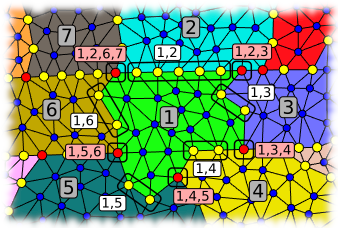
\includegraphics[width=0.5\linewidth]{figs/coarsening_2d_zoom_labels.png}}
  \caption[Coarse node selection algorithm example in 2D]{\label{fig:coarse_nodes_algo_zoom} Example of coarse node selection algorithm in 2D. Coarse subdomain indices shown in gray labels; coarse edge feature keys in white; coarse node feature keys in pink. Detected coarse nodes are marked (\Colorcircle{red}), edge nodes (\Colorcircle{yellow}); interior nodes (\Colorcircle{blue}). Groups of nodes representing connectors are outlined by black rounded borders.}
\end{figure}

The above algorithm works robustly for two- and three-dimensional grids with arbitrary topologies, as long as coarse cells are formed by contiguous partitions.   An example of its application is shown in \autoref{fig:coarse_nodes_algo_zoom} for a 2D grid for simplicity of visual presentation.   Focusing on interface nodes adjacent to coarse cell 1 and one of its neighboring cells, one can observe that the most natural choice of coarse nodes are those with the (locally) largest adjacency.   Note that this choice of nodes is not necessarily unique or optimal, but we find that in practice it strikes a good balance between representation quality and preserving acceptable coarsening ratio and operator density in a multilevel hierarchy.   Occasionally, the algorithm may lead to appearance of clusters of closely located or even directly adjacent coarse nodes (an example is visible is \autoref{fig:coarse_nodes_algo_zoom}). Even though this does not present a problem for the construction of the interpolation operator, it leads to suboptimal use of memory and computational power.   These cases may be addressed by merging multiple coarse nodes into one and adjusting coarse-scale topology maps accordingly.   We note that while the algorithm is sensitive to the quality of fine-scale cell agglomeration (in the sense of minimizing the unfavorable coarse cell shapes and coarse node clustering), the issue of optimal mesh partitioning is beyond the scope of present work.   Finally, we remark that the coarsening procedure may be applied recursively, since it relies only on cell-node and boundary-node adjacency maps that are constructed at each level.   Typical the multilevel preconditioner will proceed with the above algorithm to construct a grid hierarchy until a problem of sufficiently small size is obtained that is amenable to a direct solve.   Alternatively, it may be configured to construct a fixed number of levels, after which a different scalable solver such as AMG is invoked to solve (exactly or approximately) the coarsest level system.

% ===================== SECTION =====================
\section{Interpolation Operators}
\label{sec:msrsb_interpolation} 

Constructing the interpolation operator using MsRSB procedure involves the following steps:
\begin{enumerate}
    \item \label{itm:msrsb_step_matrix} Compute the Jacobi iteration matrix $G = I - \omega D^{-1} \tilde{A}$.
    \item \label{itm:msrsb_step_support} Construct the support region of each basis function, i.e. the set of points $I_j$ where basis function takes nonzero values:
    \begin{align}
        i \in I_j \iff P_{ij} \neq 0
    \end{align}
    \item \label{itm:msrsb_step_boundaries} Determine the support boundary sets $B_j$ and the union (global) boundary set $U = \bigcup\limits_{j} B_j$.
    \item \label{itm:msrsb_step_initp} Compute an initial (tentative) prolongation operator $P^0$.
    \item \label{itm:msrsb_step_iterate} Iterate until convergence according to \eqref{eq:msrsb_update}-\eqref{eq:msrsb_check}.
\end{enumerate}
Next, the steps 2--4 above are considered in detail for nodal and cell-centered basis functions. The remaining two steps can be implemented generally using algebraic operations on matrices for any type of interpolation operator.

\subsection{Nodal Basis Functions}
\label{subsec:msrsb_nodal_basis}

We begin by defining for each basis function is support, or area of influence.   Similar to the support of a regular fine-scale FEM shape function, the support of a basis function associated with a coarse node is defined to consist of the interior of the volume formed by the union of adjacent coarse subdomains.   More specifically, $I_j$ is the set of fine-scale nodes contained completely within the union of coarse subdomains incident on that coarse node.   These include both nodes completely interior to a single subdomain as well as those shared by several subdomains within support region (but none outside the support).   Virtual subdomains formed by global boundaries don't have any interior volume and consist purely of the corresponding boundary fine-scale nodes.   Their inclusion in the above definition is important, since it allows a basis function associated with a coarse node located on the boundary to take nonzero values and provide interpolation along that boundary.   Support boundary $B_j$ is identified to be the set of fine nodes adjacent to at least one coarse cell in support as well as at least one subdomain outside of support of coarse node $j$.   Alternatively, $B_j$ can be described as the set of fine nodes sharing a common fine cell with nodes in $I_j$ but not themselves belonging to $I_j$.   Both of these sets can be constructed in a fairly straightforward manner using adjacency graphs $\mathcal{G}_E^H$, $\mathcal{G}_E^h$ and partitioning vector $\vec{z}_E^h$.   Global sets $B$ and $I$ are then obtained with simple set union and difference operations.   \autoref{fig:square_node_supp} shows examples of nodal basis function supports with different types of meshes/partitioning (limited to 2D meshes for clarity).

\begin{figure}[htbp]
  \begin{subfigure}[t]{0.3\textwidth}
    \centerline{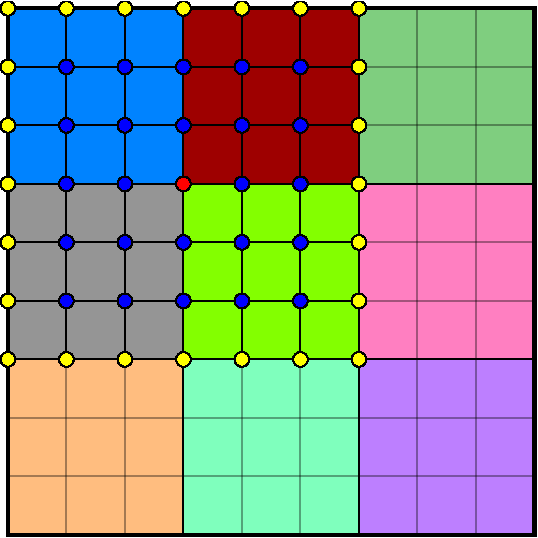
\includegraphics[width=0.9\linewidth]{figs/square_cart_struct_node_supp}}
  \end{subfigure}
  \hfill
  \begin{subfigure}[t]{0.3\textwidth}
    \centerline{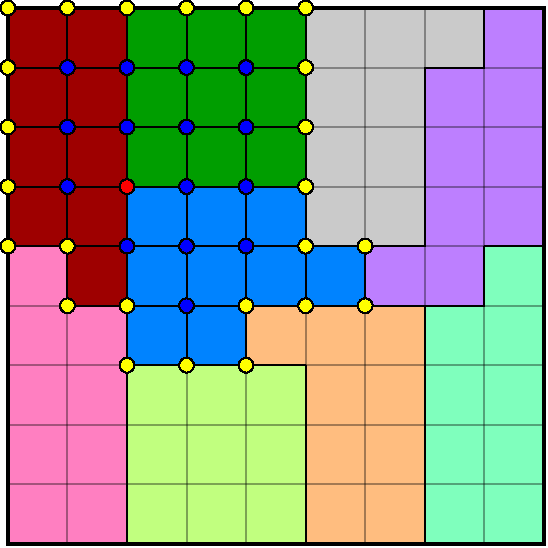
\includegraphics[width=0.9\linewidth]{figs/square_cart_metis_node_supp}}
  \end{subfigure}
  \hfill
  \begin{subfigure}[t]{0.3\textwidth}
    \centerline{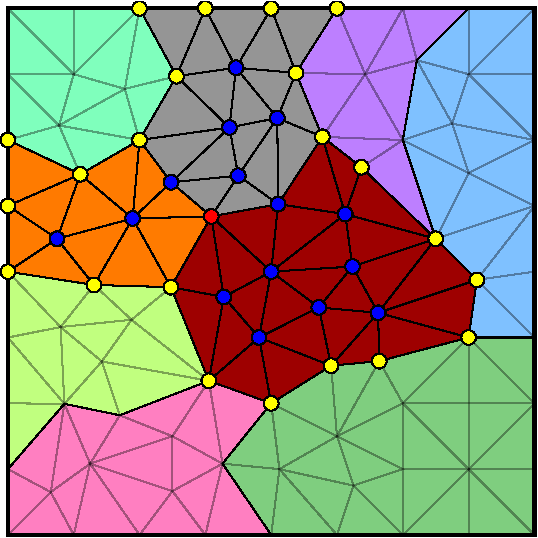
\includegraphics[width=0.9\linewidth]{figs/square_tria_metis_node_supp}}
  \end{subfigure}
  \caption[Nodal basis function support grid examples]{\label{fig:square_node_supp} Example of basis function supports (\Colorcircle{blue}) and support boundaries (\Colorcircle{yellow}) associated with a coarse node (\Colorcircle{red}) for different types of grids/coarsening: fully structured (left), graph-coarsened structured (middle) and fully unstructured (right).   The coarsening ratios are intentionally chosen to be small to simplify presentation.}
\end{figure}

Initial MsRSB prolongation operator assigns, for each basis function, a value of 1 to nodes in some vicinity of the corresponding coarse node and 0 to all others. Since the initial prolongation must satisfy partition of unity, each node must be assigned 1 by exactly one basis function, which naturally forms a non-overlapping partitioning of fine nodes. Unlike in the original cell-centered MsRSB method \cite{Moyner2016}, this partitioning for nodes is not available from the coarse grid hierarchy and must be constructed separately.   We propose the following node segmentation algorithm using topological adjacency data:
\begin{enumerate}
    \item Seed each partition with a single fine node corresponding to the associated coarse node.
    \item For each partition, compute the candidate set of new nodes by collecting the topological neighbors of nodes already in partition.   Neighbors are located via the nodal connectivity graph $\mathcal{G}_N = \mathcal{G}_E^2[V_N]$ that may be computed explicitly or implicitly.
    \item Exclude from the candidate set nodes that are already assigned to a partition, as well as any nodes that are not in support of the associated coarse node's basis functions (this prevents initial basis functions from accidentally extending beyond their prescribed support).
    \item If a node is assigned to more than one candidate set, choose only one and remove from all others.   The criteria for choosing the assignment may vary; examples that work well in practice include minimizing topological distance to the partition center (coarse node) or maximizing topological connectivity (number of neighbors in each partition).
    \item Merge candidate sets into their respective partitions and repeat steps 2--5 until no unassigned nodes remain.
\end{enumerate}

\autoref{fig:square_node_basis} demonstrates examples of generated nodal partitions on different types of grids/coarsening along with select initial and fully converged basis functions corresponding to each case (coarse nodes with non-overlapping support are chosen to improve visibility).   The converged basis function always spreads from each initial configuration to cover all the nodes in its support, as long as sufficient number of smoothing iterations are performed.   Note that in these examples the matrix used to construct the basis functions does not include the effects of boundary conditions.   In a typical simulation, however, this matrix is not available and instead the full system Jacobian with boundary conditions is provided to the linear solver.   Of the boundary conditions commonly used in mechanical problems, only boundary conditions of Dirichlet type have an effect on matrix, resulting in rows corresponding to constrained degrees-of-freedom containing just the diagonal element.   This has a clearly visible effect on the converged basis functions, showcased in \autoref{fig:square_node_bc}, particularly in the case of symmetric application of boundary conditions when the corresponding column is also zeroed out, resulting in a degree-of-freedom completely decoupled from the rest of the system.   As a consequence, basis functions centered on boundary nodes and associated with normal direction of that boundary end up interpolating only nodes along that boundary.   In practice this leads to only a small reduction in interpolation quality and a minor increase in overall Krylov iteration count, due to the action of smoothers that help reduce highly localized  errors associated with boundary conditions.   Note that symmetric application of Dirichlet boundary conditions is common in pure mechanics problems where it is important for preserving symmetry of the system matrix (although it is not always practical because of the complexity of eliminating columns in typical row-oriented compressed matrix representations).   It is much less common in coupled poromechanics however, where the flow matrix is typically non-symmetric due to upstream weighting and prevents use of methods designed for symmetric matrices (such as Conjugate Gradient).   Boundary condition applied non-symmetrically do not exhibit this issue to nearly the same extent, due to the remaining one-way coupling of boundary to interior nodes.

\begin{figure}[htbp]
  \begin{subfigure}[t]{0.3\textwidth}
    \centerline{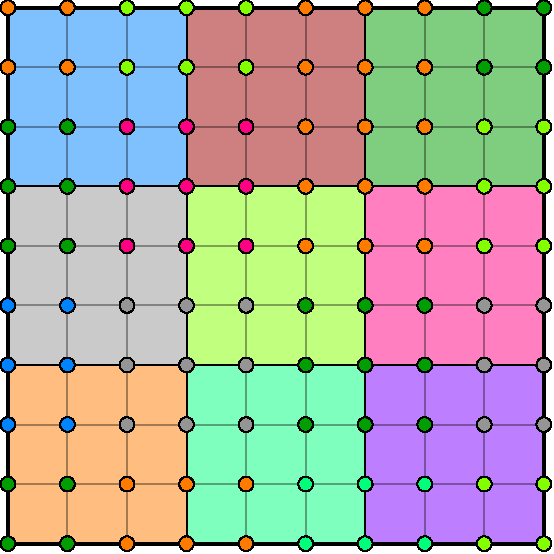
\includegraphics[width=0.9\linewidth]{figs/square_cart_struct_node_part}}
  \end{subfigure}
  \hfill
  \begin{subfigure}[t]{0.3\textwidth}
    \centerline{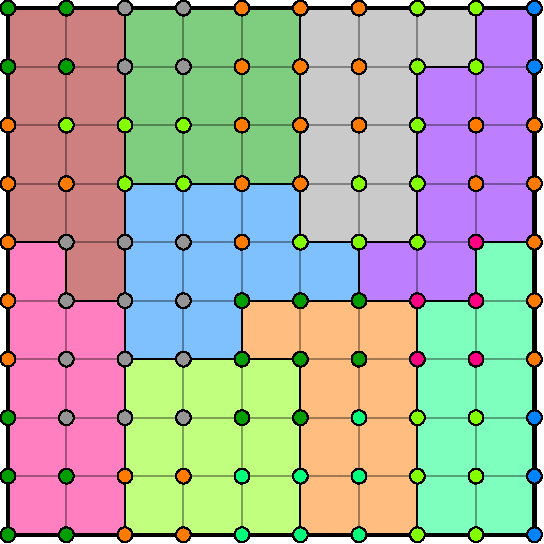
\includegraphics[width=0.9\linewidth]{figs/square_cart_metis_node_part}}
  \end{subfigure}
  \hfill
  \begin{subfigure}[t]{0.3\textwidth}
    \centerline{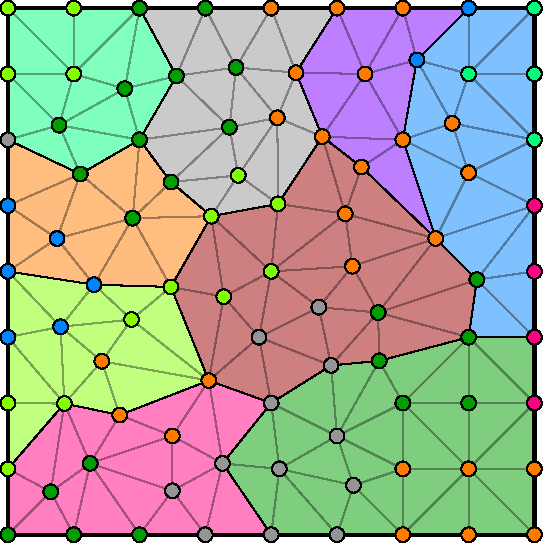
\includegraphics[width=0.9\linewidth]{figs/square_tria_metis_node_part}}
  \end{subfigure}
  \par\bigskip
  \begin{subfigure}[t]{0.3\textwidth}
    \centerline{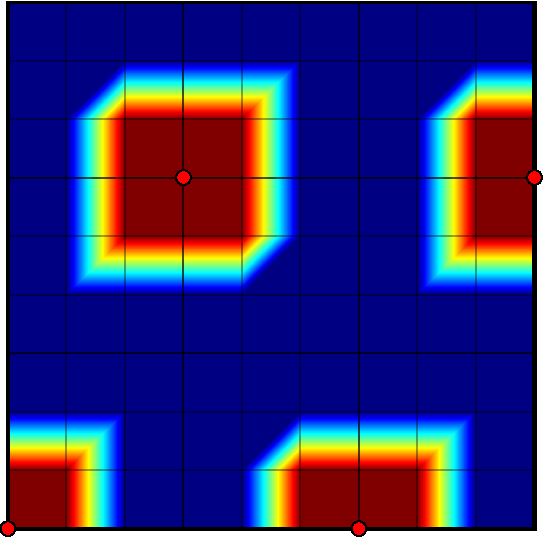
\includegraphics[width=0.9\linewidth]{figs/square_cart_struct_node_init}}
  \end{subfigure}
  \hfill
  \begin{subfigure}[t]{0.3\textwidth}
    \centerline{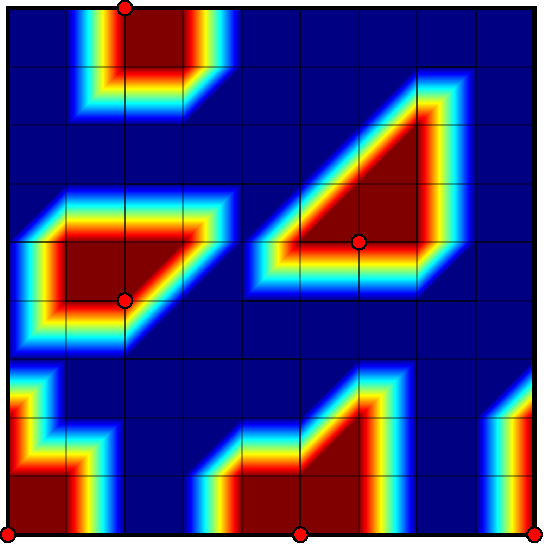
\includegraphics[width=0.9\linewidth]{figs/square_cart_metis_node_init}}
  \end{subfigure}
  \hfill
  \begin{subfigure}[t]{0.3\textwidth}
    \centerline{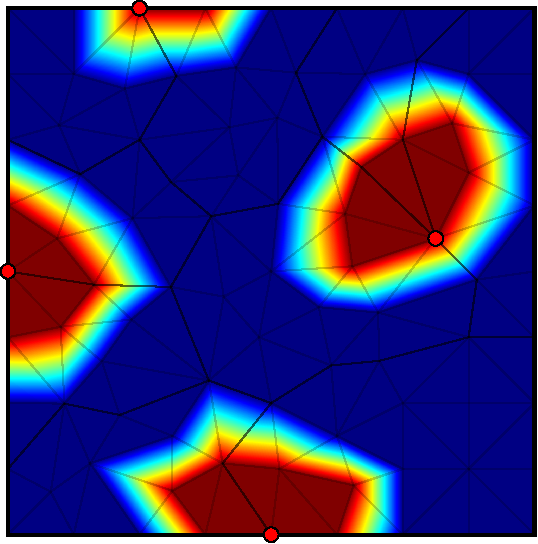
\includegraphics[width=0.9\linewidth]{figs/square_tria_metis_node_init}}
  \end{subfigure}
  \par\bigskip
  \begin{subfigure}[t]{0.3\textwidth}
    \centerline{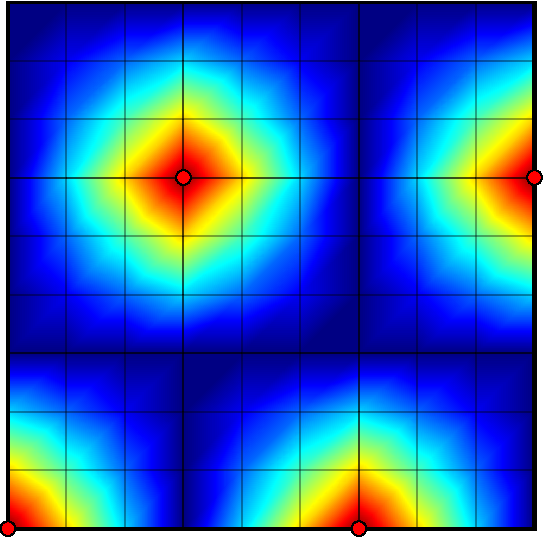
\includegraphics[width=0.9\linewidth]{figs/square_cart_struct_node_conv}}
  \end{subfigure}
  \hfill
  \begin{subfigure}[t]{0.3\textwidth}
    \centerline{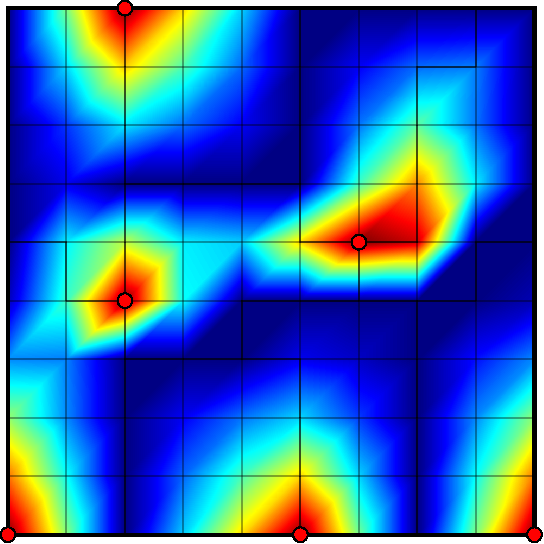
\includegraphics[width=0.9\linewidth]{figs/square_cart_metis_node_conv}}
  \end{subfigure}
  \hfill
  \begin{subfigure}[t]{0.3\textwidth}
    \centerline{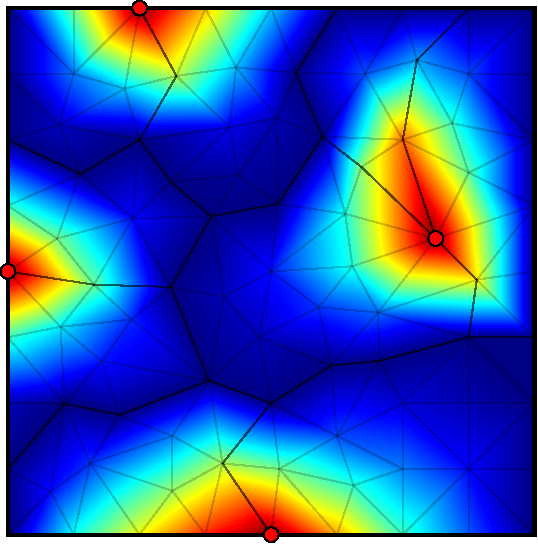
\includegraphics[width=0.9\linewidth]{figs/square_tria_metis_node_conv}}
  \end{subfigure}
  \caption[Nodal partitions and basis function examples]{\label{fig:square_node_basis} Examples of nodal partitions (top row) and select corresponding initial (middle row) and converged (bottom row) basis functions with support boundaries shown in (\Colorcircle{yellow}) for different types of grids/coarsening: fully structured (left), graph-coarsened structured (middle) and fully unstructured (right).   In all cases material is homogeneous and no boundary conditions are applied to the matrix used to compute basis functions.}
\end{figure}

\begin{figure}[htbp]
  \begin{subfigure}[t]{0.3\textwidth}
    \centerline{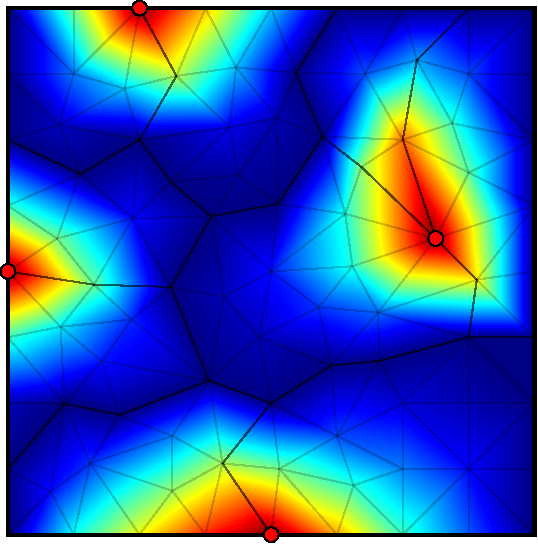
\includegraphics[width=0.9\linewidth]{figs/square_tria_metis_node_conv}}
  \end{subfigure}
  \hfill
  \begin{subfigure}[t]{0.3\textwidth}
    \centerline{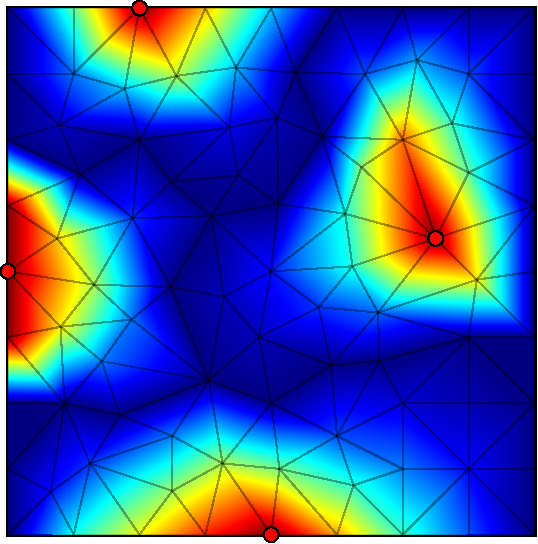
\includegraphics[width=0.9\linewidth]{figs/square_tria_metis_node_conv_bc_nonsymm}}
  \end{subfigure}
  \hfill
  \begin{subfigure}[t]{0.3\textwidth}
    \centerline{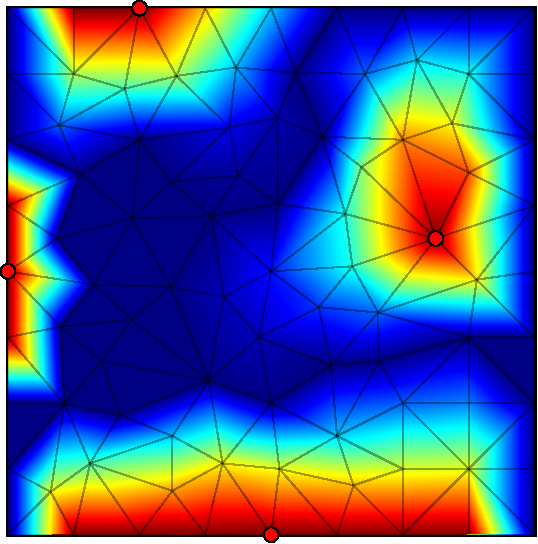
\includegraphics[width=0.9\linewidth]{figs/square_tria_metis_node_conv_bc_symm}}
  \end{subfigure}
  \caption[Nodal basis function with boundary condition effects]{\label{fig:square_node_bc} Examples of converged $x$-displacement basis functions without (left) and with non-symmetric (middle) and symmetric (right) application of Dirichlet boundary conditions to the system matrix.   Only normal displacement is prescribed on each side of the domain while tangential direction is unconstrained.}
\end{figure}

Finally, it's worth pointing out how the mechanisms of basis construction described earlier transfer to coarser grids when the number of levels exceeds two.   \autoref{fig:square_node_ml} shows an example of a fine mesh that is coarsened twice to obtain first and second level coarse grids.   Due to the flexibility of grid representation, the same algorithms are applied at each level to locate coarse nodes, build support regions, boundaries and compute tentative interpolation.   Note that second level prolongation operator is numerically defined on a discrete set of points corresponding to first level coarse nodes, but from a mathematical standpoint it can be viewed as belonging to the same function space as the finite element solution (piecewise linear functions on fine-scale elements), since the sequence of underlying finer-scale basis (or shape) functions can be used to compute its value anywhere in the domain.    Therefore rightmost image of \autoref{fig:square_node_ml} plots it on the fine grid by interpolating it using first-level prolongation operator.    In general, interpolation operator $P^{(k)}$ at any level $k$ can be interpreted on the fine grid via 
\begin{align}
    P^{(k),f} = \prod\limits_{i=1}^{k}P^{(i)} = P^{(1)}P^{(2)} \ldots P^{(k)}
\end{align}

\begin{figure}[htbp]
  \begin{subfigure}[t]{0.3\textwidth}
    \centerline{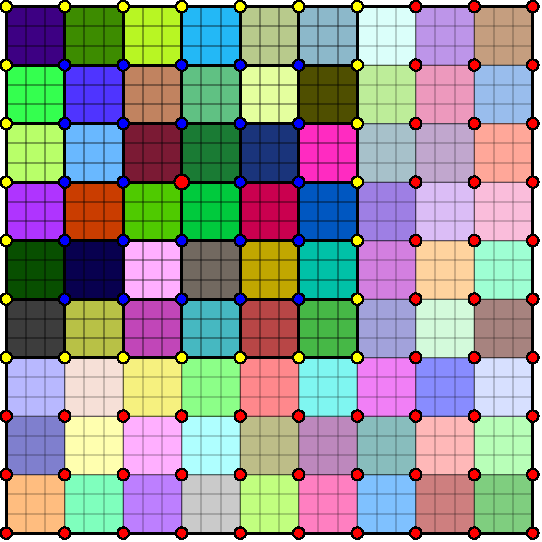
\includegraphics[width=0.9\linewidth]{figs/square_cart_struct_node_ml_lvl1_grid}}
  \end{subfigure}
  \hfill
  \begin{subfigure}[t]{0.3\textwidth}
    \centerline{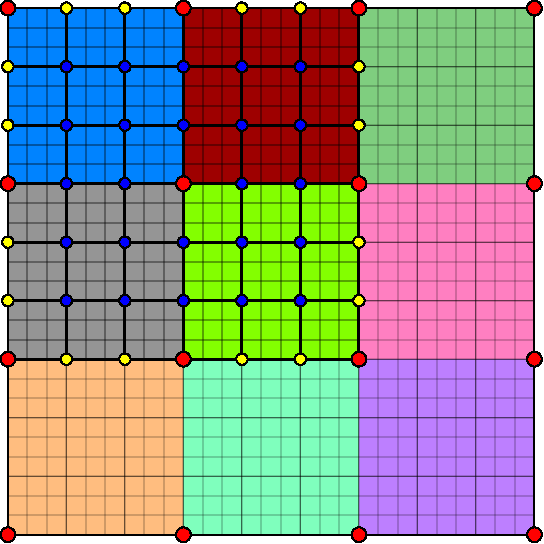
\includegraphics[width=0.9\linewidth]{figs/square_cart_struct_node_ml_lvl2_grid}}
  \end{subfigure}
  \hfill
  \begin{subfigure}[t]{0.3\textwidth}
    \centerline{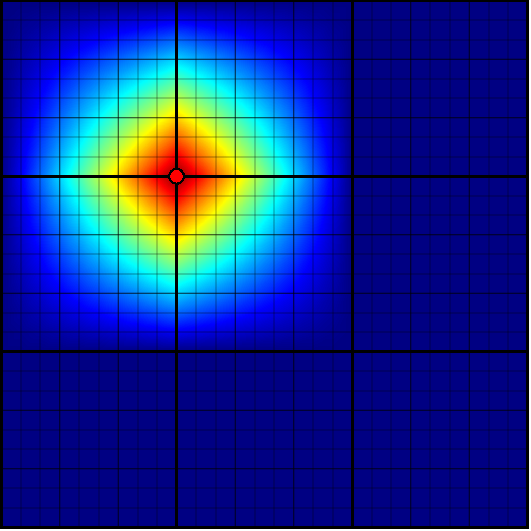
\includegraphics[width=0.9\linewidth]{figs/square_cart_struct_node_ml_lvl2_basis}}
  \end{subfigure}
  \par\bigskip
  \begin{subfigure}[t]{0.3\textwidth}
    \centerline{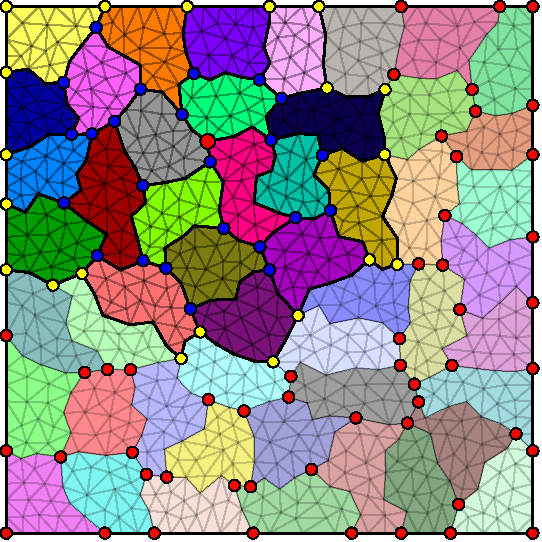
\includegraphics[width=0.9\linewidth]{figs/square_tria_metis_node_ml_lvl1_grid}}
  \end{subfigure}
  \hfill
  \begin{subfigure}[t]{0.3\textwidth}
    \centerline{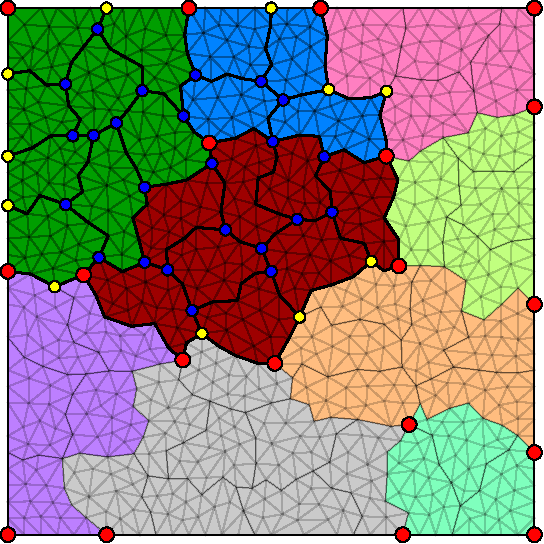
\includegraphics[width=0.9\linewidth]{figs/square_tria_metis_node_ml_lvl2_grid}}
  \end{subfigure}
  \hfill
  \begin{subfigure}[t]{0.3\textwidth}
    \centerline{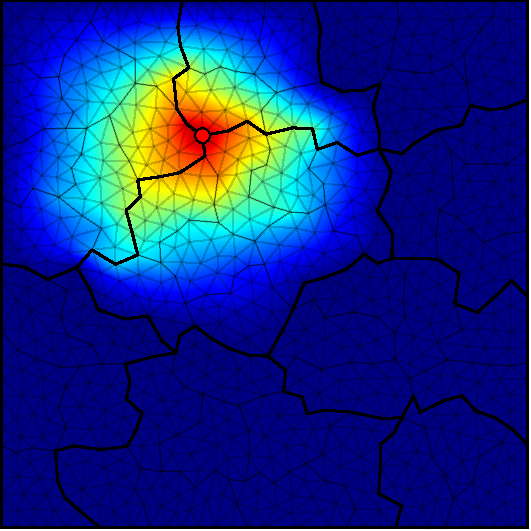
\includegraphics[width=0.9\linewidth]{figs/square_tria_metis_node_ml_lvl2_basis}}
  \end{subfigure}
  \caption[Higher level coarse grids and basis functions]{\label{fig:square_node_ml} Nodal basis construction on higher coarse grid levels: first level coarse grid (left); second level coarse grid (middle) obtained by partitioning first-level coarse cells; second level coarse basis function (right).   Coarse nodes are shown in (\Colorcircle{red}), support and boundary nodes for the basis function in (\Colorcircle{blue}) and (\Colorcircle{yellow}), respectively. Node marker size indicates the coarse grid level.}
\end{figure}

\subsection{Cell-Centered Basis Functions}
\label{subsec:msrsb_cell_basis}

In cell-centered multiscale methods (both MsFV and original MsRSB) the support of a basis function is defined to be a region surrounding the coarse cell center and extending to, but not including, centers of neighboring coarse cells (those sharing at least one coarse interface or node with the current one).   In MsFV this is formalized through the concept of a dual grid, with edges and faces typically formed by cells intersected by lines or planes connecting neighbor cells.   This dual grid (or, equivalently, the ''wirebasket'' labeling of unknowns) is explicitly constructed using Cartesian indexing logic on structured grids or more geometric algorithms on more complex topologies.   In MsRSB the authors used geometric triangulation of (a convex hull of) a local set of points of interest (coarse cell centers and interface midpoints) as a quick way to query and select cells lying within support and then form boundaries by extending another layer of cells, thus forming an approximate dual grid.   In both approaches, it is desirable for the interface cell layers between different support regions to match and be as thin as possible (for either accuracy or computational efficiency reasons).   The method proposed herein shares this goal, but attempts to construct support regions with perfectly matching single-cell layer boundaries using topological information only.

The task of constructing dual interfaces in a two-dimensional grid has a fairly simple solution that involves computing shortest paths between each pair of neighboring coarse cell centers in the fine-scale cell adjacency graph $\mathcal{G}_C^h$.   This can be achieved quickly using Dijkstra's algorithm applied to a subgraph limited only to cells belonging to the coarse cells of interest.   The solution, however, does not generalize well to three dimensions, where the problem of computing a minimal surface connecting a set of graph nodes is significantly more challenging.   Therefore a different approach is desired, and it comes from exploiting the duality between nodes and cells in a mesh.   Indeed, it is well known that the dual of a mesh $\mathcal{T}$ is a Voronoi mesh $\mathcal{T}^D$ of the same dimension in which vertices correspond to cell centroids of $\mathcal{T}$ and cells are formed by shortest-distance volumes around vertices of $\mathcal{T}$.   A similar definition can be extended to coarse grids formed by cell partitions --- in that case, the dual coarse volume corresponding to a coarse node is formed by a set of fine nodes topologically closest to that node, the dual coarse node is represented by a fine cell adjacent to a (locally) maximal number of dual coarse volumes, and the rest of fine cells adjacent to more than one dual coarse volume form the interfaces, analogous to fine nodes in a primal coarse mesh.   In \autoref{subsec:msrsb_nodal_basis} a simple procedure was presented for forming a nodal partitioning induced by a primal cell partitioning, which produces clusters of nodes corresponding exactly to topologically closest node agglomerates (Voronoi-like node partitions).   In \autoref{subsec:msrsb_coarsening_algorithm} a graph-based algorithm for selecting coarse nodes given cell-node adjacency was presented, which can also be used to analyze the dual node partitions.   Therefore all components for building an approximate graph-based dual coarse grid are available.   

The algorithm for constructing the dual coarse grid proceeds as follows:
\begin{enumerate}
    \item Let $\vec{z}_N^h \in [1,N_N^H]^{N_N^h}$ be the node partitioning vector obtained as a result of performing node clustering procedure from \autoref{subsec:msrsb_nodal_basis}.
    \item Each fine-scale cell $i \in [1,N_E^h]$ is assigned a key $K_i$ consisting of the indices of adjacent node partitions:
    \begin{align}
        K_i = \Set{ k \in [1,N_N^H] \mid \exists j \in [1,N_N^h]: (i,i) \in \mathcal{G}_E^h \:\text{and}\: [\vec{z}_N^h]_j = k }
    \end{align}
    \item Cells sharing the same key are grouped together into a feature into $N_F$ cell features, represented by cell grouping vector $\vec{z}_F^h \in [1,N_F]^{N_E^h}$, with $N_F$ the total number of features.
    \item A cell feature adjacency graph $\mathcal{G}_F$ is formed by connecting a pair of features if any of their cells share a common node in $\mathcal{G}_E^h$:
    \begin{align}
        \mathcal{G}_F = \set{(f_i,f_j) \bigm| \exists n \in [1,N_N^h], e_k, e_l \in [1,N_E^h]: (e_k,n), (e_l,n) \in \mathcal{G}_E^h, [\vec{z}_F^h]_k = i, [\vec{z}_F^h]_l = j}
    \end{align}
    \item Any feature $j$ whose key is fully subsumed by one of its neighbors ($K_j \subset K_i, (i,j) \in \mathcal{G}_F$ is removed from the candidate set.
    \item All remaining features are marked as ''vertex'' cells of the dual grid.   In case there are multiple cells in any feature, any one may be selected.
\end{enumerate}
Note that steps 2--6 are similar to the coarse node selection algorithm of \autoref{subsec:msrsb_coarsening_algorithm}.   In fact, they can be carried out by the same implementation while only swapping the inputs: replacing input graph $\mathcal{G}_{E}^h$ with its transpose $(\mathcal{G}_{E}^h)^T$ (transposing its adjacency matrix) and cell partitioning vector $\vec{z}_E^h$ with node partitioning vector $\vec{z}_N^h$ obtained in step 1.   The resulting dual coarse grids, along with the nodal partitions that produce them, are shown in the top row of \autoref{fig:square_cell_dual}, with coarse dual vertex cells highlighted in red color.   Marked in yellow are cells that are shared by more than one coarse dual cell --- they make up the support boundary sets $B_j$ as well as the global boundary set $B$.   All the other fine-scale cells belong to interior of one the dual coarse cells.

One can observe that the above algorithm results in more coarse dual vertex cells than there are primal coarse cells, except for a purely Cartesian grid.   Indeed, in a completely unstructured setting it is impossible to guarantee that topologically grown nodal agglomerates meet in exactly one location in each coarse cell (which would be the ideal outcome), even when good heuristics are used to guide the growth of nodal agglomerates.   Thus the proposed algorithm constructs a dual grid that is not an exact (optimal) dual of the primal coarse grid.    The rest of the method can proceed without issues, however there will be more coarse cell-centered degrees-of-freedom, and some of them will be clustered closely together.   This can lead to an increase in computational cost (in both construction and use) and memory footprint of the multiscale operator without a corresponding increase in interpolation quality.   Moreover, the coarse-scale system will no longer be consistent with the fine-scale cell partitioning, which presents a conceptual problem when applying the algorithm recursively.    This is addressed by simple post-processing of the dual coarse grid, in which a single dual vertex cell is selected out of every group belonging to the same coarse cell, and a union of adjacent nodal partitions is taken to compute the support.

Examples of post-processed dual grids are shown in bottom row of \autoref{fig:square_cell_dual}.   Obviously, no difference is observed for the completely structured case, since the initial dual grid induced by nodal partitioning perfectly matches what would be produced by a structured (Cartesian index-based) approach.   In other cases, post-processing effectively forces a single vertex cell per primal coarse partition, while preserving the dual edges induced by the nodal partition.   These edges no longer connect two dual coarse vertices directly, but form a more complex network with multiple forks and joints.   Nevertheless, there is still a single edge passing through each primal coarse cell interface.    Similar (albeit rather difficult to visualize effectively) result is obtained in three dimensions, with a network of dual surfaces approximating dual interfaces.

\begin{figure}[htbp]
  \begin{subfigure}[t]{0.3\textwidth}
    \centerline{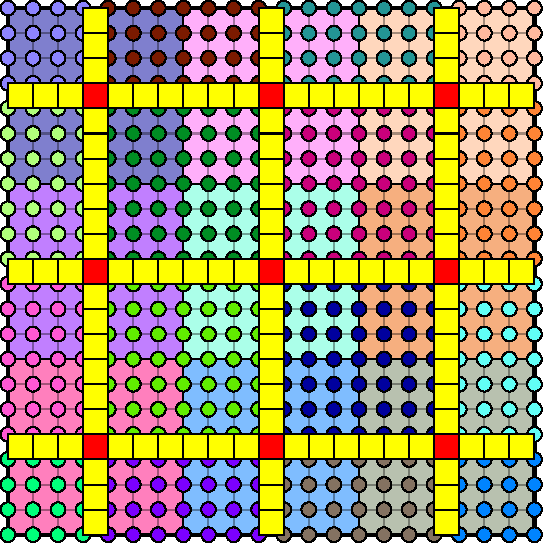
\includegraphics[width=0.9\linewidth]{figs/square_cart_struct_cell_dual_nomerge}}
  \end{subfigure}
  \hfill
  \begin{subfigure}[t]{0.3\textwidth}
    \centerline{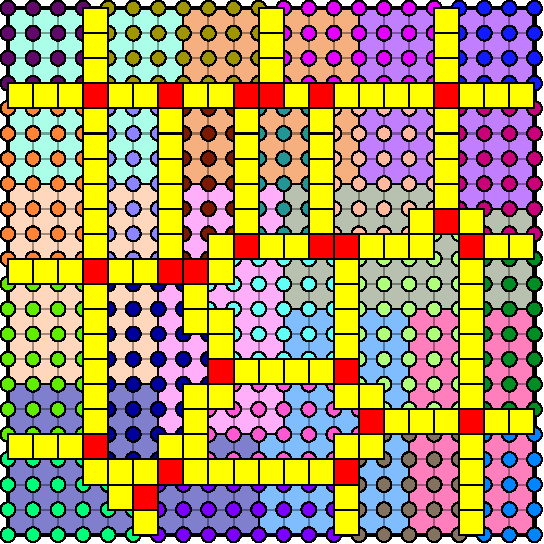
\includegraphics[width=0.9\linewidth]{figs/square_cart_metis_cell_dual_nomerge}}
  \end{subfigure}
  \hfill
  \begin{subfigure}[t]{0.3\textwidth}
    \centerline{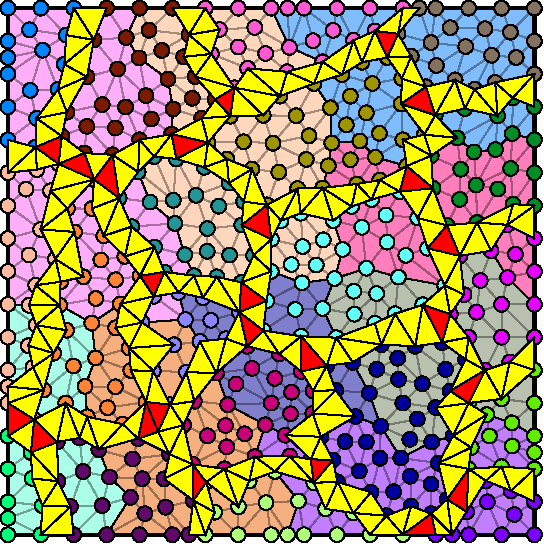
\includegraphics[width=0.9\linewidth]{figs/square_tria_metis_cell_dual_nomerge}}
  \end{subfigure}
  \par\bigskip
  \begin{subfigure}[t]{0.3\textwidth}
    \centerline{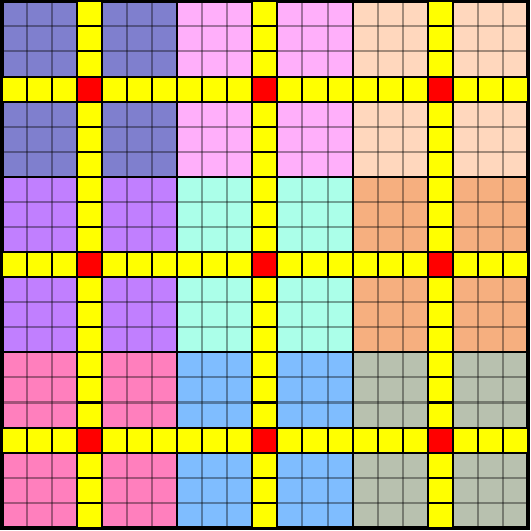
\includegraphics[width=0.9\linewidth]{figs/square_cart_struct_cell_dual}}
  \end{subfigure}
  \hfill
  \begin{subfigure}[t]{0.3\textwidth}
    \centerline{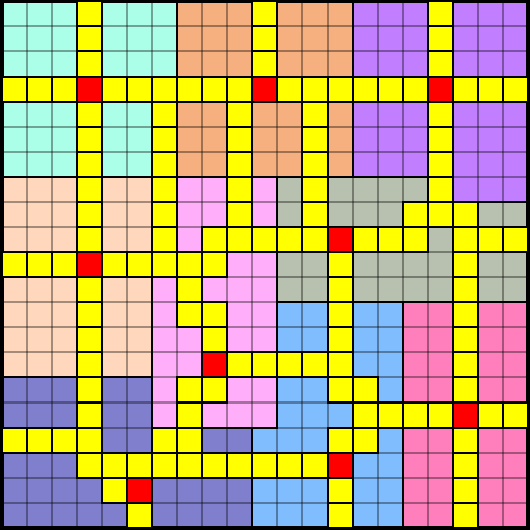
\includegraphics[width=0.9\linewidth]{figs/square_cart_metis_cell_dual}}
  \end{subfigure}
  \hfill
  \begin{subfigure}[t]{0.3\textwidth}
    \centerline{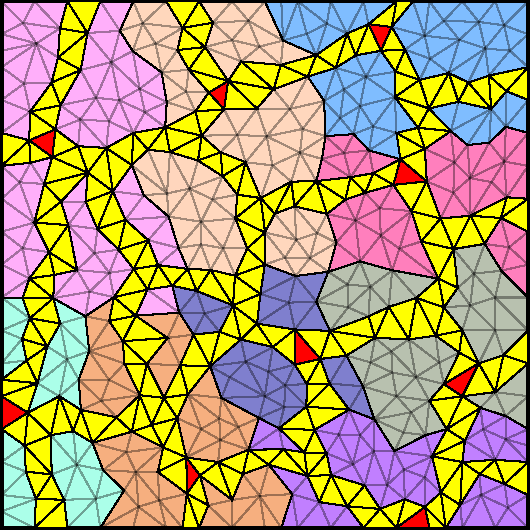
\includegraphics[width=0.9\linewidth]{figs/square_tria_metis_cell_dual}}
  \end{subfigure}
  \caption[Dual grid for cell-centered basis functions]{\label{fig:square_cell_dual} Examples of nodal partitions and induced dual coarse grids (top row) and post-processed dual coarse grids (bottom row) with support boundaries shown in (\Colorsquare{yellow}) and coarse dual vertex cells in (\Colorsquare{red}) for different types of grids/coarsening: fully structured (left), graph-coarsened structured (middle) and fully unstructured (right).   The coarsening ratios are intentionally chosen to be small to simplify presentation.}
\end{figure}

The support region for a coarse basis function associated with one of the dual coarse vertex cells is constructed in almost the same way as in the case of nodal basis functions: $I_j$ is the set of fine-scale cells adjacent exclusively to nodes in nodal partitions neighboring the vertex cell.   The same procedure may be used to build support regions $I_j$ and boundary sets $B_j$.   One major difference is that we don't need to introduce additional virtual subdomains representing global domain boundaries, which was a specific treatment required by nodal basis.   The initial basis functions take a much simpler form compared to nodal basis: following original MsRSB work, we can simply use an indicator function that assigns 1 for each fine cell within the primal coarse cell, and 0 outside.  \autoref{fig:square_cell_basis} demonstrates examples of support regions resulting from various kinds of post-processed dual grids, as well as initial and converged basis functions.   An important consequence of the post-processing procedure implemented is that fine cells that fall on dual edges connecting the merged vertex cells always keep the basis function value of 1, i.e. are always interpolated to the value of the vertex cell.   This occurs because they happen to be on the support boundary for every other basis functions, and tends to somewhat decrease quality of the interpolation operator.   The lengths of these constant interpolation streaks vary with grid and partition quality, but they tend to make up a few percent of the coarse cell volume.   In an approximate multiscale solver this would lead to systematic errors in the interpolated solution, but in the context of a preconditioner it can be acceptable without loss of scalability due to action of the second stage that can resolve these localized errors.

\begin{figure}[htbp]
  \begin{subfigure}[t]{0.3\textwidth}
    \centerline{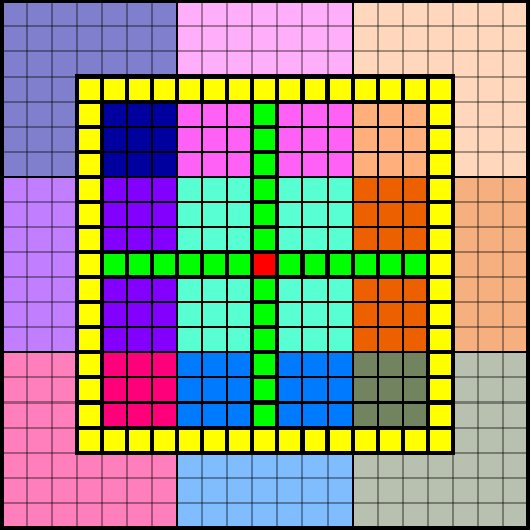
\includegraphics[width=0.9\linewidth]{figs/square_cart_struct_cell_supp}}
  \end{subfigure}
  \hfill
  \begin{subfigure}[t]{0.3\textwidth}
    \centerline{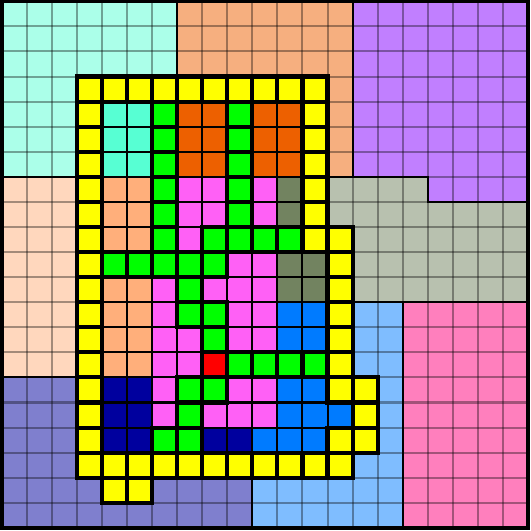
\includegraphics[width=0.9\linewidth]{figs/square_cart_metis_cell_supp}}
  \end{subfigure}
  \hfill
  \begin{subfigure}[t]{0.3\textwidth}
    \centerline{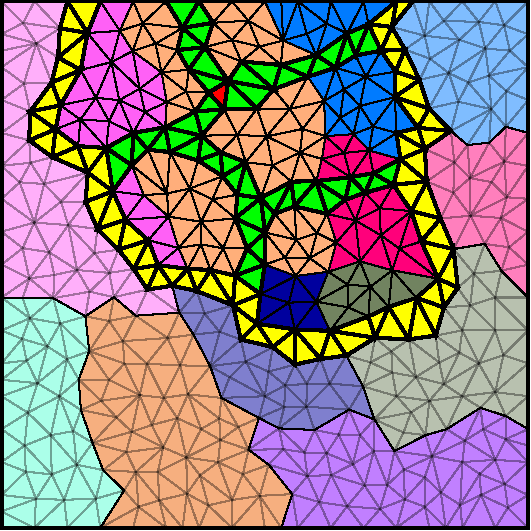
\includegraphics[width=0.9\linewidth]{figs/square_tria_metis_cell_supp}}
  \end{subfigure}
  \par\bigskip
  \begin{subfigure}[t]{0.3\textwidth}
    \centerline{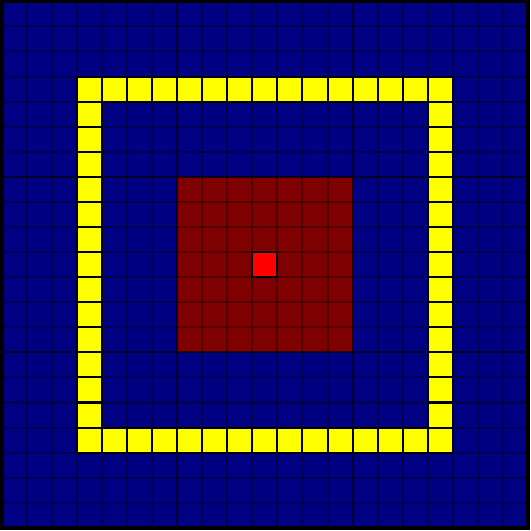
\includegraphics[width=0.9\linewidth]{figs/square_cart_struct_cell_init}}
  \end{subfigure}
  \hfill
  \begin{subfigure}[t]{0.3\textwidth}
    \centerline{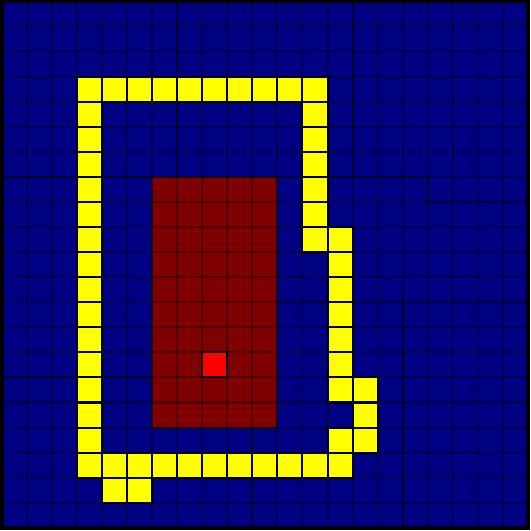
\includegraphics[width=0.9\linewidth]{figs/square_cart_metis_cell_init}}
  \end{subfigure}
  \hfill
  \begin{subfigure}[t]{0.3\textwidth}
    \centerline{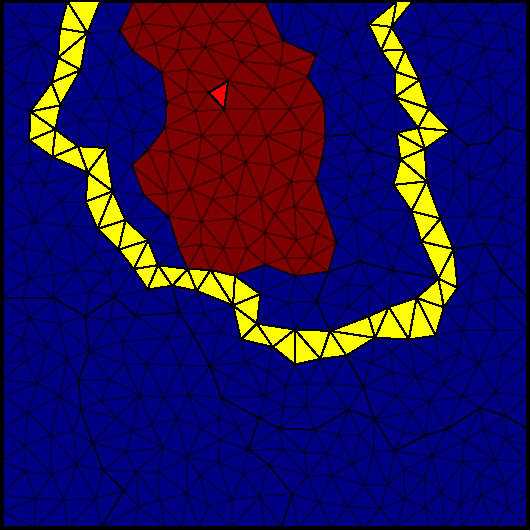
\includegraphics[width=0.9\linewidth]{figs/square_tria_metis_cell_init}}
  \end{subfigure}
  \par\bigskip
  \begin{subfigure}[t]{0.3\textwidth}
    \centerline{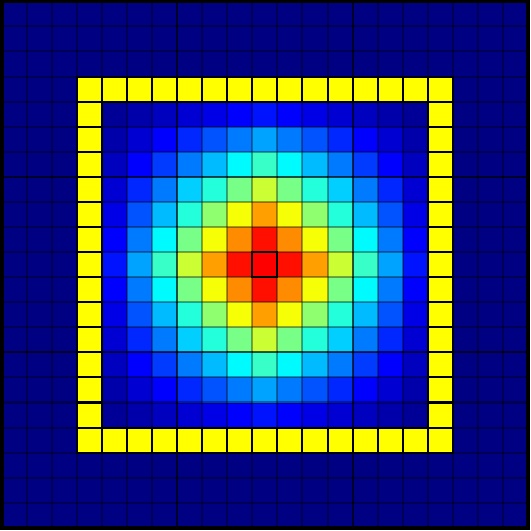
\includegraphics[width=0.9\linewidth]{figs/square_cart_struct_cell_conv}}
  \end{subfigure}
  \hfill
  \begin{subfigure}[t]{0.3\textwidth}
    \centerline{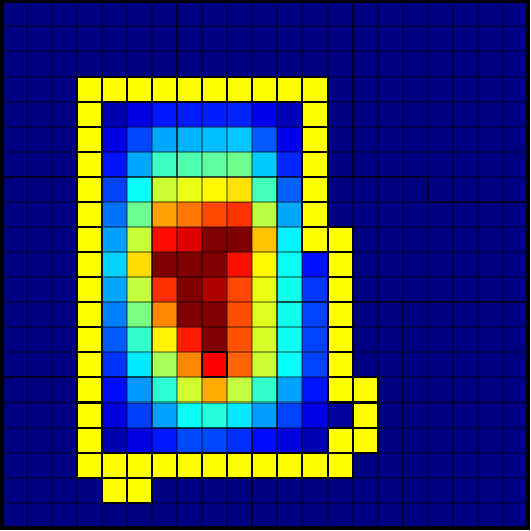
\includegraphics[width=0.9\linewidth]{figs/square_cart_metis_cell_conv}}
  \end{subfigure}
  \hfill
  \begin{subfigure}[t]{0.3\textwidth}
    \centerline{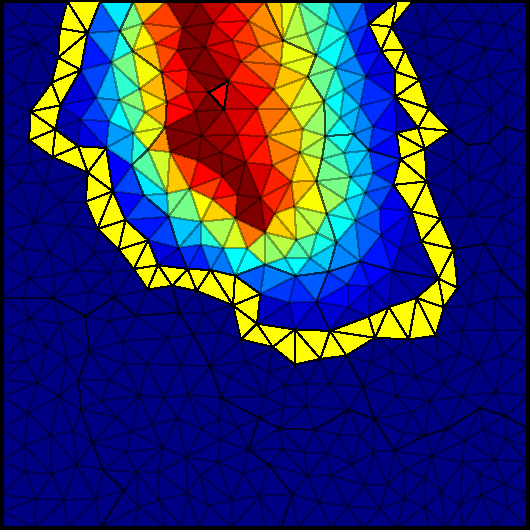
\includegraphics[width=0.9\linewidth]{figs/square_tria_metis_cell_conv}}
  \end{subfigure}
  \caption[Cell-centered support and basis function examples]{\label{fig:square_cell_basis} Examples of cell-centered support regions (top row) and initial (middle row) and converged (bottom row) basis functions with outer support boundaries shown in (\Colorsquare{yellow}), interior support boundaries in (\Colorsquare{green}) and coarse dual vertex cells in (\Colorsquare{red}) for different types of grids/coarsening: fully structured (left), graph-coarsened structured (middle) and fully unstructured (right).}
\end{figure}

We remark that MsRSB method does not necessarily require matching dual interfaces, and allows the definition of support regions to be arbitrary; in particular support regions corresponding to basis functions centered on non-neighboring coarse cells may in general overlap.   For example, \cite{Klemetsdal2020} used a ''simple growth'' algorithm for constructing support regions (extending initial shape of the primal aggregate by a given number of cell layers), suggesting also that a similar approach is used in MsRSB implementation of a commercial simulation software package.   While simpler to implement, this approach requires additional care.   If an insufficient number of layers are used, parts of the domain may be interpolated by a single basis function, leading to patches of constant interpolation similar to the aforementioned issue of our method but potentially larger in size.   If too many layers are used, sparsity pattern of the coarse system may grow very quickly due to overlapping supports of non-neighbor basis functions.   This can be remedied by using sparsification strategies based on ad-hoc dropping rules and tolerances (also known as non-Galerkin coarse grids in multigrid literature), but such approaches are not always effective and may lead to degradation of convergence.   On the other hand, support regions that are defined by a globally matching (approximate) dual grid are guaranteed by construction to not increase stencil sizes (beyond an initial increase from TPFA to MPFA-style stencil at the first level).   Indeed, when computing $A^H = RA^hP$ triple product, $A^hP$ has a sparsity pattern that extends a single cell layer beyond that of $P$, meaning that a basis function (a column of $P$) now has nonzero values on its support boundary, but aside from immediate neighbors, no other basis function in rows of $R$ has nonzero values on those boundary cells, and thus no extra ''non-neighbor'' connections are introduced.

Similar to nodal case, cell-centered basis functions on coarser grid levels of a multilevel scheme are defined recursively, using finer-level basis to interpolate and interpret them on the fine scale (using piecewise constant shape functions on each element), as shown in \autoref{fig:square_cell_ml} for a three-level scheme.   In the idealized case of Cartesian grid with structured coarsening and homogeneous material, the second coarse level basis functions are identical to ones that would be constructed in a two-level scheme utilizing the coarsest grid directly; in most other cases however grid effects of the first coarse level can be observed.   One caveat of a multilevel cell-centered method is that coarse degree-of-freedom collocation points tend to get further away from the boundary as the number of levels increases, leaving a widening layer with constant interpolation at domain boundaries, which negatively affects convergence.   One must therefore avoid over-coarsening (using too many levels), or additional post-processing of the dual grid must be employed to shift or place additional coarse cell centers closer to domain boundaries.

\begin{figure}[htbp]
  \begin{subfigure}[t]{0.3\textwidth}
    \centerline{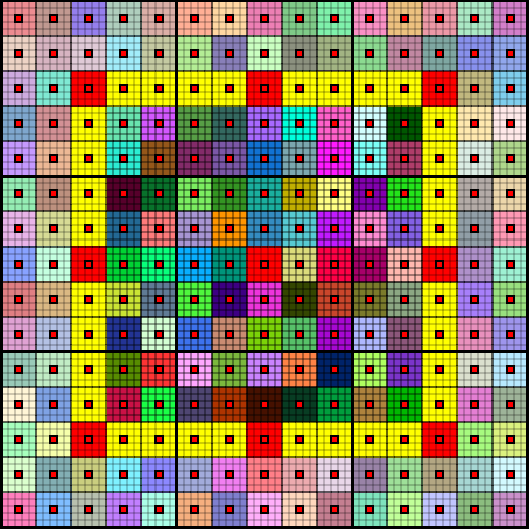
\includegraphics[width=0.9\linewidth]{figs/square_cart_struct_cell_ml_lvl1_grid}}
  \end{subfigure}
  \hfill
  \begin{subfigure}[t]{0.3\textwidth}
    \centerline{\includegraphics[width=0.9\linewidth]{figs/square_cart_struct_cell_ml_lvl2_grid}}
  \end{subfigure}
  \hfill
  \begin{subfigure}[t]{0.3\textwidth}
    \centerline{\includegraphics[width=0.9\linewidth]{figs/square_cart_struct_cell_ml_lvl2_basis}}
  \end{subfigure}
  \par\bigskip
  \begin{subfigure}[t]{0.3\textwidth}
    \centerline{\includegraphics[width=0.9\linewidth]{figs/square_tria_metis_cell_ml_lvl1_grid}}
  \end{subfigure}
  \hfill
  \begin{subfigure}[t]{0.3\textwidth}
    \centerline{\includegraphics[width=0.9\linewidth]{figs/square_tria_metis_cell_ml_lvl2_grid}}
  \end{subfigure}
  \hfill
  \begin{subfigure}[t]{0.3\textwidth}
    \centerline{\includegraphics[width=0.9\linewidth]{figs/square_tria_metis_cell_ml_lvl2_basis}}
  \end{subfigure}
  \caption[Higher level coarse grids and  cell-centered basis functions]{\label{fig:square_cell_ml} Cell-centered basis construction on higher coarse grid levels: first level coarse grid (left); second level coarse grid (middle) obtained by partitioning first-level coarse cells; second level coarse basis function (right).   Coarse cell centers are shown in (\Colorsquare{red}), boundary cells for the basis function in (\Colorsquare{yellow}), respectively.}
\end{figure}

%\subsection{Error and Spectral Analysis}
%\label{subsec:msrsb_analysis}

%\subsection{Alternative Coarsening Strategy}
%\label{subsec:msrsb_cell_basis_alt}

% ===================== SECTION =====================
\section{Preconditioning for Coupled Systems}
\label{sec:coupled_precond}

We now address preconditioning for coupled single-phase poroelastic systems discretized fully implicitly using first-order finite element method for displacements and cell-centered finite volume method for pressure.   Linearized discrete problem of this type takes the form:
\begin{align}
    \begin{bmatrix}
        A_{uu}^h & A_{up}^h \\
        A_{pu}^h & A_{pp}^h
    \end{bmatrix}
    \begin{bmatrix}
        \vec{u}^h \\
        \vec{p}^h
    \end{bmatrix} =
    \begin{bmatrix}
        \vec{f}_u^h \\
        \vec{f}_p^h
    \end{bmatrix}
    \label{eq:coupled_poroelastic_linear_system}
\end{align}
where off-diagonal blocks $A_{up}^h$ and $A_{pu}^h$ capture the effect of the Biot poroelastic coupling.   This is a coupled system of two elliptic (or elliptic-like) equations which exhibits interactions at a range of spatial scales, therefore it is suited to be solved by a multilevel scheme.   In this section we devise a preconditioning scheme that addresses the coupled problem.   The poroelastic preconditioner follows the general two-stage multiscale solver template described in \autoref{subsec:related_work_msfv}, with a global coarse grid correction operator and a local smoother combined multiplicatively at every level.   Both stages are described in detail below.    We remark two differences from much of the published multiscale work:
\begin{itemize}
    \item The smoother in this method is applied, by default, both before and after coarse grid step, in line with most multigrid methods (but as an option, pre- or post-smoothing can be disabled).
    \item The method is multilevel by default, that is, coarse level solve consist of another application of multiscale preconditioner.   The level hierarchy can be truncated either by a hard limit on number of levels, or by setting a lower limit on number of degrees of freedom that should be coarsened further.
\end{itemize}

\subsection{Coupled Interpolation and Coarse Problem}
\label{subsec:coupled_interpolation}

In order to define the global (multiscale) operator $\mathcal{M}_G$ \eqref{eq:coupled_poroelastic_linear_system}, a prolongation must be defined that simultaneously interpolates displacement and pressure values at the fine-scale (herein we assume a Galerkin method with $R = P^T$).   In order to be compatible with the coupled system matrix, the operator must also possess the block form
\begin{align}
    P = 
    \begin{bmatrix}
        P_{uu} & P_{up} \\
        P_{pu} & P_{pp}
    \end{bmatrix}
    \label{eq:coupled_prolongation_general}
\end{align}

Given a coarse mesh, two possibilities to define such an operator using MsRSB method arise naturally:
\begin{itemize}
    \item Initialize diagonal blocks of \eqref{eq:coupled_prolongation_general} using same indicator functions as in their respective single-physics methods functions.   Then perform smoothing iteration \eqref{eq:msrsb_update}-\eqref{eq:msrsb_check} on the coupled matrix until convergence on the full set of basis functions.
    \item Perform smoothing iteration separately for displacement and pressure basis functions, using only $A_{uu}^h$ and $A_{pp}^h$ blocks, respectively.   Define a block-diagonal prolongation operator
    \begin{align}
        P = 
    \begin{bmatrix}
    P_{uu} &        \\
           & P_{pp}
    \end{bmatrix}
    \label{eq:coupled_prolongation}
    \end{align}
\end{itemize}

The first approach results in a set of coupled basis functions that incorporate local (fine-scale) interaction effects between displacement and pressure.   However, the smoothing iteration is not guaranteed to converge in general for the coupled system, or may take a very long time to do so.   Moreover, the software implementation of this approach is somewhat more cumbersome, requiring non-trivial modifications of otherwise black-box implementations of the flow and mechanics preconditioners.   In particular, pressure (cell-centered) support for displacement basis functions and displacement (nodal) support regions for pressure basis functions must be defined, which determine the sparsity pattern of $P_{pu}$ and $P_{up}$ blocks, respectively.   Therefore we opt for the second approach, where the basis functions for each coarse degree-of-freedom only interpolate their corresponding fine-scale counterparts.   This roughly corresponds to drained conditions for mechanics (no contributions to stress from fluid pressure) and fixed-strain conditions for flow (flow in undeformed porous medium), although an option to construct a fixed-stress Schur complement approximation for $A_{uu}^h$ is also available, as explained in \autoref{subsec:coupled_smoothing}.

In addition to a more straightforward implementation, an important advantage of this choice is the lack of requirement on the coarse grids for displacement and pressure to match.   Indeed, each of the $P_{uu}$ and $P_{pp}$ block's computation does not affect the other, which allows for completely independent choice of coarse grids.   For example, separate coarsening ratios may be used for the two problems, reflecting the difference in the scales of variation in the underlying material properties.   Although not considered in present work, even the case where fine-scale discretization is carried out on two different grids can be supported (which of course requires the user to provide adjacency information for both grids).   Even though the total number of levels in the preconditioner must be the same for both sub-problems in order for the coupled coarse problem to be well-defined, each can independently choose when to truncate the coarsening and effectively preserve the coarsest grid resolution through the remaining levels.   Thus, the choice of block-diagonal interpolation provides a great deal of flexibility with respect to tuning parameter space.   Note that this choice is similar to the ''monolithic AMG'' approach of \cite{Gee2011,Verdugo2016} which has been successfully applied in fluid-structure interaction and other multiphysics problems with strong elliptic components.

We remark that the coarse-scale system remains coupled even with this choice of prolongation:
\begin{align}
    \begin{bmatrix}
		R_{uu} &       \\
		       & R_{pp}
	\end{bmatrix}
	\begin{bmatrix}
		A_{uu}^h & A_{up}^h \\
		A_{pu}^h & A_{pp}^h
	\end{bmatrix}
	\begin{bmatrix}
	    P_{uu} &       \\
		       & P_{pp}
	\end{bmatrix} =
	\begin{bmatrix}
	    R_{uu} A_{uu}^h P_{uu} & R_{uu} A_{up}^h P_{pp} \\
	    R_{pp} A_{pu}^h P_{uu} & R_{pp} A_{pp}^h P_{pp}
	\end{bmatrix} =
	\begin{bmatrix}
		A_{uu}^H & A_{up}^H \\
		A_{pu}^H & A_{pp}^H
	\end{bmatrix}
	\label{eq:coupled_poroelastic_coarse_system}
\end{align}
with all blocks nonzero.   Therefore the coupling between mechanics and flow is taken into account at the coarse scale, and remaining fine-scale errors resulting from interpolation deficiency can be effectively accounted for be the coupled smoother, described in the following subsection.   Coarsest-scale system with matrix \eqref{eq:coupled_poroelastic_coarse_system} can be solved with a direct solver, or any other solver suitable for a coupled system of this type.

\subsection{Block-Triangular Smoothing via Fixed-Stress Approximation}
\label{subsec:coupled_smoothing}

The local smoother for the coupled system can be designed following the existing body of work on preconditioners for coupled poroelasticity \cite{White2011,White2015,Castelletto2015,Castelletto2019}.   Namely, block Gaussian elimination on system matrix $J$ of \eqref{eq:coupled_poroelastic_linear_system} yields block upper-triangular form:
\begin{align}
    \begin{bmatrix}
        A_{uu}^h & A_{up}^h \\
                 & S_{pp}^h
    \end{bmatrix}
    \label{eq:coupled_poroelastic_schur_system}
\end{align}
with
\begin{align}
    S_{pp}^h &= A_{pp}^h - A_{pu}^h (A_{uu}^h)^{-1} A_{up}^h \label{eq:coupled_poroelastic_schur_complement}
\end{align}
where $S_{pp}^h$ is the Schur complement of $A_{uu}^h$.   The matrix $(A_{uu}^h)^{-1}$, and consequently $(S_{pp}^h)^{-1}$, generally is dense and expensive to compute directly, therefore an inexpensive sparsity-preserving approximation $\tilde{S}_{pp}^h$ is desirable.   Such an approximation can be obtained based on one of several approaches:
\begin{itemize}
    \item Physics-based construction as proposed in \cite{White2015}:
    \begin{align}
        \tilde{S}_{pp}^h = A_{pp}^h + \frac{b^2}{K_{dr}}M_p
    \end{align}
    with $b$ the Biot coefficient, $K_{dr}$ the drained bulk modulus of the solid and $M_p$ the pressure space mass matrix (which, for the case of finite-volume flow discretization, turns into a diagonal matrix of cell volumes).
    \item Element-by-element inverse approximation proposed in \cite{Castelletto2016}:
    \begin{align}
        \tilde{S}_{pp}^h = \sum\limits_{i=1}^{N_c^h} [A_{pu}^h]_{i,:} [A_{uu}^h]_{(i)}^{-1} [A_{up}^h]_{:,i} \vec{e}_i \vec{e}_i^T
    \end{align}
    with $[A_{uu}^h]_{(i)}$ the sub-matrix of $A_{uu}^h$ corresponding to nodes of element $i$, $[A_{pu}^h]_{i,:}$ the $i$-th row of $A_{pu}^h$ and $[A_{up}^h]_{:,i}$ the $i$-th column of $A_{up}^h$.
    \item Diagonal approximation of the leading block:
    \begin{align}
        \tilde{S}_{pp}^h = A_{pp}^h - A_{pu}^h (D_{uu}^h)^{-1} A_{up}^h
    \end{align}
    with $D_{uu}$ the diagonal of $A_{uu}^h$.   Note that the sparsity pattern of the subtracted term which represents cell connections through a shared vertex may be wider than that of $A_{pp}^h$ when TPFA scheme is used; in that case, the extra terms are dropped or lumped into diagonal in order to avoid modifying the sparsity pattern (typically an expensive operation).
    \item Probing technique used in \cite{Klevtsov2016}:
    \begin{align}
        \tilde{S}_{pp}^h = A_{pp}^h - \Diag(A_{pu}^h \mathcal{M}_u^{-1} A_{up}^h \vec{e})
    \end{align}
    where $\mathcal{M}_u^{-1}$ is some preconditioner or solver capable of cheaply approximating the action of $(A_{uu}^h)^{-1}$ on a vector (possibly a single multiscale or multigrid cycle), and
    \begin{align}
        \vec{e} = \sum\limits_{i=1}^{N_c^h}\vec{e}_i
    \end{align}
    is the probing vector with every element equal to 1.   The idea behind probing with this particular vector is that the diagonal approximation constructed this way preserves row sums of the exact Schur complement and thus amounts to diagonal lumping.   Computing $\tilde{S}_{pp}^h$ this way involves two matrix-vector multiplications and one solve with an approximate mechanics solver
\end{itemize}
In this work, diagonal and probing-based approximations are used, owing to their fully algebraic character and simplicity of implementation.   It's worth mentioning that in the context of block smoothing, the construction of accurate Schur complement approximation is less important, compared to full-fledged fine-scale block preconditioners, so $\mathcal{M}_u^{-1}$ may be chosen to be very cheap.   Moreover, as $A_{uu}^h$, $A_{up}^h$ and $A_{pu}^h$ are constant for a linear elastic solid model under small strain assumption and fixed displacement boundary conditions (a typical modeling scenario), $\tilde{S}_{pp}^h$ can only be computed once and reused for the rest of the simulation run.

Assuming efficient local smoothers are available separately for $A_{uu}^h$ ($\mathcal{M}_{L,u}^{-1}$) and $\tilde{S}_{pp}^h$ ($\mathcal{M}_{L,p}^{-1}$), the system \eqref{eq:coupled_poroelastic_schur_system} can now be preconditioned with a block upper-triangular operator
\begin{align}
    \mathcal{M}_L^{-1} =
    \begin{bmatrix}
        \mathcal{M}_{L,u} & A_{up}^h          \\
                          & \mathcal{M}_{L,p}
    \end{bmatrix}^{-1}
    =
    \begin{bmatrix}
        \mathcal{M}_{L,u}^{-1} & -\mathcal{M}_{L,u}^{-1} A_{up}^h \mathcal{M}_{L,p}^{-1} \\
                               &  \mathcal{M}_{L,p}^{-1}
    \end{bmatrix}
\end{align}

The above form, applied to a vector $\vec{v}$, amounts to
\begin{align}
    \vec{z} = \mathcal{M}_L^{-1}\vec{v} = 
    \begin{bmatrix}
        \mathcal{M}_{L,u}^{-1} & -\mathcal{M}_{L,u}^{-1} A_{up}^h \mathcal{M}_{L,p}^{-1} \\
                               &  \mathcal{M}_{L,p}^{-1}
    \end{bmatrix}
    \begin{bmatrix}
        \vec{v}_u \\
        \vec{v}_p
    \end{bmatrix}
    =
    \begin{bmatrix}
        \mathcal{M}_{L,u}^{-1} \left(\vec{v}_u - A_{up}^h (\mathcal{M}_{L,p}^{-1} \vec{v}_p)\right) \\
        \mathcal{M}_{L,p}^{-1} \vec{v}_p
    \end{bmatrix}
\end{align}
which in turn is equivalent to a multiplicative combination of $\mathcal{M}_{L,p}^{-1}$ and $\mathcal{M}_{L,u}^{-1}$, applied in two steps:
\begin{enumerate}
    \item Compute $\vec{z}_p = \mathcal{M}_{L,p}^{-1} \vec{v}_p$
    \item Compute $\vec{z}_u = \mathcal{M}_{L,u}^{-1}(\vec{v}_u - A_{up}^h \vec{z}_p)$
\end{enumerate}

The specific choice of Schur approximation above corresponds to the so-called fixed-stress operator, widely used as an operator splitting and iterative solution technique and shown to be unconditionally stable \cite{Kim2011b} and highly effective.   Other choices are available for the shape of the preconditioning operator, for example block diagonal or lower-triangular (employed in \cite{White2019}).   In the context of a preconditioned iterative method, all of them are approximately equivalent, since the outer iteration provides exchange of information in both directions via residual updates (with possible error orthogonalization steps in between).   Alternative approaches include constructing a Schur complement $S_{uu}^h$ of $A_{pp}^h$, or simply ignoring the Schur complement and using block diagonal of system matrix \eqref{eq:coupled_poroelastic_linear_system} for preconditioning.   These approaches are less effective as shown by \cite{White2015}, and ultimately the construction of the smoother is a relatively small fraction of the overall setup cost.

\subsection{Multiscale Preconditioner for Multiphase Poromechanics}
\label{subsec:coupled_multiphase}

The methods developed in present work focus primarily on efficient elliptic solvers for single-phase poroelasticity.   However, fully implicit modeling of coupled multiphase flow and mechanics is of practical interest for many applications, such as geological storage of CO\textsubscript{2}, unconventional oil and gas reservoirs and more.   Here we briefly present a preconditioning framework for multiphase poromechanics with two options to incorporate multiscale methods developed previously in this work.   It combines the ideas of the widely used and proven Constrained Pressure Residual preconditioner for coupled flow and transport \cite{Wallis1983} and fixed-stress preconditioning discussed earlier.   For simplicity, in the remainder of this subsection superscript $h$ will be omitted and the matrices will refer to the fine scale, unless noted otherwise.

Specifically, a fully implicit discretization of the multiphase poromechanics system \eqref{eq:momentum_balance_mp}-\eqref{eq:mass_balance_mp} results in a matrix that, permuted into the block form, can be written as
\begin{align}
    A = 
    \begin{bmatrix}
        A_{uu} & A_{up} & A_{us} \\
        A_{pu} & A_{pp} & A_{ps} \\
        A_{su} & A_{sp} & A_{ss}
    \end{bmatrix}
    \label{eq:multiphase_poromechanics_block_form}
\end{align}
where $u$ denotes displacement and momentum balance equations; subscript $p$ denotes pressure unknown and total mass balance equation; subscript $s$ represents transport variables (typically phase saturations $S^\alpha$, component mole/mass fractions $y_i^\alpha$ or combinations thereof) when used as block column index and mass conservation equations of individual components (except one) when used as block row index.   One can observe that block $A_{us}$ describes the effect of transport unknowns on momentum balance.   Phase saturations influence momentum balance through mixture density terms affecting gravity forces and possibly, depending on the modeling approach, through average pore pressure included in total stress.   Both of these effect are relatively weak unless capillary pressure difference between phases is high compared to reference phase pressure or sharp contrast is present in phase densities.   For the rest of this section we will make the approximation $A_{us} \approx 0$ for preconditioning purposes.

The first approach follows \cite{White2019} and consists of a two-level reduction scheme in which mechanical and flow/transport problems are separated first, using view of the system partitioned as
\begin{align}
    A = 
    \begin{bmatrix}
        A_{uu} & A_{uf} \\
        A_{fu} & A_{ff}
    \end{bmatrix}
\end{align}
with subscript $f$ indicating flow/transport unknowns and equations.   The outer preconditioner is based on approximate inverse of the upper triangular form of $A$
\begin{align}
    \begin{bmatrix}
        A_{uu} & A_{uf} \\
               & S_{ff}
    \end{bmatrix}
\end{align}
with probing-based Schur complement approximation
\begin{align}
    S_{ff} &= A_{ff} - A_{fu}A_{uu}^{-1}A_{uf} \\
    \tilde{S}_{ff} &= A_{ff} - \Diag(A_{fu}\mathcal{M}_u^{-1}A_{uf}\vec{e})
\end{align}
and reads
\begin{align}
    \mathcal{M}_I^{-1} =
    \begin{bmatrix}
        \mathcal{M}_{uu} & A_{uf}          \\
                         & \mathcal{M}_{f}
    \end{bmatrix}^{-1}
    =
    \begin{bmatrix}
        \mathcal{M}_{u}^{-1} & -\mathcal{M}_{u}^{-1} A_{uf}^h \mathcal{M}_{f}^{-1} \\
                             &  \mathcal{M}_{f}^{-1}
    \end{bmatrix}
\end{align}
Here $\mathcal{M}_f^{-1} \approx \tilde{S}_{ff}^{-1}$ represents the standard two-stage CPR operator:
\begin{align}
    \mathcal{M}_f^{-1} = \mathcal{M}_{f,G}^{-1} + \mathcal{M}_{f,L}^{-1}\left(I - \tilde{S}_{ff}\mathcal{M}_{f,G}^{-1}\right)
\end{align}
with a local smoother $\mathcal{M}_{f,L}^{-1}$ applied to the overall flow/transport system ordered cell-wise, and the global operator $\mathcal{M}_{f,G}^{-1}$ consisting of (True-IMPES or Quasi-IMPES) restriction to the pressure system combined with a pressure solver $\mathcal{M}_p^{-1}$.   The key ingredients --- efficient elliptic solvers $\mathcal{M}_u^{-1}$ and $\mathcal{M}_p^{-1}$ --- consist of an application of the multilevel multiscale methods described in this chapter (typically just a single up/down cycle).   Thus, coupling between pressure and displacement is resolved only at the fine scale, which may require a few more iterations overall, but each of the two multiscale cycles is separate from the other and can choose its depth independently.   The fact that the setup of $\mathcal{M}_p^{-1}$ is based on the CPR pressure system (which incorporates the influence of transport and thus changes between Newton iterations and time steps) highlights one of the strengths of MsRSB approach - the ability to incrementally update basis functions by making only a few smoothing iterations.

The second approach extends the ideas presented in \cite{Klevtsov2016} in which hyperbolic transport unknowns are decoupled from the (approximately) elliptic displacement-pressure system.
Namely, the outer preconditioner takes a standard two-stage local-global form:
\begin{align}
    \mathcal{M}_{II}^{-1} = \mathcal{M}_{II,G}^{-1} + \mathcal{M}_{II,L}^{-1}\left(I - A \mathcal{M}_{II,G}^{-1}\right)
\end{align}
in which the local smoother $\mathcal{M}_{II,L}^{-1}$ is a block smoother similar in design to the one described in \autoref{subsec:coupled_smoothing} but with a block variant of the smoother applied to cell-wise ordered flow/transport block $A_{ff}$ instead of $A_{pp}$.   The global operator builds on a CPR-type reduction of the form:
\begin{align}
    A_{ee} =
    \begin{bmatrix}
        A_{uu} - A_{us} D_{ss}^{-1} A_{su} & A_{up} - A_{us} D_{ss}^{-1} A_{sp} \\
        A_{pu} - D_{ps} D_{ss}^{-1} A_{sp} & A_{pp} - D_{ps} D_{ss}^{-1} A_{sp}
    \end{bmatrix}
    =
    \begin{bmatrix}
        A_{uu}         & A_{up} \\
        \tilde{A}_{pu} & \tilde{A}_{pp}
    \end{bmatrix}
    = R^{cpr} A P^{cpr}
\end{align}
with subscript $e$ denoting the elliptic part of the problem, $D_{ss}$ and $D_{ps}$ are block diagonalizations of the corresponding blocks of $A$ (based on True-IMPES or Quasi-IMPES approach), and we have taken into account the approximation $A_{us} \approx 0$.   In the above,
\begin{align}
    R^{cpr} = 
    \begin{bmatrix}
                             & I &   \\
        - D_{ps} D_{ss}^{-1} &   & I
    \end{bmatrix}
    \quad\quad\quad
    P^{cpr} =
    \begin{bmatrix}
          &   \\
        I &   \\
          & I 
    \end{bmatrix}
\end{align}
Finally, the coupled multiscale preconditioner is applied to the elliptic system with matrix $A_{ee}$:
\begin{align}
    \mathcal{M}_{II,G}^{-1} = P^{cpr} \mathcal{M}_{MS,poro}^{-1} R^{cpr}
\end{align}
As shown previously, this preserves and accounts for mechanics-flow coupling at every level.   Thus, this scheme might be preferred in cases in which this coupling is particularly strong throughout the domain.

\subsection{Treatment of Wells}
\label{subsec:coupled_wells}

Finally, handling of wells by the multiscale method must be discussed.   Numerical well models manifest as additional flux terms in perforated cells and/or additional equations representing mass balance in the well, as described in \autoref{?}.   In most examples presented later in this chapter, boundary conditions for the flow problem are represented by single perforation wells.   Such wells do not need a dedicated control equation, and their effect on the system is expressed either through a right-hand side contribution (for rate-controlled wells) or both right-hand side and diagonal matrix contribution (for pressure-controlled wells).   For multi-perforation wells a separate control equation is formed, and for even more complex multi-segmented well models multiple mass balance equations and associated degrees-of-freedom introduced, leading to the following partition of the system matrix:
\begin{align}
    A^h =
    \begin{bmatrix}
        A_{pp}^h & A_{pw}^h \\
        A_{wp}^h & A_{ww}^h
    \end{bmatrix}
\end{align}
with $A_{pp}^h$ representing the matrix of the flow problem.   Following \cite{Moyner2016}, present method preserves all well equations and unknowns at every level of coarsening, as expressed by the following definition of $P$:
\begin{align}
    P =
    \begin{bmatrix}
        P_{pp} &        \\
               & I_{ww} \\
    \end{bmatrix}
\end{align}
with $I_{ww}$ an identity matrix of the size equal to the number of well equations.   This leads to a coarse system computed via
\begin{align}
    \begin{bmatrix}
		R_{pp} &       \\
		       & I_{ww}
	\end{bmatrix}
	\begin{bmatrix}
		A_{pp}^h & A_{pw}^h \\
		A_{wp}^h & A_{ww}^h
	\end{bmatrix}
	\begin{bmatrix}
	    P_{pp} &       \\
		       & I_{ww}
	\end{bmatrix} =
	\begin{bmatrix}
	    R_{pp} A_{pp}^h P_{pp}   & R_{pp} A_{pw}^h \\
	    A_{wp}^h P_{pp} & A_{ww}^h
	\end{bmatrix} =
	\begin{bmatrix}
		A_{pp}^H & A_{pw}^H \\
		A_{wp}^H & A_{ww}^H
	\end{bmatrix}
\end{align}
with $A_{ww}^H = A_{ww}^h$ and the terms in $A_{pw}^H$ and $A_{wp}^H$ representing effective coarse-level well transmissibilities obtained by a weighted sum of fine-scale transmissibilities of current well's perforations within each dual coarse cell.   The well equations are eventually resolved by the coarsest-level solver and well unknowns keep their values through the prolongation process, while smoothers deal with remaining local errors.   We also remark that presence of wells bears no effect on the pressure basis functions: no additional basis functions for wells are introduced, and diagonal contributions of well transmissibilities to the flow matrix are effectively neglected during the smoothing procedure (by enforcing the zero row sum condition necessary to guarantee partition of unity preservation).

% ===================== SECTION =====================
\section{Numerical Examples}
\label{sec:msrsb_examples}

In this section we evaluate the proposed multilevel multiscale method from a purely algorithmic viewpoint.   We investigate its robustness and algorithmic scalability as a preconditioner, i.e. its ability to ensure convergence of an iterative linear solver for a range of problem sizes and physical parameters.   Most of the numerical experiments described below are carried out using a prototype implementation, and thus absolute metrics such as CPU time are not reported.   Such measurements are provided in \autoref{ch:parallel_multiscale} where we investigate parallel scalability using an optimized implementation.

\subsection{Test Cases Setup}

\subsection{Algorithmic Scalability}

\subsection{Heterogeneity and Anisotropy}

\subsection{Effect of Coarsening Parameters}

% ===================== SECTION =====================
\section{Summary}
\label{sec:msrsb_summary}

\chapter{High-Performance Multiphysics Simulation Framework}
\chaptermark{Multiphysics Simulation Framework}
\label{ch:geosx_framework}

% ===================== SECTION =====================
\section{Introduction}
\label{sec:geosx_intro}

This chapter presents the overall design and several key components of a new multiphysics modeling framework targeting state-of-the-art and future massively parallel architectures, including upcoming exascale systems, called GEOSX \cite{geosx}, which is a collaborative effort between research groups from several institutions and companies \cite{geosx-website}.   We detail a few important contributions to the framework, including the development of compositional multiphase flow solver and linear algebra solver components, as well as describing the data structures and interfaces that form the foundation for the implementation of parallel multiscale preconditioner.

\subsection{Motivation and Design Goals}
\label{subsec:geosx_motivation}

Sustainable energy transition must rely heavily on a variety of subsurface energy systems, including  geological carbon storage (GCS) reservoirs, unconventional natural gas resources and geothermal systems.   A thorough understanding of the dynamic behavior of these systems is needed to predict and optimize their performance and ensure safety of operation.   Their behavior is driven by several tightly coupled physical processes, most notably porous media flow, transport, geomechanics and geochemistry, over a large range of spatiotemporal scales.   For example, when modeling injection into GCS deep saline reservoirs, accurate prediction of pressure buildup and associated mechanical deformation and stresses helps ensure the integrity of the cap rock and manage the risks of fault activation, CO\textsubscript{2} leakage and induced seismicity, while detailed modeling of fluid-rock interaction across and chemical reactions across scales improves our understanding of the interplay between CO\textsubscript{2} trapping mechanisms and storage capacity of these systems.

Unfortunately, in many pre-existing simulation tools coupling between different physical processes has often either been ignored or added as an afterthought, leading to loosely coupled models that may lack sufficient prediction accuracy.   For example, many commercial workflows involve transfer of information between a flow and a geomechanical simulator at predefined time intervals.   Incorporating new physics and tight coupling into a well established simulation package is an extremely challenging task, since it often requires fundamental changes in software architecture which are difficult to achieve while maintaining robustness, user familiarity and a plethora of supported features.   On the other hand, research simulators have been successful at implementing the necessary changes and prototyping and developing advanced physics, numerical models and coupling schemes \cite{Rin2017,Garipov2018}, but may lack robustness and performance required for large-scale modeling efforts due to a different set of goals and priorities (e.g. focusing on cutting-edge research).

At the same time, a fast-paced change in high-performance computing landscape has brought about new architectures (most notably, GPUs) with thousands of processing cores and orders-of-magnitude gains in raw compute power but also sophisticated memory hierarchies and programming models that additional require effort to take advantage of.   Updating legacy code to efficiently take advantage of parallelism on these platforms is often impossible or infeasible due to the amount and complexity of infrastructural changes involved and the need to redesign or outright replace many algorithms with their scalable versions.   In addition, as the architectures quickly evolve, changes made for one platform may become obsolete and non-portable.   A code that is designed for fine-grained parallelism from the ground up and built on top of a solid and portable parallel programming model can avoid both of these problems.

GEOSX is conceived and developed fundamentally as a novel massively parallel framework for fully coupled multiphysics subsurface simulation, aimed at taking advantage of current and next-generation high-performance computing architectures.   A specific set of design goals are:
\begin{itemize}
    \item Flexibility: support unstructured geologic grids with complex fault and fracture networks and wells, while solving combinations of coupled flow, transport, geomechanics and heat transfer problems.
    \item Modularity: developers see a highly modularized framework of components that are easy to add, while users interact with a unified simulator.
    \item Performance: striving to achieve near-peak performance on current and future architectures.
    \item Portability: while optimal algorithms and data structures are architecture-dependent, those differences are hidden behind portability abstractions.
\end{itemize}

\subsection{Framework Overview}
\label{subsec:geosx_overview}

GEOSX is developed in C++14 language standard, with additional Python interfaces and supporting modules.   Language extensions for CUDA (Compute Unified Device Architecture) and HIP (Heterogeneous Interface for Portability), the two major programming models for GPUs, are used when building the code on those platforms.   The framework has a modular architecture, consisting or a number of loosely coupled components that address various aspects of simulator workflow, such as data management, file I/O, discretization methods, constitutive models, linear algebra.   \autoref{fig:geosx_components} shows a simplified structure of core components of GEOSX.   All of these components ultimately are employed to build a collection of physics solvers that address specific (combinations of) physical processes.   Each physics solver acts as a driver for advancing a given set of solution and state variables to the next time level and makes use of an independent set of computational kernels (implemented as separate objects that manage their own data and execution) that may be customized and reused across solvers to facilitate the development of new fully implicit coupled solvers.   Execution of GEOSX is event-driven, with solver time stepping, visualization outputs, checkpointing and other tasks all invoked and coordinated in a consistent manner based on both a prescribed schedule of events and dynamic time step selection.   Next, we describe several core components of the framework, highlighting some of our contributions and describing in detail the key ingredients that enable the development of scalable parallel solvers and preconditioners.

\begin{figure} [htbp]
  \centerline{\includegraphics[width=0.9\linewidth]{figs/geosx}}
  \caption[Diagram of major GEOSX components]{\label{fig:geosx_components} A simplified diagram of GEOSX components, grouped into several logical groups}
\end{figure}

\section{Key Components}
\label{sec:geosx_components}

\subsection{Performance Portability Layer}
\label{subsec:geosx_components_portability}

Given the requirement for the framework to be forward-compatible with upcoming computing systems, our approach to leveraging parallelism is built on top of libraries that abstract away the details of particular hardware platform and vendor-specific application programming interfaces (APIs) and compiler instructions.   Most architectures provide two primary types of explicit resources --- compute and memory --- and both need to be dealt with in a portable way.   GEOSX is built on top of two separate types of abstractions provided by separate but interoperating libraries.

\subsubsection{Execution Model Abstractions}

Compute resource, or execution model, refers to decomposition and assignment of work over a number of execution units (multi-core CPU thread pools or blocks of GPU threads).   Execution abstraction used in GEOSX are available through RAJA library \cite{Beckingsale2019,raja}.   Loops over index spaces are the primary way of expressing independent work, and the library provides a \texttt{forall} pattern for writing parallel loops (also referred to as \textit{kernels}) as well as patterns for more complex control flow such as nested loops which allow for more flexible work partitioning.   The pattern accepts an execution \textit{policy} parameter, which specifies on which compute resource and how the loop is to be parallelized, along with an index space to iterate over and the work to be executed for each element in that space (the kernel \texttt{body}).   Under the hood RAJA takes care of decomposing work, mapping it to execution units and invoking a platform-specific API to initiate the computation according to the chosen policy.   The kernel body may be any function object callable with a single index argument, and often takes the form of a \texttt{closure} object (the result of a \texttt{lambda} expression that defines an anonymous function object in-place), which can conveniently carry arbitrary context necessary for the computation (such as views into arrays of physical quantities).   

In addition to kernel launching, RAJA contains portable abstractions over frequently used architecture-specific features such as atomic operations and block-shared memory on GPU (which falls back to regular memory on CPU targets).   Portable reductions are available in the form of objects that can be copy-captured in kernels and accumulate the final reduced value upon kernel exit.   Finally, more complex patterns that require dedicated implementations on different platforms (such as scan and sort) are also provided by the library.   With this set of primitives, large classes of numerical algorithms may be easily expressed in a portable way, and adapting the code to a new platform usually takes the form of using a different execution policy (as long as the necessary backend is implemented in RAJA).

\begin{figure} [htbp]
  \begin{subfigure}[t]{0.45\textwidth}
    \centering
    \begin{minted}[fontsize=\small]{cpp}
for (int i = 0; i < N; ++i)
{
    // kernel body
    c[i] = a[i] + b[i];
}
    \end{minted}
    \caption{\label{fig:raja_example_cpp} A simple C++ loop.}
  \end{subfigure}
  \hfill
  \begin{subfigure}[t]{0.45\textwidth}
    \centering
    \begin{minted}[fontsize=\small]{cpp}
RAJA::forall<Policy>(0, N, [=] (int i)
{ 
    // kernel body
    c[i] = a[i] + b[i]; 
});
    \end{minted}
    \caption{\label{fig:raja_example_raja} An equivalent RAJA loop.}
\end{subfigure}
\caption[RAJA loop example]{\label{fig:raja_example} Example of a C++ loop converted into a parallel RAJA loop. \texttt{Policy} may alias one of \texttt{loop\_exec}, \texttt{omp\_exec}, \texttt{cuda\_exec<num\_threads>}, etc. depending on target architecture.   Arrays \texttt{a}, \texttt{b} and \texttt{c} must be accessible in the chosen execution space.}
\end{figure}

\subsubsection{Memory Space Abstractions}

The second portability concern of a framework like GEOSX is dealing with multiple memory spaces.   Memory systems in parallel architectures like GPUs are heterogeneous, meaning system memory is physically and logically partitioned and some partitions (referred to as memory spaces) may not be accessible by all execution units.   Therefore any data accessed by a kernel must be first allocated in and copied to an appropriate memory space, and copies should only be performed when necessary (e.g. when data has been most recently modified in a different space) to avoid incurring extra cost.   This need is addressed by CHAI library \cite{chai} which provides convenient interfaces for tracking and managing memory allocations across different spaces.   CHAI itself is using Umpire library \cite{Beckingsale2020} containing a collection of memory-space aware allocators that abstract platform-specific memory management APIs.   CHAI coordinates with RAJA to infer a memory space appropriate for the compute resource of currently executing kernel and intelligently decide whether data must be copied into that space.   All simulation data containers (described next) in GEOSX are built on top of CHAI-managed memory buffers.

\subsection{Data Structures}
\label{subsec:geosx_components_data}

\subsubsection{High-performance Containers}

To support the RAJA-based kernel execution model and facilitate multiple-memory space semantics, GEOSX provides a number of specialized containers that are used across the code to store all mesh and simulation data, including solution and state variables, mesh connectivity maps, discretization information, variable-length model parameters, and any other data that must be accessed by kernels.   These containers, along with various some additional utilities for writing portable code are grouped into a separate library \texttt{LvArray}.
\begin{itemize}
    \item \texttt{Array} is a fundamental multidimensional array type, parametrized on data type, number of dimensions and memory layout.   The number of dimensions is static (compile-time), but array extents along each dimensions are specified at runtime.   The memory layout is chosen statically based on optimal memory access pattern on the target architecture.   For example, a coalesced read occurs on GPU when the kernel iteration parameter is used to index a unit-stride dimension of the array (typically dimension 0, corresponding to cell or node index of the mesh).   This will be explained in more detailed in \autoref{sec:com}
    \item \texttt{SortedArray} is a 1D array maintaining a sorted order and uniqueness of its elements, which makes it a fast and space-efficient representation of a \texttt{set} abstract type (known as a \texttt{flatset}). Quick $O(\log_2 n)$ lookup is provided via binary search, while element insertion is $O(n)$.
    \item \texttt{ArrayOfArrays} is a container representing a \textit{ragged} 2D array, i.e. one with variable-size second dimension.   All data is stored in a contiguous memory allocation, with offsets to keep track of the start of each sub-array.   This memory layout reduces the number of allocations and the amount of indirection needed for access, and corresponds to a widely used CSR (Compressed Sparse Row) storage format for sparse matrices.   In GEOSX it is most frequently used to represent connectivity graphs in mesh data structures.   New elements can be appended to any sub-array in a parallel kernel as long as sufficient capacity has been pre-allocated for it.   Moreover, elements can be appended to the same sub-array by concurrent threads using atomic instructions to increment sub-array size, which facilitates the use of multi-threaded kernels to build mesh maps.
    \item \texttt{ArrayOfSets} is similar to \texttt{ArrayOfArrays}, but also maintains uniqueness and sorted order of elements in each sub-array, similar to \texttt{SortedArray}.
    \item \texttt{CRSMatrix} is built on top of \texttt{ArrayOfSets} but stores both columns and entries, sorted by column index, while also providing an API for atomic operations on entries with fixed sparsity pattern.   It is used by all physics solvers to efficiently perform parallel assembly of implicit system matrices before handing it off to a linear solver.
\end{itemize}
By default, each of the above containers is backed by one or several CHAI-based linear memory buffer.   Each type also comes with a corresponding \texttt{View} type, which is a short-lived, non-owning data accessor that cannot reallocate (e.g. by resizing) the underlying container, but can invoke a data migration to another memory space when copied into a kernel execution context.   View types also control the data migration patterns: a \texttt{constant} view allows only read access and thus does not mark the data ''dirty'' (i.e. potentially modified) in the space in which it is used.   When used correctly, view types provide a transparent copy-hiding mechanism that is widely relied upon in GEOSX to perform operations across memory spaces.   As will be explained in \autoref{ch:parallel_multiscale}, we have also built an efficient multilevel mesh data structure on top of these abstractions.

\subsubsection{Computational Grid}

GEOSX is designed from the ground up to support unstructured three-dimensional grids for modeling of a wide set of physics, and as such maintains an explicit representation and connectivity of all grid entities.   The grid is distributed across processes and each mesh object (cell, face, edge or node) is uniquely owned by one process, with possible ghosted representation on processes that own adjacent portions of the domain.   Each entity type is stored in an associated \texttt{Manager}, which provides useful services such as:
\begin{itemize}
    \item local-to-global (and inverse) mapping of object indices and ownership identification;
    \item management of associated data (registration, automatic sizing, (de-)serialization);
    \item synchronizing simulation data on ghosted objects (``halo exchanges``).
\end{itemize}
Each \texttt{Manager} also stores associated connectivity maps to other entities using the most efficient container, typically a 2D \texttt{Array} for fixed-size relations (e.g. each edge is connected to two nodes) or an \texttt{ArrayOfSets} for variable-sized ones (e.g. a node is connected to an arbitrary number of cells). 

Since GEOSX is designed for multiphysics simulations, the representation of elements has a more involved structure.   Elements of are grouped into \textit{regions} which allows for flexible mapping of physics and constitutive models to portions of the mesh (i.e. a solver may be assigned to a particular set of \textit{target} regions).   Each region type is specialized to a particular type of elements (e.g. 3D cells or 2D surfaces).   3D cell regions are further arranged into sub-regions by element shape (hexahedra, tetrahedra, etc.).    This allows us to use of memory-efficient data structures within each sub-region (2D arrays for face, edge and node maps).   Moreover, execution of finite-element kernels on GPU can be optimized, since for each sub-region key sizing parameters (number of nodes, quadrature points per element) can be made known at compile-time, through effective use of templates and static dispatching techniques, enabling loop unrolling and use of GPU registers.

\subsection{Constitutive Models}
\label{subsec:geosx_constitutive}

\subsubsection{Model Types}

GEOSX provides a large and extensible catalog of constitutive relations that describe various aspects of material (solid, fluid, etc.) behavior.   Models are grouped by their base type which defines model's interface in terms of input and output quantities.   Some of the commonly used model types (with examples of specific implementations):
\begin{itemize}
    \item solid deformation (elastic (transverse)isotropic/orthotropic, Drucker-Prager, Cam-Clay)
    \item single-phase fluid (slightly compressible)
    \item multiphase fluid (two-phase dead-oil, two- or three-phase black-oil, compositional EoS-based hydrocarbon, CO\textsubscript{2}-brine);
    \item porosity (constant, pressure-dependent, Biot)
    \item permeability (constant, Carman-Kozeny, parallel plates fracture)
    \item relative permeability (Brooks-Corey, Van Genuchten, Baker, table-based)
\end{itemize}
Each model implementation defines and can produce instances a companion \textit{compute} class (colloquially referred to as model's kernel \textit{wrapper}), that acts as a RAJA-friendly representation of the model that can be correctly copied into kernel execution contexts across memory spaces and used to perform computations.   In particular, a compute object contains inside of it memory-space aware \texttt{View}s into all relevant data, including model parameters and possible internal/history state (needed to implement hysteretic behavior).

\subsubsection{Constitutive Dispatch}

Since specific constitutive models are chosen by the user through input files, the framework needs a way to dispatch work to the right model during execution.   Traditional programming techniques for dealing with customizable behavior rely on dynamic dispatch, which usually takes the form of virtual functions or other similar types of indirect calls.   This works well when model computation across the entire grid points is \textit{batched} (i.e. all grid points are updated at once), but this forces the results to be committed to memory and prevents useful optimizations like kernel fusion (embedding the constitutive relation evaluation in another kernel, e.g. inside the finite-element assembly loop).   On the other hand, a point-wise compute interface is extremely flexible, but does not combine well with runtime dispatch:
\begin{itemize}
    \item on both CPU and GPU platforms, pointer indirection prevents code inlining and other forms of cross-function optimization;
    \item on GPU architectures, lack of compiler visibility into call targets also inhibits optimal register allocation, forcing suboptimal use of the register file and decreasing device occupancy.
\end{itemize}
To work around these issues, GEOSX relies on a form of \textit{static} (compile-time) dispatch, making effective use of C++ templates.   In essence, the technique consists of a template worker function parametrized on the actual type of model, and a runtime selector switch that checks the model type prior to kernel launch against a known set of derived models and dispatches to the appropriate instantiation of the worker.   In this scenario, the developer of only writes one worker (kernel) function, and the compiler is forced to generates optimized code for each model type.   The downsides (increased build times and the need to modify the dispatch list upon adding a new model) are considered acceptable for the performance benefits gained.

\subsection{Physics Solvers}

Physics solvers are components of GEOSX that utilize all of the other modules and infrastructure to manage and advance simulation state ahead in time for a particular set of physical processes.   Some solvers describe a single physical phenomena (e.g. flow or deformation), while others manage coupled simulations and may dispatch work to two or more single-physics solvers as appropriate.   Each solver conforms to the same high-level interface which ensures interoperability, while internally may implement different numerical methods (for both time integration and spatial discretization), within some compatibility limits.   More specifically, each solver is responsible for:
\begin{itemize}
    \item registering relevant physical fields in the data repository;
    \item setting up and assembling implicit linear systems for Newton's method;
    \item setting up linear solver parameters and creating custom preconditioners if appropriate;
    \item updating primary and dependent fields and relevant constitutive models from an accepted solution, or resetting the time step in case of breakdown;
    \item calculating nonlinear residual norms;
    \item computing a requested time step size.
\end{itemize}
Most solvers act as drivers while delegating heavy computational work to a set of \textit{kernel} classes.   The benefit of this decomposition is that kernel classes can be customized and reused across several different physics solvers, facilitating code reuse.   The computational kernels are implemented using RAJA kernel launching mechanism and portable abstractions and data containers described in \autoref{subsec:geosx_components_data}.   Most currently available physics solvers in GEOSX are thus fully GPU accelerated, meaning that they can perform the full simulation loop, including linear system assembly, entirely on device, without copying data back to host (unless necessary for file output), subject to GPU support in the selected linear algebra package.

\subsection{Compositional Multiphase Flow Solver}

We have designed and implemented a first-order finite-volume multi-component multiphase porous media flow and transport solver in GEOSX.   The solver provides modeling capabilities that power the key application areas of the framework, like geological carbon storage, unconventional reservoirs and many others.   In this section, we describe several important design decisions and implementation details that allow for efficiently executing the solver kernels on both CPU and GPU platforms.

\subsubsection{Nonlinear Formulation}

As is common in reservoir simulation practice, the conservation equations are implemented in the most general form \eqref{eq:mass_balance_mp}, allowing for an arbitrary number of components to be partitioned into an arbitrary (though typically small) number of fluid phases.   The choice and labeling of components and phases is left to the user, who must choose one of a catalog of fluid models that are developed and maintained independently of the solver, and range from immiscible two-phase to specialized CO\textsubscript{2}-brine, to general equation-of-state based hydrocarbon mixtures.

An important design decision is the choice of nonlinear formulation, which refers to the choice of solution variables as well as a specific form of nonlinear equations to be solved via Newton's method.   Pressure of one (reference) phase is almost always used as an independent variable.   There are two commonly used choices for the transport part \cite{Cao2002}:
\begin{itemize}
    \item \textit{natural} formulation employs (a subset of) saturations $S^\alpha$ and phase compositions $y_i^\alpha$ as independent variables --- the specific choice depends on phase state of each cell (i.e. which phases are present at given conditions);
    \item \textit{overall} formulation (sometimes referred to as \textit{global}) uses a set of composition variables that are globally defined without being intrinsic to a particular phase, such as overall component fractions $z_i$ (mole fraction of component $i$ in the system) or partial densities $\rho_i$ (total mass or moles of component $i$ divided by total fluid volume).
\end{itemize}
Natural formulation historically has been preferred by many simulators due to better nonlinear convergence and not needing to converge expensive fluid equilibrium calculations, which are resolved as part of the global nonlinear loop.   However, the change in variable lineup in presence of phase changes makes it a poor candidate for the GPU execution model which favors fixed-size local working sets, static loop limits, predictable memory access patterns and reduced of dynamic branching that can cause thread divergence.   Based on this analysis, we have selected the overall variable formulation with reference phase pressure $p$ and component densities $\rho_i$ as $N_{comp} + 1$ independent variables.   Component densities are preferred over component fractions $z_i$ because their physical range does not have an upper bound, which helps avoid chopping the solution in intermediate Newton iterations and thus hindering nonlinear convergence.    The corresponding set of equations consists of:
\begin{itemize}
    \item total mass balance equation (the sum of \eqref{eq:mass_balance_mp} for all $i = 1 \ldots N_{comp}$) that is aligned with pressure unknown;
    \item $N_{comp} - 1$ mass balance equations \eqref{eq:mass_balance_mp} for $i = 1 \ldots N_{comp}-1$;
    \item volume balance closure equation $\sum\limits_\alpha S^\alpha = 1$ (for scaling reasons, it is also multiplied by pore volume of the cell $\phi V$ and total fluid density $\rho_f$).
\end{itemize}

\subsubsection{Data Management}

The compositional flow solver manipulates and stores a large number of field data: primary solution variables (e.g. pressure and density), constitutive state (phase properties and compositions, relative permeability), intermediate quantities (saturation, mobility), as well as associated derivatives.   We employ an efficient data-oriented design (also known as struct-of-arrays, SoA), in which data is stored in a collection of arrays that have number of cells as their primary extent.   This improves memory access locality and caching, since only data that is needed by each kernel is read from memory.   All storage is managed by the efficient multidimensional \texttt{Array} container described in \autoref{subsec:geosx_components_data}.   The number of array dimensions corresponds the physical quantity represented: for example, phase composition is a 3D array of extents $N_{cell} \times N_{phase} \times N_{comp}$, while its derivatives w.r.t. primary variables are stored in a 4D array.

A key feature of our design is the ability to change memory layout of these arrays for each target architecture to ensure optimal memory access patterns that take into account the memory hierarchy.   This is done at compile time, since memory layout is static and is part of each array's type declaration.   For example, on CPU platforms we would use ''right'' layout (also known as row-major, or C-style), in which rightmost array dimension corresponds to contiguous (unit stride) access, which corresponds to efficient use of per-core CPU caches.   On the other hand, on GPU-accelerated systems, we switch of ''left'' layout (Fortran-style) where leftmost index is contiguous.   Since most our kernels assign a single cell per GPU thread, code like \texttt{phaseComposition[k][p][c]} (with \texttt{k}, \texttt{p} and \texttt{c} the cell, phase and component indices respectively) results in a coalesced memory request from a group of SIMT threads (e.g. a CUDA warp) that avoids wasting memory bandwidth (the most limited resource in the majority of GPU kernels).

\subsubsection{Spatial Discretization}

Evaluating the divergence term in \eqref{eq:mass_balance_mp} involves the computation of discrete fluxes between each cell and its neighbors.   To support a flexible choice of flux discretization schemes, we have separated the computation of cell connection lists and corresponding weights into a standalone discretization component, \texttt{FiniteVolumeManager} that exists outside of the physics solvers and interacts with them by constructing one or several \texttt{Stencil} objects according to user-specified scheme.   Each implementation of \texttt{Stencil} concept maintains a set of element connections and associated data needed to evaluate the connection transmissibility.   Because we support non-constant (e.g. pressure or stress-dependent) permeability models, it is not possible to compute transmissibility coefficients once and save them; instead they must be reconstructed from (pre-processed) geometric quantities and current permeability values, along with appropriate derivatives to allow for correct chain rule Jacobian evaluation.   Stencil objects support some common reservoir simulator features such as non-neighbor cell connections and user-specified transmissibility multipliers (e.g. to create impermeable faults).

Each stencil type uses the most efficient memory representation available; for example, a two-point stencil object stores its data an $N \times 2$ 2D \texttt{Array}, while a general multi-point stencil will use \texttt{ArrayOfArrays} with each sub-array representing data for an arbitrary number of pressure support points for a single flux.   Separate stencil types also exist for fracture-fracture and fracture-matrix connections, which encode the different transmissibility evaluation rules.   Before launching the flux assembly kernel, we perform a static dispatch on the stencil type to force the compiler to generate the most efficient code for each one --- for example, a TPFA stencil needs a significantly smaller and statically bound workspace in the thread's local memory that can make use of GPU registers.   This also allows the transmissibility computation to be inlined in the flux assembly kernel. 

\subsubsection{Linear System Assembly}

Aside from the linear solution (handled by a separate component described later), the most complex and computationally intensive part of a physics solver is the process of assembling the linearized discrete system.   We have implemented efficient parallel assembly kernels using RAJA, with the same code targeting both multi-threaded CPU and GPU platforms.   Our approach relies on hand-written chain rule computations to evaluate residual derivatives of each residual term w.r.t. solution variables.   The assembly process is entirely local to each process and uses a \texttt{CRSMatrix} object (with global column indices) to construct a local row sub-range.   The sparsity pattern of the matrix is always pre-computed on the CPU and copied to the GPU memory (only when it changes, e.g. in case of mesh topology changes due to fracture propagation).

\paragraph{Local terms}
Assembly of accumulation and volume balance terms is trivially parallel.   On GPU we use a single thread per cell while on CPU cells are load-balanced across cores/threads.    Each thread processes one cell at a time (excluding ghost cells) and inserts values in the diagonal $(N_{comp}+1)\times(N_{comp}+1)$ block.   The kernel requires a thread-local working space of size proportional to $N_{comp}^2$.   In order to allow this scratch space to be mapped to registers on GPU, we use a static dispatch technique similar to one described in \autoref{subsec:geosx_constitutive} to turn a runtime value of $N_{comp}$ into a compile-time parameter and force the compiler to generate optimal code for each value in the supported range (which can be increased at the cost of extra build time).

\paragraph{Flux terms}
Flux assembly consists of a sequence of kernel launches corresponding to individual stencil objects.   Each flux is processed to a thread.   Fluxes that cross parallel process boundaries are computed on both processes but only contributions to the locally owned cell are assembled.   We use atomic add capabilities provided by RAJA and \texttt{CRSMatrix} to avoid race conditions when assembling flux contributions to the two sets of rows corresponding to participating cells.   The kernel is parametrized on stencil type, and thus can assemble two-point and multi-point fluxes without over-allocating GPU resources.   Similar to the above, we statically parameterize the kernel on $N_{comp}$ to enable efficient use of GPU registers and facilitate loop unrolling for small $N_{comp}$ values.   We note that unlike local term assembly, the flux kernel exhibits suboptimal (random) memory access patterns due to ordering of cells in stencil connections (especially on unstructured grids), and might benefit from using advanced architectural features like shared memory on GPU for explicit caching.   This investigation is beyond the scope of our contribution.

\subsection{Linear Solvers}
\label{subsec:geosx_components_linear}

Advanced linear algebra capabilities are critical to the performance of a multiphysics simulation framework.   This involves both access to state-of-the-art parallel solvers and preconditioners, and the flexibility needed to prototype and develop new algorithms for single-physics and coupled problems.   We have developed a powerful linear algebra component that allows both goals to be met with efficiency.

\subsubsection{Degree-of-freedom Manager}

A key requirement of a multiphysics simulator is accounting of solution unknowns (degrees-of-freedom) and mapping between discrete physical fields allocated on different mesh entities (cells, vertices, faces) and linear algebra objects (vectors and matrices).   Our framework allows different physics to be defined on different regions of a simulation mesh (or even different refinement levels of the same mesh), for example a larger geomechanical domain can be coupled to a smaller nested reservoir in which flow is modeled.   For any number of coupled physical processes with arbitrary supports, a global numbering of unknowns must be constructed such that each process owns a contiguous range of indices.   In addition, flexibility is required in arranging unknowns in the system either in a block-wise manner (with large diagonal blocks corresponding to separate fields), or in an interleaved fashion by collocation point, with both options having different trade-offs for various solution strategies.   \autoref{fig:coupled_sparsity_parallel} shows the distributed sparsity pattern for an example multiphase poromechanical problem that illustrates this concept.

\begin{figure} [htbp]
  \centerline{\includegraphics[width=0.5\linewidth]{figs/coupled_system_parallel_sparsity}}
  \caption[Sparsity pattern of a distributed multi-physics system matrix]{\label{fig:coupled_sparsity_parallel} Sparsity pattern of a fully-implicit coupled system matrix distributed over 2 parallel processes.   Degrees-of-freedom are ordered globally by process, while within each process displacement unknowns are enumerated first, followed by interleaved cell-centered flow (pressure) and transport (component density) unknowns.}
\end{figure}

We have developed a powerful \texttt{DofManager} component that abstracts away this complexity behind a set of simple interfaces for defining fields and coupling between them.   In addition to enumerating unknowns, we have implemented capabilities to construct matrix sparsity patterns for common coupling schemes (e.g. between low-order finite-volume and finite-element degrees-of-freedom), and to build restriction operators that can be used to extract and manipulate matrix/vector blocks of a larger ''monolithic'' system.   \texttt{DofManager} simplifies the development of both single-physics and coupled solvers as well as multiphysics preconditioning algorithms.

\subsubsection{Library Interfaces}

As explained in \autoref{sec:intro_problem}, GEOSX must rely on fast and scalable linear solvers for its overall performance.   Developing general-purpose linear algebra libraries is an arduous effort that is usually undertaken by large groups of experts.   Examples of well established libraries in the numerical modeling community include \textit{hypre} \cite{hypre}, Trilinos \cite{trilinos-website} and PETSc \cite{petsc-user-ref}.   Rather than building the entire linear algebra infrastructure from scratch (unlikely to be a productive effort) or enforcing the use of a particular external library, we have taken the approach of defining a set of generic linear algebra \textit{interfaces} and implementing these interfaces for an open set of libraries that we refer to as \textit{backends}.   Currently our framework provides fully-implemented interfaces to the aforementioned three libraries, with the ability to define additional ones should a need arise.   For performance and compilation speed reasons, the backend used by all physics solvers must be selected at build configuration time.   However, should the user need to access capabilities of a different package, they only need to perform reconfiguration and partial rebuild of the simulator, without any code changes.

Every linear algebra interface must provide several key abstraction types that can be used to build more complex algorithms.   Each type encapsulates the data structures specific to the underlying backend library and invokes its API as needed.   If the needed functionality is not available directly in the library, we implement it in the abstraction type, either operating directly on the library's data structures if possible (and using RAJA to dispatch work in parallel), or building it out as a combination of library's existing APIs.   Each of the abstractions is interoperable only with other abstractions of the same backend, which is enforced through the type system.

\paragraph{Vector}
A general abstraction over a vector distributed across processes in a non-overlapping manner.   Provides high-level operations such as vector norms, scalar, dot and Hadamard products, scaling and linear combination (known as \texttt{axpy} in BLAS-1).   Since memory representation of the local part of a vector is simple (a single contiguous memory allocation) and generally the same across all libraries, we chose to explicitly manage vector's storage via our \texttt{Array} type and let backend APIs operate directly on it.   As a benefit, the rest of the framework can directly access vector's data in a safe and performant way in any memory space (by creating an \texttt{ArrayView} of it), so no copying is involved when assembling the residual vector or applying the linear system solution to update simulation state.

\paragraph{Matrix}
Similarly, an abstraction over a sparse matrix distributed by non-overlapping sets of rows.   Columns of the matrix are not physically distributed, but their logical ownership is also distributed across processors in a non-overlapping fashion.   Supported high-level operations include queries (computation of norms, extracting diagonal and row sums), modification (element, row or column scaling, element filtering, changing diagonal, transposition), matrix-vector operations (multiplication and transpose-multiplication) and matrix-matrix operations (multiplication, transpose-multiplication, triple product and its variations).   Unlike vectors, matrix implementations in different backends make different design choices about memory layout (for example, whether local and off-processor parts of the local rows are stored together or separately).   Therefore at present GEOSX lets different implementations manage their own memory, and provide (copy-based) interoperability with \texttt{CRSMatrix} objects which allows Jacobian assembly routines to remain independent of the selected backend.
 
\paragraph{Preconditioner} 
Abstracts away the details of using various preconditioners available in external libraries.   The user is presented with a unified interface, allowing them to configure the preconditioning method through a common but extensible set of parameters, setup the preconditioner from a given matrix, and apply it to a given vector.   Under the hood, the implementation attempts as best as possible to match the selected option configuration to the capabilities of a particular library and dispatch to its APIs, passing to them unwrapped matrix and vector representations.

\paragraph{Solver}
Finally, a wrapper around external library solvers is provided by each interface, giving users access to more advanced iterative methods and optimized implementations (in addition to GEOSX's own backend-agnostic Krylov solvers), and allowing for potentially tighter integration between the iterative method and the preconditioner in a particular package.

\subsubsection{Block Preconditioner}

To facilitate the development of custom multi-level and multi-physics preconditioners, we have developed a flexible template for a $2 \times 2$ block preconditioner that is parametrized on the vector type and therefore works with any linear algebra backend.   The operator is implemented in a general form: given an arbitrary partitioning of a system matrix $A$ into blocks
\begin{align}
  A = P_\pi^T
  \begin{bmatrix}
      A_{11} & A_{12} \\
      A_{21} & A_{22}
  \end{bmatrix}
  P_\pi
  \label{eq:block_precond_part}
\end{align}
(with $P_\pi$ an optional permutation matrix that separates the blocks), action of the preconditioner is 
\begin{align}
  M^{-1} = P_\pi^T
  \underbrace{\begin{bmatrix}
  I_{1} & -M_{1}^{-1}A_{12} \\
        &  I_{2}
  \end{bmatrix}}_{\widetilde{U}^{-1}}
  \underbrace{\begin{bmatrix}
  M_{1}^{-1} &            \\
             & M_{2}^{-1}
  \end{bmatrix}}_{\widetilde{D}^{-1}}
  \underbrace{\begin{bmatrix}
   I_{1}            &       \\
  -A_{21}M_{1}^{-1} & I_{2}
  \end{bmatrix}}_{\widetilde{L}^{-1}}
  P_\pi
  \label{eq:block_precond}
\end{align}
where $M_1^{-1} \approx A_{11}^{-1}$, $M_2^{-1} \approx S_{22}^{-1}$ are arbitrary preconditioners for the sub-problems (e.g. multigrid solvers) and
\begin{align}
    S_{22} \approx A_{22} - A_{21} A_{11}^{-1} A_{12}
\end{align}
is a sparse Schur complement approximation that is computed in one of several ways described in \autoref{subsec:coupled_smoothing}.   The user can control the type of Schur complement, the shape of the preconditioner (one or both of the $\widetilde{U}^{-1}$ or $\widetilde{L}^{-1}$ in \eqref{eq:block_precond} can be disabled, resulting in a lower- or upper-triangular scheme), as well as any options for $M_1^{-1}$ and $M_2^{-1}$.   In particular, either of the two sub-block solvers can be another instance of block preconditioner, resulting in a multilevel reduction scheme that can be used to recursively tackle problems with 3 or more unknown types (similar to \textit{hypre}'s MGR solver \cite{Bui2020}, albeit with a slightly less efficient implementation and the lack of global smoothing option).   The partitioning into blocks \eqref{eq:block_precond_part} is specified by the physics solvers that creates the preconditioner, in conjunction with \texttt{DofManager} that provides the needed reordering $P_\pi$.   Uses of block preconditioner in GEOSX include fixed-stress preconditioning for single-phase poromechanics \cite{White2015} and block smoothing for the coupled multiscale solver as described in \autoref{subsec:coupled_smoothing}.

\subsubsection{Iterative Solvers}

We have implemented a suite of preconditioned iterative solvers in GEOSX, including a fixed-point modified Richardson scheme (useful for research purposes) and Krylov subspace solvers (CG, BiCGStab and GMRES).   Since each method is expressed entirely in terms of vector operations, each solver is only parametrized by the vector type and accepts the system matrix and preconditioner in the form of arbitrary objects implementing a simple \texttt{LinearOperator} interface.   This interface is implemented by all Matrix and Preconditioner types from library interfaces, but it can be easily satisfied by other user-defined types too.   One particular use of this capability are matrix-free methods that can reach a high computational throughput and reduced memory footprint on GPUs, especially for higher-order discretizations.   A matrix-free solid mechanics solver is currently under active development in GEOSX.   Another use of ''native'' iterative solvers (as opposed to external library implementations) is to allow for a fair comparison of custom preconditioners, such as the multiscale method that is the subject of present work, against state-of-the-art preconditioners in third-party libraries --- using the same solver code eliminates the potential differences in convergence and performance related to solver implementation details.

% ===================== SECTION =====================
\section{Summary}
\label{sec:geosx_summary}


\chapter{Parallel Multilevel Multiscale Solver}

% ===================== SECTION =====================
\section{Parallel Implementation and Data Structures}

\subsection{Generic Multilevel Preconditioner Design}

\subsection{Mesh Representation for MsRSB}

\subsection{Interpolation Operators}

% ===================== SECTION =====================
\section{Computational Kernels and Complexity Analysis}

\subsection{Coarsening}

\subsection{Support Construction}

\subsection{Restricted Smoothing}

\subsection{Application of the Preconditioner}

% ===================== SECTION =====================
\section{Numerical Results}

\subsection{Test Cases Setup}

\subsection{Scaling and Parallel Efficiency Studies}

\subsection{Optimal Parameters Choices}

\subsection{Comparison with AMG}

% ===================== SECTION =====================
\section{Summary}

\chapter{Conclusions}
\chaptermark{Conclusions}
\label{ch:conclusions}

% ===================== SECTION =====================
\section{Summary of Present Work}

% ===================== SECTION =====================
\section{Future Work}

\appendix

\bibliography{references}

\end{document}